\documentclass[10pt,]{krantz}
\usepackage{lmodern}
\usepackage{amssymb,amsmath}
\usepackage{ifxetex,ifluatex}
\usepackage{fixltx2e} % provides \textsubscript
\ifnum 0\ifxetex 1\fi\ifluatex 1\fi=0 % if pdftex
  \usepackage[T1]{fontenc}
  \usepackage[utf8]{inputenc}
\else % if luatex or xelatex
  \ifxetex
    \usepackage{mathspec}
  \else
    \usepackage{fontspec}
  \fi
  \defaultfontfeatures{Ligatures=TeX,Scale=MatchLowercase}
\fi
% use upquote if available, for straight quotes in verbatim environments
\IfFileExists{upquote.sty}{\usepackage{upquote}}{}
% use microtype if available
\IfFileExists{microtype.sty}{%
\usepackage[]{microtype}
\UseMicrotypeSet[protrusion]{basicmath} % disable protrusion for tt fonts
}{}
\PassOptionsToPackage{hyphens}{url} % url is loaded by hyperref
\usepackage[unicode=true]{hyperref}
\PassOptionsToPackage{usenames,dvipsnames}{color} % color is loaded by hyperref
\hypersetup{
            pdftitle={Gráficos con R},
            colorlinks=true,
            linkcolor=Maroon,
            citecolor=Blue,
            urlcolor=Blue,
            breaklinks=true}
\urlstyle{same}  % don't use monospace font for urls
\usepackage{natbib}
\bibliographystyle{apalike}
\usepackage{color}
\usepackage{fancyvrb}
\newcommand{\VerbBar}{|}
\newcommand{\VERB}{\Verb[commandchars=\\\{\}]}
\DefineVerbatimEnvironment{Highlighting}{Verbatim}{commandchars=\\\{\}}
% Add ',fontsize=\small' for more characters per line
\usepackage{framed}
\definecolor{shadecolor}{RGB}{248,248,248}
\newenvironment{Shaded}{\begin{snugshade}}{\end{snugshade}}
\newcommand{\KeywordTok}[1]{\textcolor[rgb]{0.13,0.29,0.53}{\textbf{#1}}}
\newcommand{\DataTypeTok}[1]{\textcolor[rgb]{0.13,0.29,0.53}{#1}}
\newcommand{\DecValTok}[1]{\textcolor[rgb]{0.00,0.00,0.81}{#1}}
\newcommand{\BaseNTok}[1]{\textcolor[rgb]{0.00,0.00,0.81}{#1}}
\newcommand{\FloatTok}[1]{\textcolor[rgb]{0.00,0.00,0.81}{#1}}
\newcommand{\ConstantTok}[1]{\textcolor[rgb]{0.00,0.00,0.00}{#1}}
\newcommand{\CharTok}[1]{\textcolor[rgb]{0.31,0.60,0.02}{#1}}
\newcommand{\SpecialCharTok}[1]{\textcolor[rgb]{0.00,0.00,0.00}{#1}}
\newcommand{\StringTok}[1]{\textcolor[rgb]{0.31,0.60,0.02}{#1}}
\newcommand{\VerbatimStringTok}[1]{\textcolor[rgb]{0.31,0.60,0.02}{#1}}
\newcommand{\SpecialStringTok}[1]{\textcolor[rgb]{0.31,0.60,0.02}{#1}}
\newcommand{\ImportTok}[1]{#1}
\newcommand{\CommentTok}[1]{\textcolor[rgb]{0.56,0.35,0.01}{\textit{#1}}}
\newcommand{\DocumentationTok}[1]{\textcolor[rgb]{0.56,0.35,0.01}{\textbf{\textit{#1}}}}
\newcommand{\AnnotationTok}[1]{\textcolor[rgb]{0.56,0.35,0.01}{\textbf{\textit{#1}}}}
\newcommand{\CommentVarTok}[1]{\textcolor[rgb]{0.56,0.35,0.01}{\textbf{\textit{#1}}}}
\newcommand{\OtherTok}[1]{\textcolor[rgb]{0.56,0.35,0.01}{#1}}
\newcommand{\FunctionTok}[1]{\textcolor[rgb]{0.00,0.00,0.00}{#1}}
\newcommand{\VariableTok}[1]{\textcolor[rgb]{0.00,0.00,0.00}{#1}}
\newcommand{\ControlFlowTok}[1]{\textcolor[rgb]{0.13,0.29,0.53}{\textbf{#1}}}
\newcommand{\OperatorTok}[1]{\textcolor[rgb]{0.81,0.36,0.00}{\textbf{#1}}}
\newcommand{\BuiltInTok}[1]{#1}
\newcommand{\ExtensionTok}[1]{#1}
\newcommand{\PreprocessorTok}[1]{\textcolor[rgb]{0.56,0.35,0.01}{\textit{#1}}}
\newcommand{\AttributeTok}[1]{\textcolor[rgb]{0.77,0.63,0.00}{#1}}
\newcommand{\RegionMarkerTok}[1]{#1}
\newcommand{\InformationTok}[1]{\textcolor[rgb]{0.56,0.35,0.01}{\textbf{\textit{#1}}}}
\newcommand{\WarningTok}[1]{\textcolor[rgb]{0.56,0.35,0.01}{\textbf{\textit{#1}}}}
\newcommand{\AlertTok}[1]{\textcolor[rgb]{0.94,0.16,0.16}{#1}}
\newcommand{\ErrorTok}[1]{\textcolor[rgb]{0.64,0.00,0.00}{\textbf{#1}}}
\newcommand{\NormalTok}[1]{#1}
\usepackage{longtable,booktabs}
% Fix footnotes in tables (requires footnote package)
\IfFileExists{footnote.sty}{\usepackage{footnote}\makesavenoteenv{long table}}{}
\usepackage{graphicx,grffile}
\makeatletter
\def\maxwidth{\ifdim\Gin@nat@width>\linewidth\linewidth\else\Gin@nat@width\fi}
\def\maxheight{\ifdim\Gin@nat@height>\textheight\textheight\else\Gin@nat@height\fi}
\makeatother
% Scale images if necessary, so that they will not overflow the page
% margins by default, and it is still possible to overwrite the defaults
% using explicit options in \includegraphics[width, height, ...]{}
\setkeys{Gin}{width=\maxwidth,height=\maxheight,keepaspectratio}
\IfFileExists{parskip.sty}{%
\usepackage{parskip}
}{% else
\setlength{\parindent}{0pt}
\setlength{\parskip}{6pt plus 2pt minus 1pt}
}
\setlength{\emergencystretch}{3em}  % prevent overfull lines
\providecommand{\tightlist}{%
  \setlength{\itemsep}{0pt}\setlength{\parskip}{0pt}}
\setcounter{secnumdepth}{5}
% Redefines (sub)paragraphs to behave more like sections
\ifx\paragraph\undefined\else
\let\oldparagraph\paragraph
\renewcommand{\paragraph}[1]{\oldparagraph{#1}\mbox{}}
\fi
\ifx\subparagraph\undefined\else
\let\oldsubparagraph\subparagraph
\renewcommand{\subparagraph}[1]{\oldsubparagraph{#1}\mbox{}}
\fi

% set default figure placement to htbp
\makeatletter
\def\fps@figure{htbp}
\makeatother

\usepackage{booktabs}
\usepackage[spanish]{babel}
\decimalpoint
\selectlanguage{spanish}

% Comandos para escribir nombres de paquetes, programas y codigos
\newcommand{\pkg}[1]{{\normalfont\fontseries{b}\selectfont #1}}
\let\proglang=\textsf
\let\code=\texttt


\usepackage{booktabs}
\usepackage{longtable}
\usepackage[bf,singlelinecheck=off]{caption}

\usepackage{framed,color}
\definecolor{shadecolor}{RGB}{248,248,248}

\renewcommand{\textfraction}{0.05}
\renewcommand{\topfraction}{0.8}
\renewcommand{\bottomfraction}{0.8}
\renewcommand{\floatpagefraction}{0.75}

\renewenvironment{quote}{\begin{VF}}{\end{VF}}
\let\oldhref\href
\renewcommand{\href}[2]{#2\footnote{\url{#1}}}

\ifxetex
  \usepackage{letltxmacro}
  \setlength{\XeTeXLinkMargin}{1pt}
  \LetLtxMacro\SavedIncludeGraphics\includegraphics
  \def\includegraphics#1#{% #1 catches optional stuff (star/opt. arg.)
    \IncludeGraphicsAux{#1}%
  }%
  \newcommand*{\IncludeGraphicsAux}[2]{%
    \XeTeXLinkBox{%
      \SavedIncludeGraphics#1{#2}%
    }%
  }%
\fi

\makeatletter
\newenvironment{kframe}{%
\medskip{}
\setlength{\fboxsep}{.8em}
 \def\at@end@of@kframe{}%
 \ifinner\ifhmode%
  \def\at@end@of@kframe{\end{minipage}}%
  \begin{minipage}{\columnwidth}%
 \fi\fi%
 \def\FrameCommand##1{\hskip\@totalleftmargin \hskip-\fboxsep
 \colorbox{shadecolor}{##1}\hskip-\fboxsep
     % There is no \\@totalrightmargin, so:
     \hskip-\linewidth \hskip-\@totalleftmargin \hskip\columnwidth}%
 \MakeFramed {\advance\hsize-\width
   \@totalleftmargin\z@ \linewidth\hsize
   \@setminipage}}%
 {\par\unskip\endMakeFramed%
 \at@end@of@kframe}
\makeatother

\renewenvironment{Shaded}{\begin{kframe}}{\end{kframe}}

%%%%%

\newenvironment{rmdblock}[1]
  {
  \begin{itemize}
  \renewcommand{\labelitemi}{
    \raisebox{-.7\height}[0pt][0pt]{
      {\setkeys{Gin}{width=3em,keepaspectratio}\includegraphics{images/#1}}
    }
  }
  \setlength{\fboxsep}{1em}
  \begin{kframe}
  \item
  }
  {
  \end{kframe}
  \end{itemize}
  }
\newenvironment{rmdnote}
  {\begin{rmdblock}{note}}
  {\end{rmdblock}}
\newenvironment{rmdcaution}
  {\begin{rmdblock}{caution}}
  {\end{rmdblock}}
\newenvironment{rmdimportant}
  {\begin{rmdblock}{important}}
  {\end{rmdblock}}
\newenvironment{rmdtip}
  {\begin{rmdblock}{tip}}
  {\end{rmdblock}}
\newenvironment{rmdwarning}
  {\begin{rmdblock}{warning}}
  {\end{rmdblock}}


%%%%%

\usepackage{makeidx}
\makeindex

\urlstyle{tt}

\usepackage{amsthm}
\makeatletter
\def\thm@space@setup{%
  \thm@preskip=8pt plus 2pt minus 4pt
  \thm@postskip=\thm@preskip
}
\makeatother

\frontmatter

\title{Gráficos con R}
\author{Freddy Hernández Barajas\\
Juan Carlos Correa Morales}
\date{2017-12-14}

\let\BeginKnitrBlock\begin \let\EndKnitrBlock\end
\begin{document}
\maketitle

% you may need to leave a few empty pages before the dedication page

%\cleardoublepage\newpage\thispagestyle{empty}\null
%\cleardoublepage\newpage\thispagestyle{empty}\null
%\cleardoublepage\newpage
\thispagestyle{empty}

\begin{center}


Gracias a Dios por todo lo que me ha dado!

%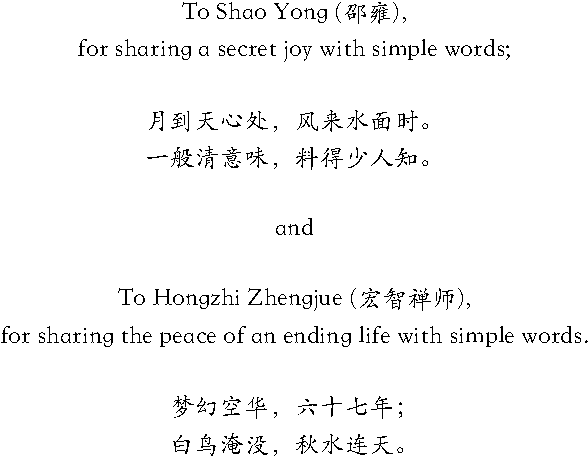
\includegraphics{images/dedication.pdf}
\end{center}

\setlength{\abovedisplayskip}{-5pt}
\setlength{\abovedisplayshortskip}{-5pt}

{
\hypersetup{linkcolor=black}
\setcounter{tocdepth}{2}
\tableofcontents
}
\listoftables
\listoffigures
\chapter*{Prefacio}\label{prefacio}


Este libro fue creado con la intención de ayudar a los estudiantes de
pregrado, especialización, maestría e investigadores a crear gráficos
estadísticos con las herramientas básicas de \proglang{R}. Como
complemento, recomendamos a los lectores el libro
\citet{hernandez_usuga} que muestra cómo usar \proglang{R} para realizar
diversos procedimiento estadísticos.

\section*{Estructura del libro}\label{estructura-del-libro}


En el capítulo \ref{intro} se presenta una introducción breve de
\proglang{R}, sus orígenes, la instalación, tipos de objetos y una guía
de estilo para escribir en \proglang{R}.

\section*{Software information and
conventions}\label{software-information-and-conventions}


Para realizar este libro usamos los paquetes \textbf{knitr}\index{knitr}
\citep{xie2015} y \textbf{bookdown}\index{bookdown} \citep{R-bookdown}
que permiten unir la ventajas de \LaTeX y \proglang{R} en un mismo
archivo.

En todo el libro se presentarán códigos que el lector puede copiar y
pegar en su consola de \proglang{R} para obtener los mismos resultados
aquí presentados. Los códigos se destacan en una caja de color beis (o
beige) similar a la mostrada a continuación.

\begin{Shaded}
\begin{Highlighting}[]
\DecValTok{4} \OperatorTok{+}\StringTok{ }\DecValTok{6}
\NormalTok{a <-}\StringTok{ }\KeywordTok{c}\NormalTok{(}\DecValTok{1}\NormalTok{, }\DecValTok{5}\NormalTok{, }\DecValTok{6}\NormalTok{)}
\DecValTok{5} \OperatorTok{*}\StringTok{ }\NormalTok{a}
\DecValTok{1}\OperatorTok{:}\DecValTok{10}
\end{Highlighting}
\end{Shaded}

Los resultados o salidas obtenidos de cualquier código se destacan con
dos símbolos de númeral (\texttt{\#\#}) al inicio de cada línea o
renglón, esto quiere decir que todo lo que inicie con \texttt{\#\#} son
resultados obtenidos y \textbf{NO} los debe copiar. Abajo se muestran
los resultados obtenidos luego de correr el código anterior.

\begin{verbatim}
## [1] 10
\end{verbatim}

\begin{verbatim}
## [1]  5 25 30
\end{verbatim}

\begin{verbatim}
##  [1]  1  2  3  4  5  6  7  8  9 10
\end{verbatim}

\section*{Bloques informativos}\label{bloques-informativos}


En varias partes del libro usaremos bloques informativos para resaltar
algún aspecto importante. Abajo se encuentra un ejemplo de los bloques y
su significado.

\BeginKnitrBlock{rmdnote}
Este bloque sirve para una nota aclaratoria.
\EndKnitrBlock{rmdnote}

\BeginKnitrBlock{rmdtip}
Este bloque sirve para una sugerencia.
\EndKnitrBlock{rmdtip}

\BeginKnitrBlock{rmdwarning}
Este bloque sirve para una advertencia.
\EndKnitrBlock{rmdwarning}

\section*{Agradecimientos}\label{agradecimientos}


Agradecemos a nuestros estudiantes, profesores y colegas que han leído
el manuscrito y se han tomado el trabajo de escribirnos dándonos sus
sugerencias y comentarios para mejorar continuamente este material.

\BeginKnitrBlock{flushright}
Freddy Hernández Barajas

Juan Carlos Correa Morales
\EndKnitrBlock{flushright}

\chapter*{Sobre los autores}\label{sobre-los-autores}


Freddy Hernández Barajas es profesor asistente de la Universidad
Nacional de Colombia adscrito a la Escuela de Estadística de la Facultad
de Ciencias.

\href{mailto:fhernanb@unal.edu.co}{\nolinkurl{fhernanb@unal.edu.co}}

Juan Carlos Correa Morales es profesor asociado de la Universidad
Nacional de Colombia adscrito a la Escuela de Estadística de la Facultad
de Ciencias.

\href{mailto:jccorreamorales@gmail.com}{\nolinkurl{jccorreamorales@gmail.com}}

\mainmatter

\chapter{\texorpdfstring{Introducción
\label{intro}}{Introducción }}\label{introduccion}

\section{Orígenes} \label{sec:origenes}

\proglang{R} es un lenguaje de programación usado para realizar
procedimientos estadísticos y gráficos de alto nivel, este lenguaje fue
creado en 1993 por los profesores e investigadores Robert Gentleman y
Ross Ihaka. Inicialmente el lenguaje se usó para apoyar los cursos que
tenían a su cargo los profesores, pero luego de ver la utilidad de la
herramienta desarrollada, decidieron colocar copias de \proglang{R} en
StatLib. A partir de 1995 el código fuente de \proglang{R} está
disponible bajo licencia GNU GPL para sistemas operativos Windows,
Macintosh y distribuciones Unix/Linux. La comunidad de usuarios de
\proglang{R} en el mundo es muy grande y los usuarios cuentan con
diferentes espacios para interactuar, a continuación una lista no
exhaustiva de los sitios más populares relacionados con \proglang{R}:

\begin{itemize}
\tightlist
\item
  \href{https://www.r-bloggers.com/}{Rbloggers}.
\item
  \href{http://r-es.org/}{Comunidad hispana de \proglang{R}}.
\item
  \href{http://r.789695.n4.nabble.com/}{Nabble}.
\item
  \href{http://r-br.2285057.n4.nabble.com/}{Foro en portugués}.
\item
  \href{http://stackoverflow.com/questions/tagged/r}{Stackoverflow}.
\item
  \href{http://stats.stackexchange.com/questions/tagged/r}{Cross
  Validated}.
\item
  \href{https://stat.ethz.ch/mailman/listinfo/r-help}{\proglang{R}-Help
  Mailing List}.
\item
  \href{http://blog.revolutionanalytics.com/}{Revolutions}.
\item
  \href{https://www.r-statistics.com/}{\proglang{R}-statistics blog}.
\item
  \href{https://rdatamining.wordpress.com/}{RDataMining}.
\end{itemize}

\begin{figure}

{\centering 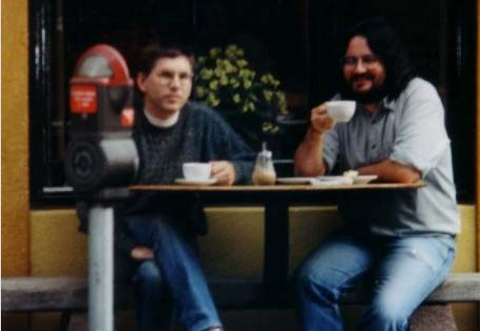
\includegraphics[width=0.5\linewidth]{images/Robert_Roos} 

}

\caption{Robert Gentleman (izquierda) y Ross Ihaka (derecha) creadores de R.}\label{fig:unnamed-chunk-7}
\end{figure}

\section{Descarga e instalación} \label{sec:descarga}

Para realizar la instalación de \proglang{R} usted debe visitar la
página del CRAN (\textit{Comprehensive R Archive Network}) disponible en
este \href{https://cran.r-project.org/}{enlace}. Una vez ingrese a la
página encontrará un cuadro similar al mostrado en la Figura
\ref{fig:cran} donde aparecen los enlaces de la instalación para los
sistemas operativos Linux, Mac y Windows.

\begin{figure}

{\centering 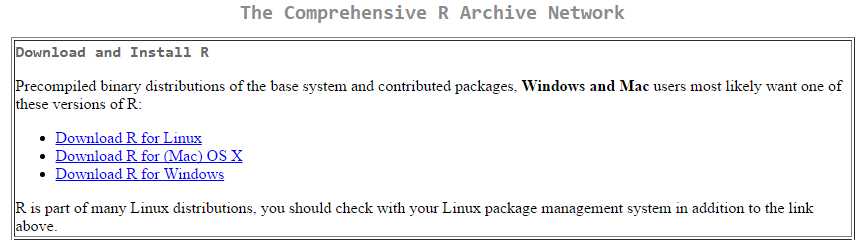
\includegraphics{images/cran} 

}

\caption{Página del Cran.}\label{fig:cran}
\end{figure}

Supongamos que se desea instalar \proglang{R} en Windows, para esto se
debe dar clic sobre el hiperenlace
\textcolor{BurntOrange}{Download R for Windows} de la Figura
\ref{fig:cran}. Una vez hecho esto se abrirá una página con el contenido
mostrado en la Figura \ref{fig:inst1}. Una vez ingrese a esa nueva
página usted debe dar clic sobre el hiperenlace
\textcolor{BurntOrange}{install R for the first time} como es señalado
por la flecha roja en la Figura \ref{fig:inst1}.

\begin{figure}

{\centering 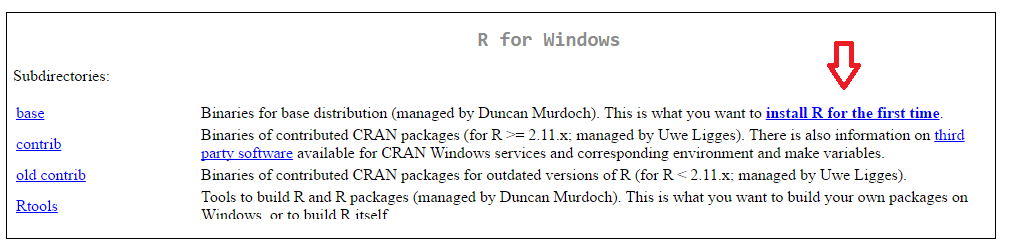
\includegraphics{images/instalacion1} 

}

\caption{Página de instalación para la primera ocasión.}\label{fig:inst1}
\end{figure}

Luego de esto se abrirá otra página con un encabezado similar al
mostrado en la Figura \ref{fig:inst2}, al momento de capturar la figura
la versión actual de \proglang{R} era 3.2.5 pero seguramente en este
momento usted tendrá disponible una versión actualizada. Una vez allí
uste debe dar clic sobre
\textcolor{BurntOrange}{Download R 3.2.5 for Windows} como es señalado
por la flecha verde. Luego de esto se descargará el instalador
\proglang{R} en el computador el cual deberá ser instalado con las
opciones que vienen por defecto.

\begin{figure}

{\centering 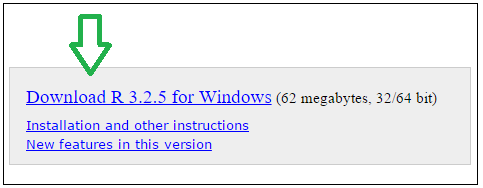
\includegraphics[width=0.5\linewidth]{images/instalacion2} 

}

\caption{Página de descarga.}\label{fig:inst2}
\end{figure}

Se recomienda observar el siguiente video didáctico de instalación de
\proglang{R} disponible en este
\href{http://tinyurl.com/jd7b9ks}{enlace} para facilitar la tarea de
instalación.

\section{Apariencia del programa} \label{sec:apariencia}

Una vez que esté instalado \proglang{R} en su computador, usted podrá
acceder a él por la lista de programas o por medio del acceso directo
que quedó en el escritorio, en la Figura \ref{fig:rlogo} se muestra la
apariencia del acceso directo para ingresar a \proglang{R}.

\begin{figure}

{\centering 
\includegraphics[width=0.33\linewidth]{images/rlogo} 

}

\caption{Apariencia del acceso directo para ingresar a R.}\label{fig:rlogo}
\end{figure}

Al abrir \proglang{R} aparecerá en la pantalla de su computador algo
similar a lo que está en la Figura \ref{fig:pantalla}. La ventana
izquierda se llama consola y es donde se ingresan las instrucciones, una
vez que se construye un gráfico se activa otra ventana llamada ventana
gráfica. Cualquier usuario puede modificar la posición y tamaños de
estas ventanas, puede cambiar el tipo y tamaño de las letras en la
consola, para hacer esto se deben explorar las opciones de
\textit{editar} en la barra de herramientas.

\begin{figure}

{\centering 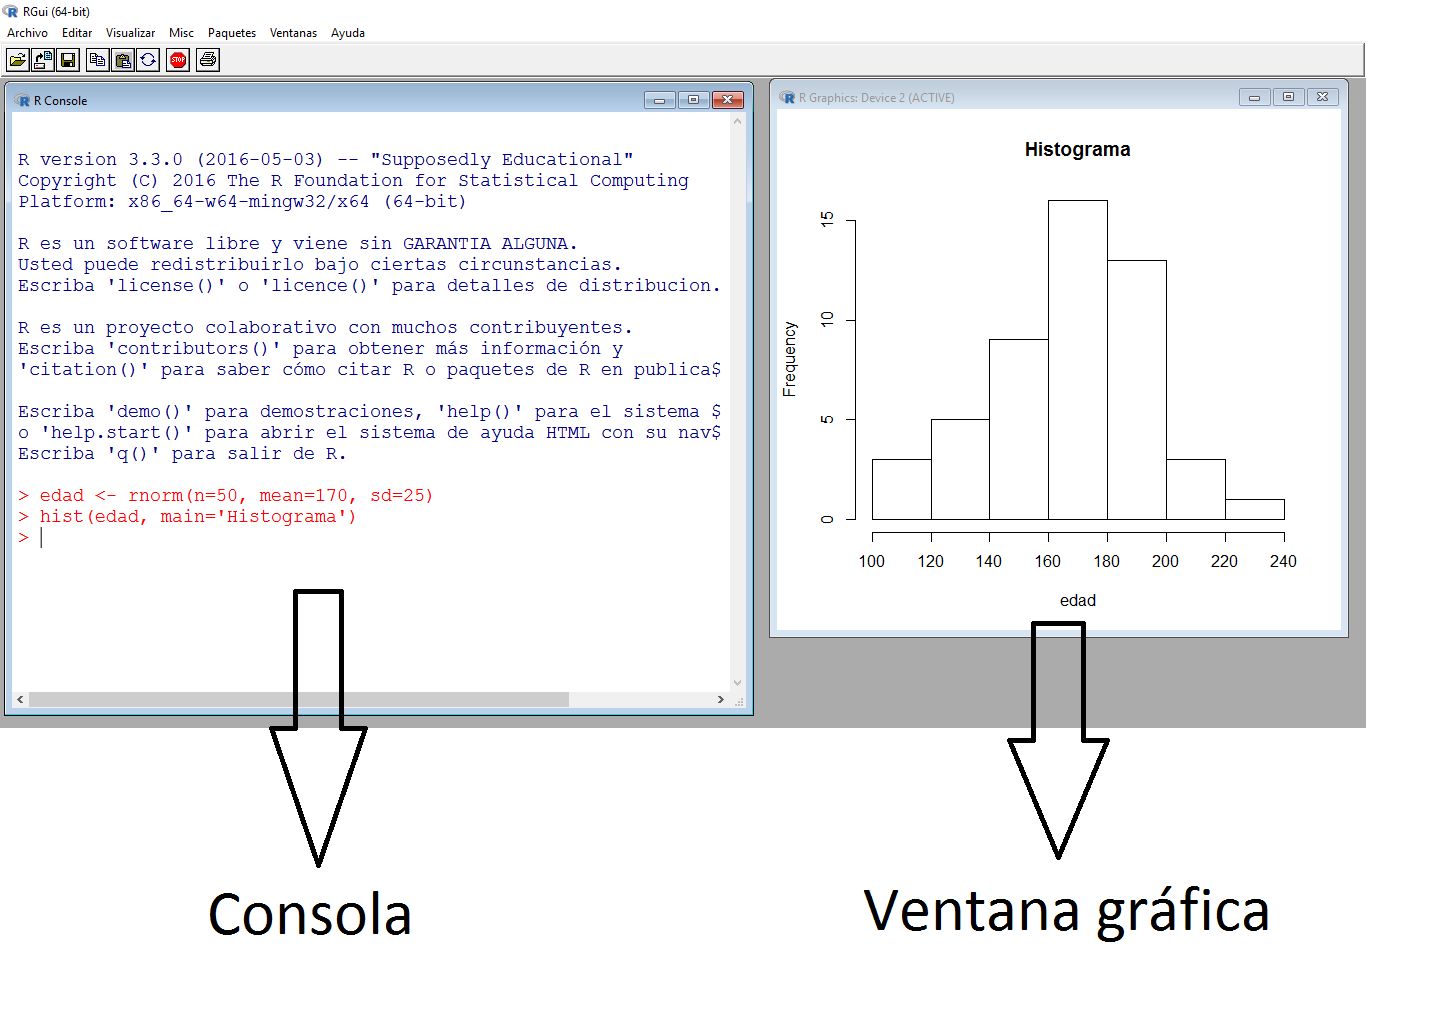
\includegraphics{images/Rpantallazo} 

}

\caption{Apariencia de R.}\label{fig:pantalla}
\end{figure}

\section{Tipos de objetos} \label{sec:objetos}

En \proglang{R} existen varios tipos de objectos \index{objetos} que
permiten que el usuario pueda almacenar la información para realizar
procedimientos estadísticos y gráficos. Los principales objetos en
\proglang{R} son vectores, matrices, arreglos, marcos de datos y listas.
A continuación se presentan las características de estos objetos y la
forma para crearlos.

\subsection{Vectores}

Los vectores \index{vectores} son arreglos ordenados en los cuales se
puede almacenar información de tipo numérico (variable cuantitativa),
alfanumérico (variable cualitativa) o lógico (\texttt{TRUE} o
\texttt{FALSE}), pero no mezclas de éstos. La función de \proglang{R}
para crear un vector es \texttt{c()} y que significa concatenar; dentro
de los paréntesis de esta función se ubica la información a almacenar.
Una vez construído el vector se acostumbra a etiquetarlo con un nombre
corto y representativo de la información que almacena, la asignación se
hace por medio del operador \texttt{\textless{}-} entre el nombre y el
vector.

A continuación se presenta un ejemplo de cómo crear tres vectores que
contienen las respuestas de cinco personas a tres preguntas que se les
realizaron.

\begin{Shaded}
\begin{Highlighting}[]
\NormalTok{edad <-}\StringTok{ }\KeywordTok{c}\NormalTok{(}\DecValTok{15}\NormalTok{, }\DecValTok{19}\NormalTok{, }\DecValTok{13}\NormalTok{, }\OtherTok{NA}\NormalTok{, }\DecValTok{20}\NormalTok{)}
\NormalTok{deporte <-}\StringTok{ }\KeywordTok{c}\NormalTok{(}\OtherTok{TRUE}\NormalTok{, }\OtherTok{TRUE}\NormalTok{, }\OtherTok{NA}\NormalTok{, }\OtherTok{FALSE}\NormalTok{, }\OtherTok{TRUE}\NormalTok{)}
\NormalTok{comic.fav <-}\StringTok{ }\KeywordTok{c}\NormalTok{(}\OtherTok{NA}\NormalTok{, }\StringTok{'Superman'}\NormalTok{, }\StringTok{'Batman'}\NormalTok{, }\OtherTok{NA}\NormalTok{, }\StringTok{'Batman'}\NormalTok{)}
\end{Highlighting}
\end{Shaded}

El vector \texttt{edad} es un vector cuantitativo y contiene las edades
de las 5 personas. En la cuarta posición del vector se colocó el símbolo
\texttt{NA} que significa \textit{Not Available} debido a que no se
registró la edad para esa persona. Al hacer una asignación se acostumbra
a dejar un espacio antes y después del operador \texttt{\textless{}-} de
asignación. El segundo vector es llamado \texttt{deporte} y es un vector
lógico que almacena las respuestas a la pregunta de si la persona
practica deporte, nuevamente aquí hay un \texttt{NA} para la tercera
persona. El último vector \texttt{comic.fav} contiene la información del
cómic favorito de cada persona, como esta variable es cualitativa es
necesario usar las comillas
\texttt{\textquotesingle{}\ \textquotesingle{}} para encerrar las
respuestas.

\BeginKnitrBlock{rmdwarning}
Cuando se usa \texttt{NA} para representar una información
\textit{Not Available} no se deben usar comillas.
\EndKnitrBlock{rmdwarning}

\BeginKnitrBlock{rmdnote}
Es posible usar comillas sencillas
\texttt{\textquotesingle{}foo\textquotesingle{}} o comillas dobles
\texttt{"foo"} para ingresar valores de una variable cualitativa.
\EndKnitrBlock{rmdnote}

Si se desea ver lo que está almacenado en cada uno de estos vectores, se
debe escribir en la consola de \proglang{R} el nombre de uno de los
objetos y luego se presiona la tecla \textit{enter} o \textit{intro}, al
realizar esto lo que se obtiene se muestra a continuación.

\begin{Shaded}
\begin{Highlighting}[]
\NormalTok{edad}
\end{Highlighting}
\end{Shaded}

\begin{verbatim}
## [1] 15 19 13 NA 20
\end{verbatim}

\begin{Shaded}
\begin{Highlighting}[]
\NormalTok{deporte}
\end{Highlighting}
\end{Shaded}

\begin{verbatim}
## [1]  TRUE  TRUE    NA FALSE  TRUE
\end{verbatim}

\begin{Shaded}
\begin{Highlighting}[]
\NormalTok{comic.fav}
\end{Highlighting}
\end{Shaded}

\begin{verbatim}
## [1] NA         "Superman" "Batman"   NA        
## [5] "Batman"
\end{verbatim}

\subsection{Matrices}

Las matrices \index{matrices} son arreglos rectangulares de filas y
columnas con información numérica, alfanumérica o lógica. Para construir
una matriz se usa la función \texttt{matrix(\ )}. Por ejemplo, para
crear una matriz de 4 filas y 5 columnas (de dimensión \(4 \times 5\))
con los primeros 20 números positivos se escribe el código siguiente en
la consola.

\begin{Shaded}
\begin{Highlighting}[]
\NormalTok{mimatriz <-}\StringTok{ }\KeywordTok{matrix}\NormalTok{(}\DataTypeTok{data=}\DecValTok{1}\OperatorTok{:}\DecValTok{20}\NormalTok{, }\DataTypeTok{nrow=}\DecValTok{4}\NormalTok{, }\DataTypeTok{ncol=}\DecValTok{5}\NormalTok{, }\DataTypeTok{byrow=}\OtherTok{FALSE}\NormalTok{)}
\end{Highlighting}
\end{Shaded}

El argumento \texttt{data} de la función sirve para indicar los datos
que se van a almacenar en la matriz, los argumentos \texttt{nrow} y
\texttt{ncol} sirven para definir la dimensión de la matriz y por último
el argumento \texttt{byrow} sirve para indicar si la información
contenida en \texttt{data} se debe ingresar por filas o no. Para
observar lo que quedó almacenado en el objeto \texttt{mimatriz} se
escribe en la consola el nombre del objeto seguido de la tecla
\textit{enter} o \textit{intro}.

\begin{Shaded}
\begin{Highlighting}[]
\NormalTok{mimatriz}
\end{Highlighting}
\end{Shaded}

\begin{verbatim}
##      [,1] [,2] [,3] [,4] [,5]
## [1,]    1    5    9   13   17
## [2,]    2    6   10   14   18
## [3,]    3    7   11   15   19
## [4,]    4    8   12   16   20
\end{verbatim}

\subsection{Arreglos}

Un arreglo \index{arreglo} es una matriz de varias dimensiones con
información numérica, alfanumérica o lógica. Para construir una arreglo
se usa la función \texttt{array(\ )}. Por ejemplo, para crear un arreglo
de \(3 \times 4 \times 2\) con las primeras 24 letras minúsculas del
alfabeto se escribe el siguiente código.

\begin{Shaded}
\begin{Highlighting}[]
\NormalTok{miarray <-}\StringTok{ }\KeywordTok{array}\NormalTok{(}\DataTypeTok{data=}\NormalTok{letters[}\DecValTok{1}\OperatorTok{:}\DecValTok{24}\NormalTok{], }\DataTypeTok{dim=}\KeywordTok{c}\NormalTok{(}\DecValTok{3}\NormalTok{, }\DecValTok{4}\NormalTok{, }\DecValTok{2}\NormalTok{))}
\end{Highlighting}
\end{Shaded}

El argumento \texttt{data} de la función sirve para indicar los datos
que se van a almacenar en el arreglo y el argumento \texttt{dim} sirve
para indicar las dimensiones del arreglo. Para observar lo que quedó
almacenado en el objeto \texttt{miarray} se escribe en la consola lo
siguiente.

\begin{Shaded}
\begin{Highlighting}[]
\NormalTok{miarray}
\end{Highlighting}
\end{Shaded}

\begin{verbatim}
## , , 1
## 
##      [,1] [,2] [,3] [,4]
## [1,] "a"  "d"  "g"  "j" 
## [2,] "b"  "e"  "h"  "k" 
## [3,] "c"  "f"  "i"  "l" 
## 
## , , 2
## 
##      [,1] [,2] [,3] [,4]
## [1,] "m"  "p"  "s"  "v" 
## [2,] "n"  "q"  "t"  "w" 
## [3,] "o"  "r"  "u"  "x"
\end{verbatim}

\subsection{Marco de datos}

El marco de datos \index{marco de datos} o \textit{data frame} es uno de
los objetos más utilizados porque permite agrupar vectores con
información de diferente tipo (numérica, alfanumérica o lógica) en un
mismo objeto, la única restricción es que los vectores deben tener la
misma longitud. Para crear un marco de datos se usa la función
\texttt{data.frame(\ )}, como ejemplo vamos a crear un marco de datos
con los vectores \texttt{edad}, \texttt{deporte} y \texttt{comic.fav}
definidos anteriormente.

\begin{Shaded}
\begin{Highlighting}[]
\NormalTok{mimarco <-}\StringTok{ }\KeywordTok{data.frame}\NormalTok{(edad, deporte, comic.fav)}
\end{Highlighting}
\end{Shaded}

Una vez creado el objeto \texttt{mimarco} podemos ver el objeto
escribiendo su nombre en la consola, a continuación se muestra lo que se
obtiene.

\begin{Shaded}
\begin{Highlighting}[]
\NormalTok{mimarco}
\end{Highlighting}
\end{Shaded}

\begin{verbatim}
##   edad deporte comic.fav
## 1   15    TRUE      <NA>
## 2   19    TRUE  Superman
## 3   13      NA    Batman
## 4   NA   FALSE      <NA>
## 5   20    TRUE    Batman
\end{verbatim}

De la salida anterior vemos que el marco de datos tiene 3 variables
(columnas) cuyos nombres coinciden con los nombres de los vectores
creados anteriormente, los números consecutivos al lado izquierdo son
sólo de referencia y permiten identificar la información para cada
persona en la base de datos.

\subsection{Listas}

Las listas \index{lista} son otro tipo de objeto muy usado para
almacenar objetos de diferente tipo. La instrucción para crear una lista
es \texttt{list(\ )}. A continuación vamos a crear una lista que
contiene tres objetos: un vector con 5 números aleatorios llamado
\texttt{mivector}, una matriz de dimensión \(6 \times 2\) con los
primeros doce números enteros positivos llamada \texttt{matriz2} y el
tercer objeto será el marco de datos \texttt{mimarco} creado en el
apartado anterior. Las instrucciones para crear la lista requerida se
muestran a continuación.

\begin{Shaded}
\begin{Highlighting}[]
\KeywordTok{set.seed}\NormalTok{(}\DecValTok{12345}\NormalTok{)}
\NormalTok{mivector <-}\StringTok{ }\KeywordTok{runif}\NormalTok{(}\DataTypeTok{n=}\DecValTok{5}\NormalTok{)}
\NormalTok{matriz2 <-}\StringTok{ }\KeywordTok{matrix}\NormalTok{(}\DataTypeTok{data=}\DecValTok{1}\OperatorTok{:}\DecValTok{12}\NormalTok{, }\DataTypeTok{ncol=}\DecValTok{6}\NormalTok{)}
\NormalTok{milista <-}\StringTok{ }\KeywordTok{list}\NormalTok{(}\DataTypeTok{E1=}\NormalTok{mivector, }\DataTypeTok{E2=}\NormalTok{matriz2, }\DataTypeTok{E3=}\NormalTok{mimarco)}
\end{Highlighting}
\end{Shaded}

La función \texttt{set.seed} de la línea número 1 sirve para fijar la
semilla de tal manera que los números aleatorios generados en la segunda
línea con la función \texttt{runif} sean siempre los mismos. En la
última línea del código anterior se construye la lista, dentro de la
función \texttt{list} se colocan los tres objetos \texttt{mivector},
\texttt{matriz2} y \texttt{mimarco}. Es posible colocarle un nombre
especial a cada uno de los elementos de la lista, en este ejemplo se
colocaron los nombres \texttt{E1}, \texttt{E2} y \texttt{E3} para cada
uno de los tres elementos. Para observar lo que quedó almacenado en la
lista se escribe \texttt{milista} en la consola y el resultado se
muestra a continuación.

\begin{Shaded}
\begin{Highlighting}[]
\NormalTok{milista}
\end{Highlighting}
\end{Shaded}

\begin{verbatim}
## $E1
## [1] 0.7209 0.8758 0.7610 0.8861 0.4565
## 
## $E2
##      [,1] [,2] [,3] [,4] [,5] [,6]
## [1,]    1    3    5    7    9   11
## [2,]    2    4    6    8   10   12
## 
## $E3
##   edad deporte comic.fav
## 1   15    TRUE      <NA>
## 2   19    TRUE  Superman
## 3   13      NA    Batman
## 4   NA   FALSE      <NA>
## 5   20    TRUE    Batman
\end{verbatim}

\section{Guía de estilo para la escritura en R} \label{sec:estilo}

Así como en el español existen reglas ortográficas, la escritura de
códigos en \proglang{R} también tiene unas reglas que se recomienda
seguir para evitar confusiones. Tener una buena guía de estilo
\index{guía de estilo} es importante para que el código creado por usted
sea fácilmente entendido por sus lectores \citet{rpackages}. No existe
una única y mejor guía de estilo para escritura en \proglang{R}, sin
embargo aquí vamos a mostrar unas sugerencias basadas en la guía llamada
\href{https://google.github.io/styleguide/Rguide.xml}{\textit{Google's R style guide}}.

\subsection{Nombres de los archivos}

Se sugiere que el nombre usado para nombrar un archivo tenga sentido y
que termine con extensión .R. A continuación dos ejemplos de como
nombrar mal y bien un archivo.

\begin{itemize}
    \item Mal: \verb|hola.R|
    \item Bien: \verb|analisis_icfes.R|
\end{itemize}

\subsection{Nombres de los objetos}

Se recomienda no usar los símbolos \texttt{\_} y \texttt{-} dentro de
los nombres de objetos. Para las variables es preferible usar letras
minúsculas y separar las palabras con puntos (\texttt{peso.maiz}) o
utilizar la notación camello iniciando en minúscula (\texttt{pesoMaiz}).
Para las funciones se recomienda usar la notación camello iniciando
todas la palabras en mayúscula (\texttt{PlotRes}). Para los nombres de
las constantes se recomienda que inicien con la letra k
(\texttt{kPrecioBus}). A continuación ejemplos de buenas y malas
prácticas.

Para variables:

\begin{itemize}
    \item Bien: \verb|avg.clicks|
    \item Aceptable: \verb|avgClicks|
    \item Mal: \verb|avg_Clicks|
\end{itemize}

Para funciones:

\begin{itemize}
    \item Bien: \verb|CalculateAvgClicks| 
    \item Mal: \verb|calculate_avg_clicks| , \verb|calculateAvgClicks|
\end{itemize}

\subsection{Longitud de una línea de código}

Se recomienda que cada línea tenga como máximo 80 caracteres. Si una
línea es muy larga se debe cortar siempre por una coma.

\subsection{Espacios}

Use espacios alrededor de todos los operadores binarios (=, +, -,
\textless{}-, etc.). Los espacios alrededor del símbolo ``='' son
opcionales cuando se usan para ingresar valores dentro de una función.
Así como en español, nunca coloque espacio antes de una coma, pero
siempre use espacio luego de una coma. A continuación ejemplos de buenas
y malas prácticas.

\begin{Shaded}
\begin{Highlighting}[]
\NormalTok{tab <-}\StringTok{ }\KeywordTok{table}\NormalTok{(df[df}\OperatorTok{$}\NormalTok{days }\OperatorTok{<}\StringTok{ }\DecValTok{0}\NormalTok{, }\DecValTok{2}\NormalTok{])  }\CommentTok{# Bien}
\NormalTok{tot <-}\StringTok{ }\KeywordTok{sum}\NormalTok{(x[, }\DecValTok{1}\NormalTok{])                }\CommentTok{# Bien}
\NormalTok{tot <-}\StringTok{ }\KeywordTok{sum}\NormalTok{(x[}\DecValTok{1}\NormalTok{, ])                }\CommentTok{# Bien}
\NormalTok{tab <-}\StringTok{ }\KeywordTok{table}\NormalTok{(df[df}\OperatorTok{$}\NormalTok{days}\OperatorTok{<}\DecValTok{0}\NormalTok{, }\DecValTok{2}\NormalTok{])    }\CommentTok{# Faltan espacios alrededor '<' }
\NormalTok{tab <-}\StringTok{ }\KeywordTok{table}\NormalTok{(df[df}\OperatorTok{$}\NormalTok{days }\OperatorTok{<}\StringTok{ }\DecValTok{0}\NormalTok{,}\DecValTok{2}\NormalTok{])   }\CommentTok{# Falta espacio luego de coma}
\NormalTok{tab <-}\StringTok{ }\KeywordTok{table}\NormalTok{(df[df}\OperatorTok{$}\NormalTok{days }\OperatorTok{<}\StringTok{ }\DecValTok{0}\NormalTok{ , }\DecValTok{2}\NormalTok{]) }\CommentTok{# Sobra espacio antes de coma}
\NormalTok{tab<-}\StringTok{ }\KeywordTok{table}\NormalTok{(df[df}\OperatorTok{$}\NormalTok{days }\OperatorTok{<}\StringTok{ }\DecValTok{0}\NormalTok{, }\DecValTok{2}\NormalTok{])   }\CommentTok{# Falta espacio antes de '<-'}
\NormalTok{tab<-}\KeywordTok{table}\NormalTok{(df[df}\OperatorTok{$}\NormalTok{days }\OperatorTok{<}\StringTok{ }\DecValTok{0}\NormalTok{, }\DecValTok{2}\NormalTok{])    }\CommentTok{# Falta espacio alrededor de '<-'}
\NormalTok{tot <-}\StringTok{ }\KeywordTok{sum}\NormalTok{(x[,}\DecValTok{1}\NormalTok{])                 }\CommentTok{# Falta espacio luego de coma}
\NormalTok{tot <-}\StringTok{ }\KeywordTok{sum}\NormalTok{(x[}\DecValTok{1}\NormalTok{,])                 }\CommentTok{# Falta espacio luego de coma}
\end{Highlighting}
\end{Shaded}

Otra buena práctica es colocar espacio antes de un paréntesis excepto
cuando se llama una función.

\begin{Shaded}
\begin{Highlighting}[]
\ControlFlowTok{if}\NormalTok{ (debug)    }\CommentTok{# Correcto}
\ControlFlowTok{if}\NormalTok{(debug)     }\CommentTok{# Funciona pero no se recomienda}
\KeywordTok{colMeans}\NormalTok{ (x)  }\CommentTok{# Funciona pero no se recomienda}
\end{Highlighting}
\end{Shaded}

Espacios extras pueden ser usados si con esto se mejora la apariencia
del código, ver el ejemplo siguiente.

\begin{Shaded}
\begin{Highlighting}[]
\KeywordTok{plot}\NormalTok{(}\DataTypeTok{x    =}\NormalTok{ x.coord,}
     \DataTypeTok{y    =}\NormalTok{ data.mat[, }\KeywordTok{MakeColName}\NormalTok{(metric, ptiles[}\DecValTok{1}\NormalTok{], }\StringTok{"roiOpt"}\NormalTok{)],}
     \DataTypeTok{ylim =}\NormalTok{ ylim,}
     \DataTypeTok{xlab =} \StringTok{"dates"}\NormalTok{,}
     \DataTypeTok{ylab =}\NormalTok{ metric,}
     \DataTypeTok{main =}\NormalTok{ (}\KeywordTok{paste}\NormalTok{(metric, }\StringTok{" for 3 samples "}\NormalTok{, }\DataTypeTok{sep =} \StringTok{""}\NormalTok{)))}
\end{Highlighting}
\end{Shaded}

No coloque espacios alrededor del código que esté dentro de paréntesis
\texttt{(\ )} o corchetes \texttt{{[}\ {]}}, la única excepción es luego
de una coma, ver el ejemplo siguiente.

\begin{Shaded}
\begin{Highlighting}[]
\ControlFlowTok{if}\NormalTok{ (condicion)    }\CommentTok{# Correcto }
\NormalTok{x[}\DecValTok{1}\NormalTok{, ]            }\CommentTok{# Correcto}
\ControlFlowTok{if}\NormalTok{ ( condicion )  }\CommentTok{# Sobran espacios alrededor de condicion}
\NormalTok{x[}\DecValTok{1}\NormalTok{,]             }\CommentTok{# Se necesita espacio luego de coma}
\end{Highlighting}
\end{Shaded}

Los signos de agrupación llaves \texttt{\{\ \}} se utilizan para agrupar
bloques de código y se recomienda que nunca una llave abierta
\texttt{\{} esté sola en una línea; una llave cerrada \texttt{\}} si
debe ir sola en su propia línea. Se pueden omitir las llaves cuando el
bloque de instrucciones esté formado por una sola línea pero esa línea
de código NO debe ir en la misma línea de la condición. A continuación
dos ejemplos de lo que se recomienda.

\begin{Shaded}
\begin{Highlighting}[]
\ControlFlowTok{if}\NormalTok{ (}\KeywordTok{is.null}\NormalTok{(ylim)) \{                     }\CommentTok{# Correcto}
\NormalTok{  ylim <-}\StringTok{ }\KeywordTok{c}\NormalTok{(}\DecValTok{0}\NormalTok{, }\FloatTok{0.06}\NormalTok{)}
\NormalTok{\}}

\ControlFlowTok{if}\NormalTok{ (}\KeywordTok{is.null}\NormalTok{(ylim))                       }\CommentTok{# Correcto}
\NormalTok{  ylim <-}\StringTok{ }\KeywordTok{c}\NormalTok{(}\DecValTok{0}\NormalTok{, }\FloatTok{0.06}\NormalTok{)}

\ControlFlowTok{if}\NormalTok{ (}\KeywordTok{is.null}\NormalTok{(ylim)) ylim <-}\StringTok{ }\KeywordTok{c}\NormalTok{(}\DecValTok{0}\NormalTok{, }\FloatTok{0.06}\NormalTok{)    }\CommentTok{# Aceptable}

\ControlFlowTok{if}\NormalTok{ (}\KeywordTok{is.null}\NormalTok{(ylim))                       }\CommentTok{# No se recomienda}
\NormalTok{\{        }
\NormalTok{  ylim <-}\StringTok{ }\KeywordTok{c}\NormalTok{(}\DecValTok{0}\NormalTok{, }\FloatTok{0.06}\NormalTok{)}
\NormalTok{\}}
    
\ControlFlowTok{if}\NormalTok{ (}\KeywordTok{is.null}\NormalTok{(ylim)) \{ylim <-}\StringTok{ }\KeywordTok{c}\NormalTok{(}\DecValTok{0}\NormalTok{, }\FloatTok{0.06}\NormalTok{)\}}
\CommentTok{# Frente a la llave \{ no debe ir nada}
\CommentTok{# la llave de cierre \} debe ir sola}
\end{Highlighting}
\end{Shaded}

La sentencia else debe ir siempre entre llaves \texttt{\}\ \{}, ver el
siguiente ejemplo.

\begin{Shaded}
\begin{Highlighting}[]
\ControlFlowTok{if}\NormalTok{ (condition) \{         }
\NormalTok{  one or more lines}
\NormalTok{\} }\ControlFlowTok{else}\NormalTok{ \{                 }\CommentTok{# Correcto}
\NormalTok{  one or more lines}
\NormalTok{\}}


\ControlFlowTok{if}\NormalTok{ (condition) \{         }
\NormalTok{  one or more lines}
\NormalTok{\}}
\ControlFlowTok{else}\NormalTok{ \{                   }\CommentTok{# Incorrecto}
\NormalTok{  one or more lines}
\NormalTok{\}}


\ControlFlowTok{if}\NormalTok{ (condition)           }
\NormalTok{  one line}
\ControlFlowTok{else}                     \CommentTok{# Incorrecto}
\NormalTok{  one line}
\end{Highlighting}
\end{Shaded}

\subsection{Asignación}

Para realizar asignaciones se recomienda usar el símbolo
\texttt{\textless{}-}, el símbolo de igualdad \texttt{=} no se
recomienda usarlo para asignaciones.

\begin{Shaded}
\begin{Highlighting}[]
\NormalTok{x <-}\StringTok{ }\DecValTok{5}  \CommentTok{# Correcto}
\NormalTok{x =}\StringTok{ }\DecValTok{5}   \CommentTok{# No recomendado}
\end{Highlighting}
\end{Shaded}

Para una explicación más detallada sobre el símbolo de asignación se
recomienda visitar este
\href{http://www.win-vector.com/blog/2016/12/the-case-for-using-in-r/}{enlace}.

\subsection{Punto y coma}

No se recomienda colocar varias instrucciones separadas por \texttt{;}
en la misma línea, aunque funciona dificulta la revisión del código.

\begin{Shaded}
\begin{Highlighting}[]
\NormalTok{n <-}\StringTok{ }\DecValTok{100}\NormalTok{; y <-}\StringTok{ }\KeywordTok{rnorm}\NormalTok{(n, }\DataTypeTok{mean=}\DecValTok{5}\NormalTok{); }\KeywordTok{hist}\NormalTok{(y)  }\CommentTok{# No se recomienda}

\NormalTok{n <-}\StringTok{ }\DecValTok{100}                                  \CommentTok{# Correcto}
\NormalTok{y <-}\StringTok{ }\KeywordTok{rnorm}\NormalTok{(n, }\DataTypeTok{mean=}\DecValTok{5}\NormalTok{)}
\KeywordTok{hist}\NormalTok{(y)}
\end{Highlighting}
\end{Shaded}

A pesar de la anterior advertencia es posible que en este libro usemos
el \texttt{;} en algunas ocasiones, si lo hacemos es para ahorrar
espacio en la presentación del código.

\chapter{Gráficos para una variable
cuantitativa}\label{graficos-para-una-variable-cuantitativa}

En este capítulo se presentan funciones para la creación de gráficos con
una sola variable cuantitativa.

\section{\texorpdfstring{Función \texttt{stem} \index{stem}
\index{tallo y hoja}}{Función stem  }}\label{funcion-stem}

Esta función permite crear el gráfico llamado de tallo y hoja. Este
gráfico fue propuesto por Tukey (1977) y a pesar de no ser un gráfico
para presentación definitiva, se utiliza a la vez que el analista recoge
la información para ver rápidamente la distribución de los datos.

¿Qué muestra este gráfico?

\begin{enumerate}
\def\labelenumi{\arabic{enumi}.}
\tightlist
\item
  El centro de la distribución.
\item
  La forma general de la distribución:

  \begin{itemize}
  \tightlist
  \item
    Simétrica: Si las porciones a cada lado del centro son imágenes
    espejos de las otras.
  \item
    Sesgada a la izquierda: Si la cola izquierda (los valores menores)
    es mucho más larga que los de la derecha (los valores mayores).
  \item
    Sesgada a la derecha: Opuesto a la sesgada a la izquierda.
  \end{itemize}
\item
  Desviaciones marcadas de la forma global de la distribución.

  \begin{itemize}
  \tightlist
  \item
    Outliers: Observaciones individuales que caen muy por fuera del
    patrón general de los datos.
  \item
    Gaps: Huecos en la distribución
  \end{itemize}
\end{enumerate}

Ventajas del gráfico:

\begin{enumerate}
\def\labelenumi{\arabic{enumi}.}
\tightlist
\item
  Muy fácil de realizar y puede hacerse a mano.
\item
  Fácil de entender.
\end{enumerate}

Desventajas del gráfico:

\begin{enumerate}
\def\labelenumi{\arabic{enumi}.}
\tightlist
\item
  El gráfico es tosco y no sirve para presentaciones definitivas.
\item
  Funciona cuando el número de observaciones no es muy grande.
\item
  No permite comparar claramente diferentes poblaciones
\end{enumerate}

\subsection*{Ejemplo}\label{ejemplo}


Como ilustración vamos a crear el gráfico de tallo y hoja para la
variable altura (cm) de un grupo de estudiantes de la universidad.
Primero se leerán los datos disponibles en github y luego se usará la
función \texttt{stem} para obtener el gráfico. A continuación el código
usado.

\begin{Shaded}
\begin{Highlighting}[]
\NormalTok{url <-}\StringTok{ 'https://tinyurl.com/k55nnlu'}
\NormalTok{datos <-}\StringTok{ }\KeywordTok{read.table}\NormalTok{(}\DataTypeTok{file=}\NormalTok{url, }\DataTypeTok{header=}\NormalTok{T)}
\KeywordTok{stem}\NormalTok{(datos}\OperatorTok{$}\NormalTok{altura)}
\end{Highlighting}
\end{Shaded}

\begin{verbatim}
## 
##   The decimal point is 1 digit(s) to the right of the |
## 
##   14 | 7
##   15 | 3
##   15 | 679
##   16 | 0001
##   16 | 68888
##   17 | 001334
##   17 | 5678899
##   18 | 000033
##   18 | 88
##   19 | 1
\end{verbatim}

De este gráfico sencillo se puede ver que la variable presenta una mayor
frecuencia para alturas ente 170 y 179 cm y que no tiene una
distribución simétrica.

\section{\texorpdfstring{Función \texttt{boxplot}
\index{boxplot}}{Función boxplot }}\label{funcion-boxplot}

La función \texttt{boxplot} sirve para crear un diagrama de cajas y
bigote para una variable cuantitativa. La estructura de la función
\texttt{boxplot} con los argumentos más comunes de uso se muestran a
continuación.

\begin{Shaded}
\begin{Highlighting}[]
\KeywordTok{boxplot}\NormalTok{(x, formula, data, subset, na.action,}
\NormalTok{        range, width, varwidth, notch, names, }
\NormalTok{        plot, col, log, horizontal, add, ...)}
\end{Highlighting}
\end{Shaded}

Los argumentos de la función \texttt{boxplot} son:

\begin{itemize}
\tightlist
\item
  \texttt{x}: vector numérico con los datos para crear el boxplot.
\item
  \texttt{formula}: fórmula con la estructura
  \texttt{x\ \textasciitilde{}\ g} para indicar que las observaciones en
  el vector \texttt{x} van a ser agrupadas de acuerdo a los niveles del
  factor \texttt{g}.
\item
  \texttt{data}: marco de datos con las variables.
\item
  \texttt{subset}: un vector opcional para especificar un subconjunto de
  observaciones a ser usadas en el proceso de ajuste.
\item
  \texttt{na.action}: una función la cual indica lo que debería pasar
  cuando los datos contienen ``NA's''.
\item
  \texttt{range}: valor numérico que indica la extensión de los bigotes.
  Si es positivo, los bigotes se extenderán hasta el punto más extremo
  de tal manera que el bigote no supere \code{range} veces el rango
  intercuatílico (\(IQ\)). Un valor de cero hace que los bigotes se
  extiendan hasta los datos extremos.
\item
  \texttt{width}: un vector con los anchos relativos de las cajas.
\item
  \texttt{varwidth}: Si es \texttt{TRUE}, las cajas son dibujadas con
  anchos proporcionales a las raíces cuadradas del número de
  observaciones en los grupos.
\item
  \texttt{notch}: si es \texttt{TRUE}, una cuña es dibujada a cada lado
  de las cajas. Cuando las cuñas de dos gráficos de caja no se
  traslapan, entonces las medianas son significativamente diferentes a
  un nivel del 5\%.
\item
  \texttt{names}: un con las etiquetas a ser impresas debajo de cada
  boxplot.
\item
  \texttt{plot}: si es \texttt{TRUE} (por defecto) entonces se produce
  el gráfico, de lo contrario, se producen los resúmenes de los
  boxplots.
\item
  \texttt{col}: vector con los colores a usar en el cuerpo de las cajas.
\item
  \texttt{log}: para indicar si las coordenadas \texttt{x} o \texttt{y}
  o serán graficadas en escala logarítmica.
\item
  \texttt{...}: otros parámetros gráficos que pueden ser pasados como
  argumentos para el boxplot.
\end{itemize}

\subsection*{Ejemplo}\label{ejemplo-1}


Como ilustración vamos a crear dos boxplot para la variable altura (cm)
de un grupo de estudiantes de la universidad, el primer boxplot será
vertical y el segundo horizontal. Primero se leerán los datos
disponibles en github y luego se usará la función \texttt{boxplot} para
obtener ambos gráfico. A continuación el código usado.

\begin{Shaded}
\begin{Highlighting}[]
\NormalTok{url <-}\StringTok{ 'https://tinyurl.com/k55nnlu'}
\NormalTok{datos <-}\StringTok{ }\KeywordTok{read.table}\NormalTok{(}\DataTypeTok{file=}\NormalTok{url, }\DataTypeTok{header=}\NormalTok{T)}

\KeywordTok{par}\NormalTok{(}\DataTypeTok{mfrow=}\KeywordTok{c}\NormalTok{(}\DecValTok{1}\NormalTok{, }\DecValTok{2}\NormalTok{))}
\KeywordTok{boxplot}\NormalTok{(}\DataTypeTok{x=}\NormalTok{datos}\OperatorTok{$}\NormalTok{altura, }\DataTypeTok{ylab=}\StringTok{'Altura (cm)'}\NormalTok{)}
\KeywordTok{boxplot}\NormalTok{(}\DataTypeTok{x=}\NormalTok{datos}\OperatorTok{$}\NormalTok{altura, }\DataTypeTok{xlab=}\StringTok{'Altura (cm)'}\NormalTok{, }\DataTypeTok{horizontal=}\OtherTok{TRUE}\NormalTok{)}
\end{Highlighting}
\end{Shaded}

\begin{figure}
\centering
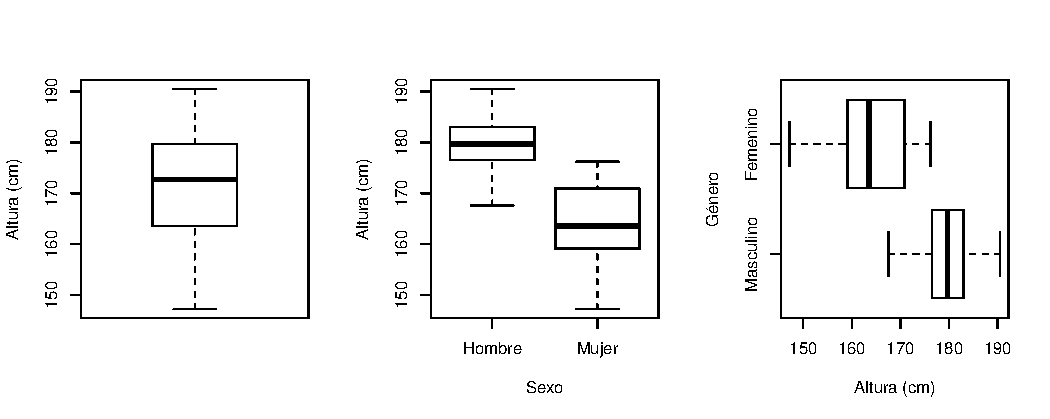
\includegraphics{Graficos_con_R_files/figure-latex/boxplots-1.pdf}
\caption{\label{fig:boxplots}Boxplot para la variable altura.}
\end{figure}

En la Figura \ref{fig:boxplots} se presentan los boxplots obtenidos con
las instrucciones anteriores. El segundo y tercer boxplot son el mismo,
lo único que se modificó fueron los nombres o etiquetas a colocar debajo
de cada boxplot por medio del argumento \texttt{names} y la orientación.

\subsection*{Ejemplo}\label{ejemplo-2}


\index{boxplot comparativo} Es posible crear boxplots comparativos
usando 1 o 2 variables cualitativas. A continuación se construyen dos
boxplots para la variable precio de apartamentos usados en Medellín. En
el primer boxtplot diferencia por la variable balcón (no, si) y en el
segundo se diferencia por los cruces de las variables parqueadero y
ubicación (en Laureles y Poblado).

A continuación se muestra el código necesario para construir los
boxplots. En el primero se usa la fórmula
\texttt{precio\ \textasciitilde{}\ balcon} para crear el boxplot del
precio diferenciando por los dos niveles de la variable balcón. En el
segundo se usa la fórmula
\texttt{precio\ \textasciitilde{}\ ubicacion\ *\ parqueadero} pero se
limitan las ubicaciones a sólo dos, Laureles y Aburrá sur, por esa razón
se usa el parámetro \texttt{subset} para incluir la restricción. Se
agregó también \texttt{drop=TRUE} para que en el segundo boxplot no
aparezcan las otras ubicaciones.

\begin{Shaded}
\begin{Highlighting}[]
\NormalTok{url <-}\StringTok{ 'https://tinyurl.com/hwhb769'}
\NormalTok{datos <-}\StringTok{ }\KeywordTok{read.table}\NormalTok{(url, }\DataTypeTok{header=}\NormalTok{T)}

\KeywordTok{par}\NormalTok{(}\DataTypeTok{mfrow=}\KeywordTok{c}\NormalTok{(}\DecValTok{1}\NormalTok{, }\DecValTok{2}\NormalTok{))}
\KeywordTok{boxplot}\NormalTok{(precio }\OperatorTok{~}\StringTok{ }\NormalTok{balcon, }\DataTypeTok{data=}\NormalTok{datos,}
        \DataTypeTok{col=}\KeywordTok{c}\NormalTok{(}\StringTok{'lightblue'}\NormalTok{, }\StringTok{'pink'}\NormalTok{),}
        \DataTypeTok{xlab=}\StringTok{'¿Tiene balcón?'}\NormalTok{, }\DataTypeTok{main=}\StringTok{'(a)'}\NormalTok{,}
        \DataTypeTok{ylab=}\StringTok{'Precio (millones $)'}\NormalTok{)}

\KeywordTok{boxplot}\NormalTok{(precio }\OperatorTok{~}\StringTok{ }\NormalTok{ubicacion }\OperatorTok{*}\StringTok{ }\NormalTok{parqueadero,}
        \DataTypeTok{data=}\NormalTok{datos, }\DataTypeTok{drop=}\OtherTok{TRUE}\NormalTok{, }\DataTypeTok{col=}\KeywordTok{c}\NormalTok{(}\StringTok{'lightblue'}\NormalTok{, }\StringTok{'pink'}\NormalTok{),}
        \DataTypeTok{subset=}\NormalTok{ubicacion }\OperatorTok\StringTok{ }\KeywordTok{c}\NormalTok{(}\StringTok{'laureles'}\NormalTok{, }\StringTok{'aburra sur'}\NormalTok{),}
        \DataTypeTok{xlab=}\StringTok{'Ubicación y parqueadero'}\NormalTok{,}
        \DataTypeTok{ylab=}\StringTok{'Precio (millones $)'}\NormalTok{, }\DataTypeTok{main=}\StringTok{'(b)'}\NormalTok{)}
\end{Highlighting}
\end{Shaded}

\begin{figure}
\centering
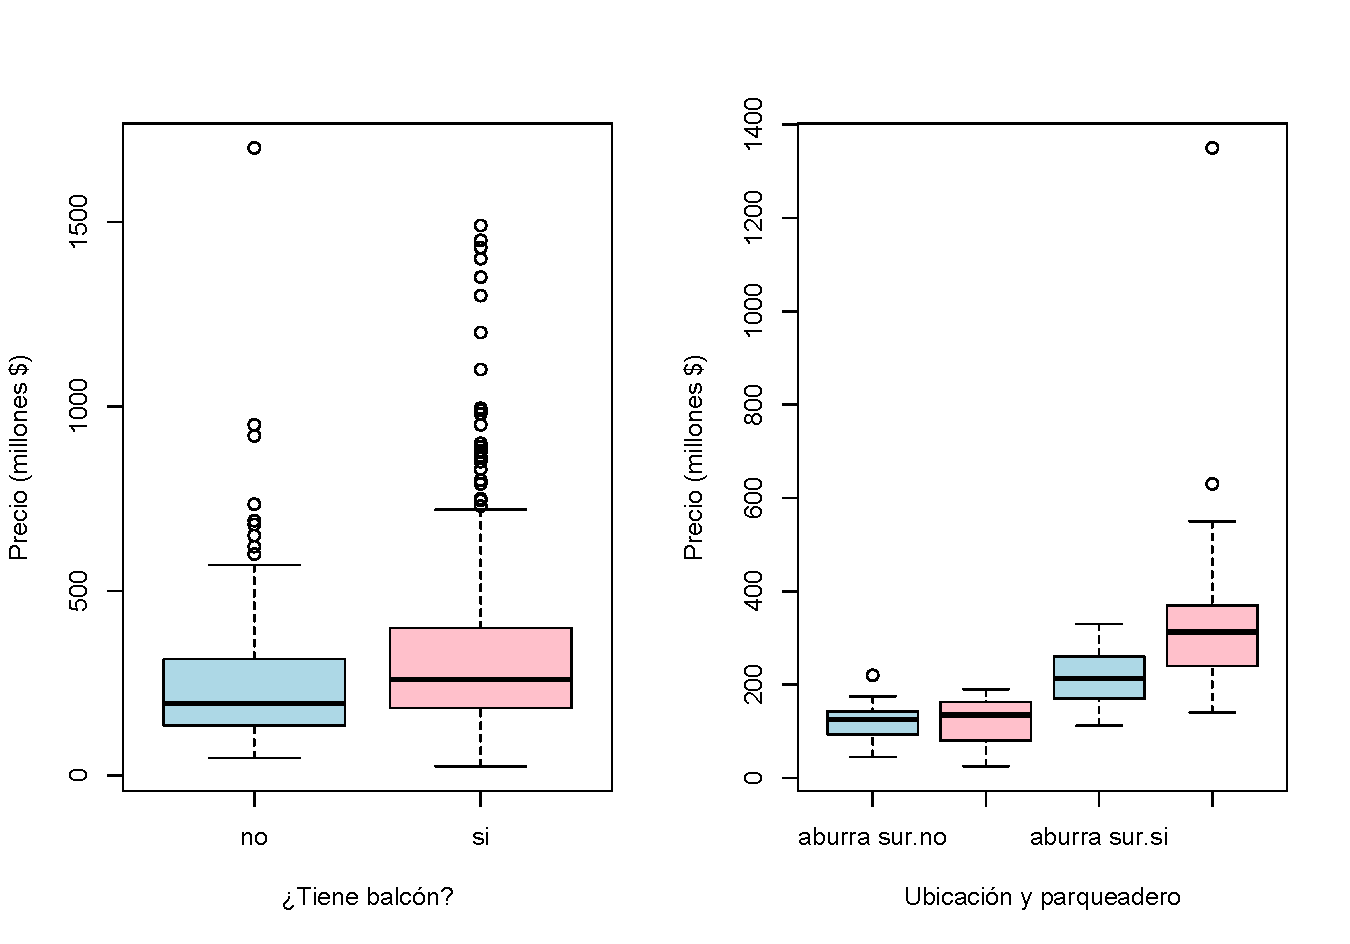
\includegraphics{Graficos_con_R_files/figure-latex/boxplots2-1.pdf}
\caption{\label{fig:boxplots2}Boxplot para la variable precio del
apartamento. En el pánel (a) de condiciona por la variable balcón y en
el pánel (b) por las combinaciones de las variables ubicación y
parqueadero.}
\end{figure}

En la Figura \ref{fig:boxplots2} se muestran los boxplots. Se le
recomienda al lector construir nuevamente el segundo boxplot pero
eliminando \texttt{drop=TRUE} para que vea el efecto que tiene sobre el
dibujo.

\section{\texorpdfstring{Función
\texttt{hist}}{Función hist}}\label{funcion-hist}

La función \texttt{hist} sirve para crear el histograma
\index{histograma}\index{hist} a una variable cuantitativa. Como
argumentos esta función recibe un vector con los datos y opcionalmente
puede ingresarse como argumento adicional el número de intervalos a ser
graficados o en su defecto el número de intervalos se determina con la
fórmula de Sturges.

\BeginKnitrBlock{rmdtip}
Los programas de computador usualmente construyen los histogramas
automáticamente, sin embargo, un buen programa debe permitirnos elegir
el número de intervalos del histograma. Si usted posee un programa que
no le permite hacer cambios, cambie de programa.
\EndKnitrBlock{rmdtip}

La estructura de la función \texttt{hist} con los argumentos más comunes
de uso se muestran a continuación.

\begin{itemize}
\tightlist
\item
  \texttt{x}: vector numérico de valores para construir el histograma.
\item
  \texttt{breaks}: puede ser un número entero que indica el número
  aproximado de clases o un vector cuyos elementos indican los límites
  de los intervalos.
\item
  \texttt{freq}: argumento lógico; si se especifica como \texttt{TRUE},
  el histograma presentará frecuencias absolutas o conteo de datos para
  cada intervalo; si se especifica como \texttt{FALSE} el histograma
  presentar las frecuencias relativas (en porcentaje). Por defecto, este
  argumento toma el valor de \texttt{TRUE} siempre y cuando los
  intervalos sean de igual ancho.
\item
  \texttt{include.lowest}: argumento lógico; si se especifica como
  \texttt{TRUE}, un \texttt{x{[}i{]}} igual a los equal a un valor
  \texttt{breaks} se incluirá en la primera barra, si el argumento
  \texttt{right\ =\ TRUE}, o en la última en caso contrario.
\item
  \texttt{right}: argumento lógico; si es \texttt{TRUE}, los intervalos
  son abiertos a la izquierda y cerrados a la derecha \((a,b]\). Para la
  primera clase o intervalo si \texttt{include.lowest=TRUE} el valor más
  pequeño de los datos será incluido en éste. Si es \texttt{FALSE} los
  intervalos serán de la forma \([a,b)\) y el argumento
  \texttt{include.lowest=TRUE} tendrá el significado de incluir el ``más
  alto''.
\item
  \texttt{col}: para definir el color de las barras. Por defecto,
  \texttt{NULL} produce barras sin fondo.
\item
  \texttt{border}: para definir el color de los bordes de las barras.
\item
  \texttt{plot}: argumento lógico. Por defecto es \texttt{TRUE}, y el
  resultado es el gráfico del histograma; si se especifica como
  \texttt{FALSE} el resultado es una lista de conteos por cada
  intervalo.
\item
  \texttt{labels}: argumento lógico o carácter. Si se especifica como
  \texttt{TRUE} coloca etiquetas arriba de cada barra.
\item
  \texttt{...}: parámetros gráficos adicionales a \texttt{title} y
  \texttt{axis}.
\end{itemize}

\subsection*{Ejemplo}\label{ejemplo-3}


Vamos a construir varios histogramas para los tiempos de 180 corredores
de la media maratón de CONAVI realizada hace algunos años. A
continuación se muestra la forma de ingresar los 180 datos.

\begin{Shaded}
\begin{Highlighting}[]
\NormalTok{maraton <-}\StringTok{ }\KeywordTok{c}\NormalTok{(}
\DecValTok{10253}\NormalTok{, }\DecValTok{10302}\NormalTok{, }\DecValTok{10307}\NormalTok{, }\DecValTok{10309}\NormalTok{, }\DecValTok{10349}\NormalTok{, }\DecValTok{10353}\NormalTok{, }\DecValTok{10409}\NormalTok{, }\DecValTok{10442}\NormalTok{, }\DecValTok{10447}\NormalTok{, }
\DecValTok{10452}\NormalTok{, }\DecValTok{10504}\NormalTok{, }\DecValTok{10517}\NormalTok{, }\DecValTok{10530}\NormalTok{, }\DecValTok{10540}\NormalTok{, }\DecValTok{10549}\NormalTok{, }\DecValTok{10549}\NormalTok{, }\DecValTok{10606}\NormalTok{, }\DecValTok{10612}\NormalTok{, }
\DecValTok{10646}\NormalTok{, }\DecValTok{10648}\NormalTok{, }\DecValTok{10655}\NormalTok{, }\DecValTok{10707}\NormalTok{, }\DecValTok{10726}\NormalTok{, }\DecValTok{10731}\NormalTok{, }\DecValTok{10737}\NormalTok{, }\DecValTok{10743}\NormalTok{, }\DecValTok{10808}\NormalTok{, }
\DecValTok{10833}\NormalTok{, }\DecValTok{10843}\NormalTok{, }\DecValTok{10920}\NormalTok{, }\DecValTok{10938}\NormalTok{, }\DecValTok{10949}\NormalTok{, }\DecValTok{10954}\NormalTok{, }\DecValTok{10956}\NormalTok{, }\DecValTok{10958}\NormalTok{, }\DecValTok{11004}\NormalTok{, }
\DecValTok{11009}\NormalTok{, }\DecValTok{11024}\NormalTok{, }\DecValTok{11037}\NormalTok{, }\DecValTok{11045}\NormalTok{, }\DecValTok{11046}\NormalTok{, }\DecValTok{11049}\NormalTok{, }\DecValTok{11104}\NormalTok{, }\DecValTok{11127}\NormalTok{, }\DecValTok{11205}\NormalTok{, }
\DecValTok{11207}\NormalTok{, }\DecValTok{11215}\NormalTok{, }\DecValTok{11226}\NormalTok{, }\DecValTok{11233}\NormalTok{, }\DecValTok{11239}\NormalTok{, }\DecValTok{11307}\NormalTok{, }\DecValTok{11330}\NormalTok{, }\DecValTok{11342}\NormalTok{, }\DecValTok{11351}\NormalTok{, }
\DecValTok{11405}\NormalTok{, }\DecValTok{11413}\NormalTok{, }\DecValTok{11438}\NormalTok{, }\DecValTok{11453}\NormalTok{, }\DecValTok{11500}\NormalTok{, }\DecValTok{11501}\NormalTok{, }\DecValTok{11502}\NormalTok{, }\DecValTok{11503}\NormalTok{, }\DecValTok{11527}\NormalTok{, }
\DecValTok{11544}\NormalTok{, }\DecValTok{11549}\NormalTok{, }\DecValTok{11559}\NormalTok{, }\DecValTok{11612}\NormalTok{, }\DecValTok{11617}\NormalTok{, }\DecValTok{11635}\NormalTok{, }\DecValTok{11655}\NormalTok{, }\DecValTok{11731}\NormalTok{, }\DecValTok{11735}\NormalTok{,}
\DecValTok{11746}\NormalTok{, }\DecValTok{11800}\NormalTok{, }\DecValTok{11814}\NormalTok{, }\DecValTok{11828}\NormalTok{, }\DecValTok{11832}\NormalTok{, }\DecValTok{11841}\NormalTok{, }\DecValTok{11909}\NormalTok{, }\DecValTok{11926}\NormalTok{, }\DecValTok{11937}\NormalTok{, }
\DecValTok{11940}\NormalTok{, }\DecValTok{11947}\NormalTok{, }\DecValTok{11952}\NormalTok{, }\DecValTok{12005}\NormalTok{, }\DecValTok{12044}\NormalTok{, }\DecValTok{12113}\NormalTok{, }\DecValTok{12209}\NormalTok{, }\DecValTok{12230}\NormalTok{, }\DecValTok{12258}\NormalTok{, }
\DecValTok{12309}\NormalTok{, }\DecValTok{12327}\NormalTok{, }\DecValTok{12341}\NormalTok{, }\DecValTok{12413}\NormalTok{, }\DecValTok{12433}\NormalTok{, }\DecValTok{12440}\NormalTok{, }\DecValTok{12447}\NormalTok{, }\DecValTok{12530}\NormalTok{, }\DecValTok{12600}\NormalTok{, }
\DecValTok{12617}\NormalTok{, }\DecValTok{12640}\NormalTok{, }\DecValTok{12700}\NormalTok{, }\DecValTok{12706}\NormalTok{, }\DecValTok{12727}\NormalTok{, }\DecValTok{12840}\NormalTok{, }\DecValTok{12851}\NormalTok{, }\DecValTok{12851}\NormalTok{, }\DecValTok{12937}\NormalTok{,}
\DecValTok{13019}\NormalTok{, }\DecValTok{13040}\NormalTok{, }\DecValTok{13110}\NormalTok{, }\DecValTok{13114}\NormalTok{, }\DecValTok{13122}\NormalTok{, }\DecValTok{13155}\NormalTok{, }\DecValTok{13205}\NormalTok{, }\DecValTok{13210}\NormalTok{, }\DecValTok{13220}\NormalTok{, }
\DecValTok{13228}\NormalTok{, }\DecValTok{13307}\NormalTok{, }\DecValTok{13316}\NormalTok{, }\DecValTok{13335}\NormalTok{, }\DecValTok{13420}\NormalTok{, }\DecValTok{13425}\NormalTok{, }\DecValTok{13435}\NormalTok{, }\DecValTok{13435}\NormalTok{, }\DecValTok{13448}\NormalTok{, }
\DecValTok{13456}\NormalTok{, }\DecValTok{13536}\NormalTok{, }\DecValTok{13608}\NormalTok{, }\DecValTok{13612}\NormalTok{, }\DecValTok{13620}\NormalTok{, }\DecValTok{13646}\NormalTok{, }\DecValTok{13705}\NormalTok{, }\DecValTok{13730}\NormalTok{, }\DecValTok{13730}\NormalTok{, }
\DecValTok{13730}\NormalTok{, }\DecValTok{13747}\NormalTok{, }\DecValTok{13810}\NormalTok{, }\DecValTok{13850}\NormalTok{, }\DecValTok{13854}\NormalTok{, }\DecValTok{13901}\NormalTok{, }\DecValTok{13905}\NormalTok{, }\DecValTok{13907}\NormalTok{, }\DecValTok{13912}\NormalTok{,}
\DecValTok{13920}\NormalTok{, }\DecValTok{14000}\NormalTok{, }\DecValTok{14010}\NormalTok{, }\DecValTok{14025}\NormalTok{, }\DecValTok{14152}\NormalTok{, }\DecValTok{14208}\NormalTok{, }\DecValTok{14230}\NormalTok{, }\DecValTok{14344}\NormalTok{, }\DecValTok{14400}\NormalTok{, }
\DecValTok{14455}\NormalTok{, }\DecValTok{14509}\NormalTok{, }\DecValTok{14552}\NormalTok{, }\DecValTok{14652}\NormalTok{, }\DecValTok{15009}\NormalTok{, }\DecValTok{15026}\NormalTok{, }\DecValTok{15242}\NormalTok{, }\DecValTok{15406}\NormalTok{, }\DecValTok{15409}\NormalTok{, }
\DecValTok{15528}\NormalTok{, }\DecValTok{15549}\NormalTok{, }\DecValTok{15644}\NormalTok{, }\DecValTok{15758}\NormalTok{, }\DecValTok{15837}\NormalTok{, }\DecValTok{15916}\NormalTok{, }\DecValTok{15926}\NormalTok{, }\DecValTok{15948}\NormalTok{, }\DecValTok{20055}\NormalTok{, }
\DecValTok{20416}\NormalTok{, }\DecValTok{20520}\NormalTok{, }\DecValTok{20600}\NormalTok{, }\DecValTok{20732}\NormalTok{, }\DecValTok{20748}\NormalTok{, }\DecValTok{20916}\NormalTok{, }\DecValTok{21149}\NormalTok{, }\DecValTok{21714}\NormalTok{, }\DecValTok{23256}\NormalTok{)}
\end{Highlighting}
\end{Shaded}

Los datos están codificados como por seis números en el formato hmmss,
donde h corresponde a las horas, mm a los minutos y ss a los segundos
necesarios para completar la maratón. Antes de construir los histogramas
es necesario convertir los tiempos anteriores almacenados en
\texttt{maraton} a horas, para esto se utiliza el siguiente código.

\begin{Shaded}
\begin{Highlighting}[]
\NormalTok{horas <-}\StringTok{ }\NormalTok{maraton }\OperatorTok\StringTok{ }\DecValTok{10000}
\NormalTok{min <-}\StringTok{ }\NormalTok{(maraton }\OperatorTok{-}\StringTok{ }\NormalTok{horas }\OperatorTok{*}\StringTok{ }\DecValTok{10000}\NormalTok{) }\OperatorTok\StringTok{ }\DecValTok{100}
\NormalTok{seg <-}\StringTok{ }\NormalTok{maraton }\OperatorTok{-}\StringTok{ }\NormalTok{horas }\OperatorTok{*}\StringTok{ }\DecValTok{10000} \OperatorTok{-}\StringTok{ }\NormalTok{min }\OperatorTok{*}\StringTok{ }\DecValTok{100}
\NormalTok{Tiempos <-}\StringTok{ }\NormalTok{horas }\OperatorTok{+}\StringTok{ }\NormalTok{min }\OperatorTok{/}\StringTok{ }\DecValTok{60} \OperatorTok{+}\StringTok{ }\NormalTok{seg }\OperatorTok{/}\StringTok{ }\DecValTok{3600}
\end{Highlighting}
\end{Shaded}

A continuación se muestra el código para construir cuatro histogramas
con 2, 4, 8 y 16 intervalos para los tiempos a partir de la variable
\texttt{Tiempos}.

\begin{Shaded}
\begin{Highlighting}[]
\KeywordTok{par}\NormalTok{(}\DataTypeTok{mfrow=}\KeywordTok{c}\NormalTok{(}\DecValTok{2}\NormalTok{,}\DecValTok{2}\NormalTok{))}

\KeywordTok{hist}\NormalTok{(}\DataTypeTok{x=}\NormalTok{Tiempos, }\DataTypeTok{breaks=}\DecValTok{2}\NormalTok{, }\DataTypeTok{main=}\StringTok{""}\NormalTok{, }\DataTypeTok{xlab=}\StringTok{"Tiempo (horas)"}\NormalTok{,}
     \DataTypeTok{ylab=}\StringTok{"Frecuencias"}\NormalTok{, }\DataTypeTok{las=}\DecValTok{1}\NormalTok{)}
\KeywordTok{mtext}\NormalTok{(}\StringTok{"(A)"}\NormalTok{, }\DataTypeTok{side=}\DecValTok{1}\NormalTok{, }\DataTypeTok{line=}\DecValTok{4}\NormalTok{, }\DataTypeTok{font=}\DecValTok{1}\NormalTok{)}

\KeywordTok{hist}\NormalTok{(}\DataTypeTok{x=}\NormalTok{Tiempos, }\DataTypeTok{breaks=}\DecValTok{4}\NormalTok{, }\DataTypeTok{main=}\StringTok{""}\NormalTok{, }\DataTypeTok{xlab=}\StringTok{"Tiempo (horas)"}\NormalTok{,}
     \DataTypeTok{ylab=}\StringTok{"Frecuencias"}\NormalTok{, }\DataTypeTok{las=}\DecValTok{1}\NormalTok{)}
\KeywordTok{mtext}\NormalTok{(}\StringTok{"(B)"}\NormalTok{, }\DataTypeTok{side=}\DecValTok{1}\NormalTok{, }\DataTypeTok{line=}\DecValTok{4}\NormalTok{, }\DataTypeTok{font=}\DecValTok{1}\NormalTok{)}

\KeywordTok{hist}\NormalTok{(}\DataTypeTok{x=}\NormalTok{Tiempos, }\DataTypeTok{breaks=}\DecValTok{8}\NormalTok{, }\DataTypeTok{main=}\StringTok{""}\NormalTok{, }\DataTypeTok{xlab=}\StringTok{"Tiempo (horas)"}\NormalTok{,}
     \DataTypeTok{ylab=}\StringTok{"Frecuencias"}\NormalTok{)}
\KeywordTok{mtext}\NormalTok{(}\StringTok{"(C)"}\NormalTok{, }\DataTypeTok{side=}\DecValTok{1}\NormalTok{, }\DataTypeTok{line=}\DecValTok{4}\NormalTok{, }\DataTypeTok{font=}\DecValTok{1}\NormalTok{)}

\KeywordTok{hist}\NormalTok{(}\DataTypeTok{x=}\NormalTok{Tiempos, }\DataTypeTok{breaks=}\DecValTok{16}\NormalTok{, }\DataTypeTok{main=}\StringTok{""}\NormalTok{, }\DataTypeTok{xlab=}\StringTok{"Tiempo (horas)"}\NormalTok{,}
     \DataTypeTok{ylab=}\StringTok{"Frecuencias"}\NormalTok{)}
\KeywordTok{mtext}\NormalTok{(}\StringTok{"(D)"}\NormalTok{, }\DataTypeTok{side=}\DecValTok{1}\NormalTok{, }\DataTypeTok{line=}\DecValTok{4}\NormalTok{, }\DataTypeTok{font=}\DecValTok{1}\NormalTok{)}
\end{Highlighting}
\end{Shaded}

\begin{figure}
\centering
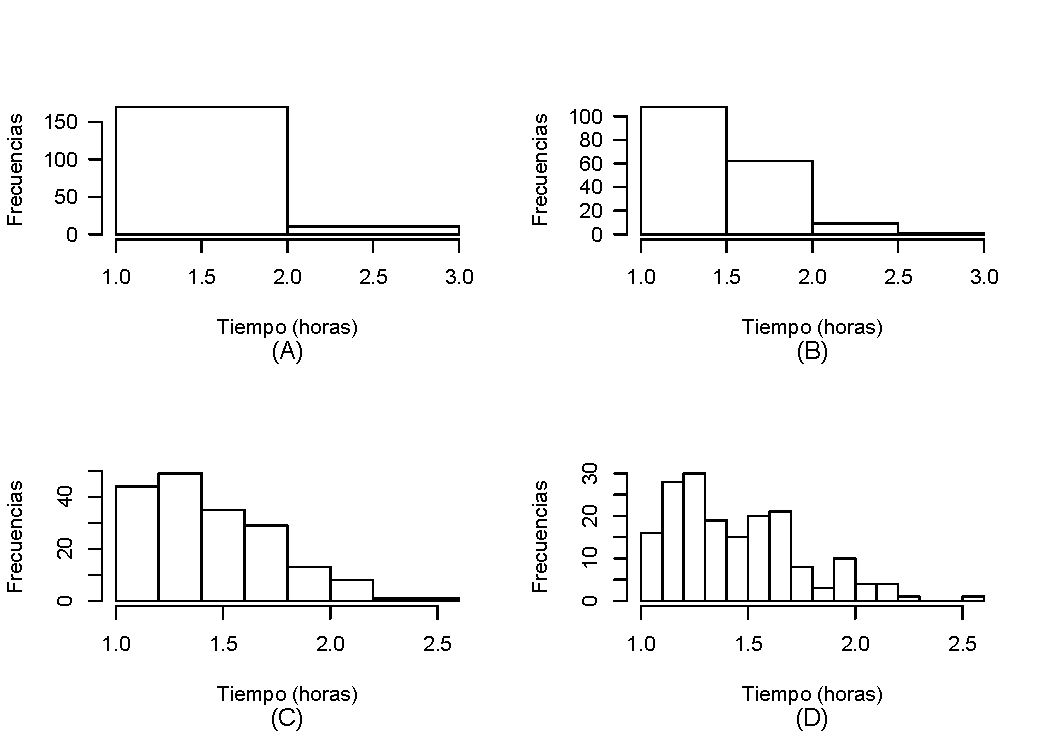
\includegraphics{Graficos_con_R_files/figure-latex/hist1-1.pdf}
\caption{\label{fig:hist1}Histogramas para el tiempo en la media maratón de
CONAVI. A: histograma con dos intervalos, B: histograma con cuatro
intervalos, C: histograma con seis intervalos, C: histograma con 18
intervalos.}
\end{figure}

En la Figura \ref{fig:hist1} se presentan los cuatro histogramas. El
histograma C, con 8 barras, muestra más claramente la asimetría (este es
el que la mayoría de los programas produce por defecto, ya que la regla
de Sturges para este conjunto de datos aproxima a 8 barras). Si
consideramos más barras por ejemplo 16, como tenemos en D, se refina más
la información y empezamos a notar multimodalidad. En el código anterior
se incluyó \texttt{las\ =\ 1} para conseguir que los número del eje Y
queden escritos de forma horizontal, ver A y B en Figura
\ref{fig:hist1}.

A continuación vamos a construir cuatro histogramas: el primero con dos
intervalos intervalos y puntos de corte dados por el mínimo, la mediana
y el máximo; el segundo con tres intervalos y puntos de corte dados por
el mínimo, cuartiles 1, 2, 3 y máximo; el cuarto con diez intervalos y
puntos de corte dados por los deciles; y el último con veinte intervalos
y puntos de corte dados por cuantiles 5, 10, \(\ldots\), 95. En el
código mostrado a continuación se presenta la creación de los puntos de
corte y los cuatro histogramas.

\begin{Shaded}
\begin{Highlighting}[]
\NormalTok{puntos1 <-}\StringTok{ }\KeywordTok{c}\NormalTok{(}\KeywordTok{quantile}\NormalTok{(Tiempos, }\DataTypeTok{probs=}\KeywordTok{c}\NormalTok{(}\DecValTok{0}\NormalTok{, }\FloatTok{0.5}\NormalTok{, }\DecValTok{1}\NormalTok{)))}
\NormalTok{puntos2 <-}\StringTok{ }\KeywordTok{c}\NormalTok{(}\KeywordTok{quantile}\NormalTok{(Tiempos, }\DataTypeTok{probs=}\KeywordTok{c}\NormalTok{(}\DecValTok{0}\NormalTok{, }\FloatTok{0.25}\NormalTok{, }\FloatTok{0.5}\NormalTok{, }\FloatTok{0.75}\NormalTok{, }\DecValTok{1}\NormalTok{)))}
\NormalTok{puntos3 <-}\StringTok{ }\KeywordTok{c}\NormalTok{(}\KeywordTok{quantile}\NormalTok{(Tiempos, }\DataTypeTok{probs=}\KeywordTok{seq}\NormalTok{(}\DecValTok{0}\NormalTok{, }\DecValTok{1}\NormalTok{, }\DataTypeTok{by=}\FloatTok{0.1}\NormalTok{)))}
\NormalTok{puntos4 <-}\StringTok{ }\KeywordTok{c}\NormalTok{(}\KeywordTok{quantile}\NormalTok{(Tiempos, }\DataTypeTok{probs=}\KeywordTok{seq}\NormalTok{(}\DecValTok{0}\NormalTok{, }\DecValTok{1}\NormalTok{, }\DataTypeTok{by=}\FloatTok{0.05}\NormalTok{)))}

\KeywordTok{par}\NormalTok{(}\DataTypeTok{mfrow=}\KeywordTok{c}\NormalTok{(}\DecValTok{2}\NormalTok{, }\DecValTok{2}\NormalTok{))}
\KeywordTok{hist}\NormalTok{(Tiempos, }\DataTypeTok{breaks=}\NormalTok{puntos1, }\DataTypeTok{freq=}\OtherTok{FALSE}\NormalTok{, }\DataTypeTok{ylim=}\KeywordTok{c}\NormalTok{(}\DecValTok{0}\NormalTok{,}\DecValTok{2}\NormalTok{), }\DataTypeTok{labels=}\OtherTok{TRUE}\NormalTok{,}
     \DataTypeTok{main=}\StringTok{""}\NormalTok{, }\DataTypeTok{ylab=}\StringTok{"Densidad"}\NormalTok{)}
\KeywordTok{mtext}\NormalTok{(}\StringTok{"(A)"}\NormalTok{, }\DataTypeTok{side=}\DecValTok{1}\NormalTok{, }\DataTypeTok{line=}\DecValTok{4}\NormalTok{, }\DataTypeTok{font=}\DecValTok{1}\NormalTok{)}
\KeywordTok{hist}\NormalTok{(Tiempos, }\DataTypeTok{breaks=}\NormalTok{puntos2, }\DataTypeTok{freq=}\OtherTok{FALSE}\NormalTok{, }\DataTypeTok{ylim=}\KeywordTok{c}\NormalTok{(}\DecValTok{0}\NormalTok{,}\DecValTok{2}\NormalTok{), }\DataTypeTok{labels=}\OtherTok{TRUE}\NormalTok{,}
     \DataTypeTok{main=}\StringTok{""}\NormalTok{, }\DataTypeTok{ylab=}\StringTok{"Densidad"}\NormalTok{)}
\KeywordTok{mtext}\NormalTok{(}\StringTok{"(B)"}\NormalTok{, }\DataTypeTok{side=}\DecValTok{1}\NormalTok{, }\DataTypeTok{line=}\DecValTok{4}\NormalTok{, }\DataTypeTok{font=}\DecValTok{1}\NormalTok{)}
\KeywordTok{hist}\NormalTok{(Tiempos, }\DataTypeTok{breaks=}\NormalTok{puntos3, }\DataTypeTok{freq=}\OtherTok{FALSE}\NormalTok{, }\DataTypeTok{ylim=}\KeywordTok{c}\NormalTok{(}\DecValTok{0}\NormalTok{,}\DecValTok{2}\NormalTok{),}
     \DataTypeTok{main=}\StringTok{""}\NormalTok{, }\DataTypeTok{ylab=}\StringTok{"Densidad"}\NormalTok{)}
\KeywordTok{mtext}\NormalTok{(}\StringTok{"(C)"}\NormalTok{, }\DataTypeTok{side=}\DecValTok{1}\NormalTok{, }\DataTypeTok{line=}\DecValTok{4}\NormalTok{, }\DataTypeTok{font=}\DecValTok{1}\NormalTok{)}
\KeywordTok{hist}\NormalTok{(Tiempos, }\DataTypeTok{breaks=}\NormalTok{puntos4, }\DataTypeTok{freq=}\OtherTok{FALSE}\NormalTok{, }\DataTypeTok{ylim=}\KeywordTok{c}\NormalTok{(}\DecValTok{0}\NormalTok{,}\DecValTok{2}\NormalTok{),}
     \DataTypeTok{main=}\StringTok{""}\NormalTok{, }\DataTypeTok{ylab=}\StringTok{"Densidad"}\NormalTok{)}
\KeywordTok{mtext}\NormalTok{(}\StringTok{"(D)"}\NormalTok{, }\DataTypeTok{side=}\DecValTok{1}\NormalTok{, }\DataTypeTok{line=}\DecValTok{4}\NormalTok{, }\DataTypeTok{font=}\DecValTok{1}\NormalTok{)}
\end{Highlighting}
\end{Shaded}

\begin{figure}
\centering
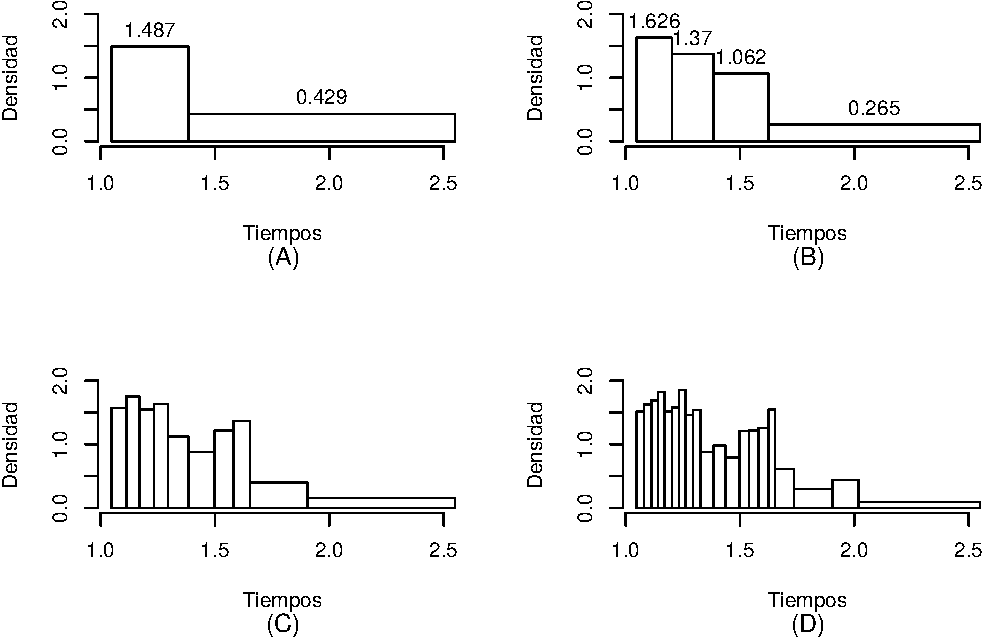
\includegraphics{Graficos_con_R_files/figure-latex/hist2-1.pdf}
\caption{\label{fig:hist2}Histogramas para el tiempo en la media maratón de
CONAVI. A: histograma con dos intervalos, B: histograma con cuatro
intervalos, C: histograma con diez intervalos, C: histograma con veinte
intervalos.}
\end{figure}

Nota: En estos histogramas, las alturas corresponden a las intensidades
(frec. relativa/long. intervalo). Por tanto, el área de cada rectángulo
da cuenta de las frecuencias relativas. Para el caso (A) ambos
intervalos tienen igual área y cada uno contiene 50\% de los datos. esto
puede verificarse así:

\begin{verbatim}
Intensidad primera clase = 1.4869888 = 0.5 / (1.384306 - 1.048056)
Intensidad segunda clase = 0.4293381 = 0.5 / (2.548889 - 1.384306)
\end{verbatim}

\section{\texorpdfstring{Función \texttt{qqnorm} y \texttt{qqplot}
\index{qqnorm}
\index{qqplot}}{Función qqnorm y qqplot  }}\label{funcion-qqnorm-y-qqplot}

Los gráficos cuantil cuantil (quantile-quantile plot) son una ayuda para
explorar si un conjunto de datos o muestra proviene de una población con
cierta distribución.

La función \texttt{qqnorm} sirve para explorar la normalidad de una
muestra mientras que la función \texttt{qqplot} es de propósito más
general, sirve para crear el gráfico cuantil cuantil para cualquier
distribución.

La estructura de las funciones con los argumentos más comunes de uso se
muestran a continuación.

\begin{Shaded}
\begin{Highlighting}[]
\KeywordTok{qqnorm}\NormalTok{(y, ...)}
\KeywordTok{qqplot}\NormalTok{(y, x, ...)}
\end{Highlighting}
\end{Shaded}

La función \texttt{qqnorm} sólo necesita que se le ingrese el vector con
la muestra por medio del parámetro \texttt{y}, la función
\texttt{qqplot} necesita de la muestra en el parámetro \texttt{y} y que
se ingrese en el parámetro \texttt{x} los cuantiles de la población
candidata.

Existe otra función útil y es \texttt{qqline}, esta función sirve para
agregar una línea de referencia al gráfico cuantil cuantil obtenido con
\texttt{qqnorm}.

\subsection*{Ejemplo}\label{ejemplo-4}


Simular 30 observaciones de una distribución \(N(\mu=10, \sigma=4)\) y
construir el gráfico cuantil cuantil.

El código para simular la muestra y crear el gráfico cuantil cuantil se
muestra a continuación.

\begin{Shaded}
\begin{Highlighting}[]
\NormalTok{muestra <-}\StringTok{ }\KeywordTok{rnorm}\NormalTok{(}\DataTypeTok{n=}\DecValTok{30}\NormalTok{, }\DataTypeTok{mean=}\DecValTok{10}\NormalTok{, }\DataTypeTok{sd=}\DecValTok{4}\NormalTok{)}

\KeywordTok{par}\NormalTok{(}\DataTypeTok{mfrow=}\KeywordTok{c}\NormalTok{(}\DecValTok{1}\NormalTok{, }\DecValTok{2}\NormalTok{))}

\KeywordTok{qqnorm}\NormalTok{(}\DataTypeTok{y=}\NormalTok{muestra)}
\KeywordTok{qqline}\NormalTok{(}\DataTypeTok{y=}\NormalTok{muestra)}

\KeywordTok{qqnorm}\NormalTok{(}\DataTypeTok{y=}\NormalTok{muestra, }\DataTypeTok{main=}\StringTok{''}\NormalTok{, }\DataTypeTok{ylab=}\StringTok{'Cuantiles muestrales'}\NormalTok{,}
       \DataTypeTok{xlab=}\StringTok{'Cuantiles teóricos', las=1)}
\StringTok{qqline(y=muestra, col='}\NormalTok{blue}\StringTok{', lwd=2, lty=2)}
\end{Highlighting}
\end{Shaded}

\begin{figure}
\centering
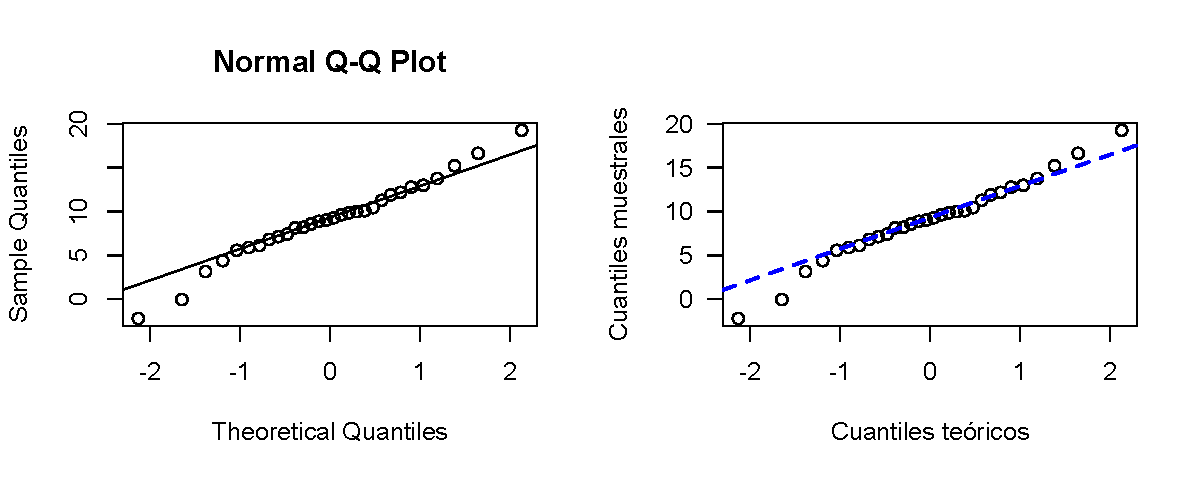
\includegraphics{Graficos_con_R_files/figure-latex/qqplot1-1.pdf}
\caption{\label{fig:qqplot1}Gráfico cuantil cuantil para una muestra
generada de una población normal.}
\end{figure}

En la izquierda de la Figura \ref{fig:qqplot1} está el gráfico cuantil
cuantil sin editar, en la derecha se encuentra el gráfico luego de
modificar los nombres de los ejes, grosor y color de la línea de
referencia.

\subsection*{Ejemplo}\label{ejemplo-5}


Simular 100 observaciones de una distribución \(Weibull(1,1)\) y
construir dos gráficos cuantil cuantil, el primero tomando como
referencia los cuantiles de una \(N(0,1)\) y el segundo tomando los
cuantiles de la \(Weibull(1,1)\).

El código para simular la muestra y crear los gráficos cuantil cuantil
se muestra a continuación.

\begin{Shaded}
\begin{Highlighting}[]
\NormalTok{n <-}\StringTok{ }\DecValTok{100}
\NormalTok{muestra <-}\StringTok{ }\KeywordTok{rweibull}\NormalTok{(}\DataTypeTok{n=}\NormalTok{n, }\DataTypeTok{shape=}\DecValTok{1}\NormalTok{, }\DataTypeTok{scale=}\DecValTok{1}\NormalTok{)}

\KeywordTok{par}\NormalTok{(}\DataTypeTok{mfrow=}\KeywordTok{c}\NormalTok{(}\DecValTok{1}\NormalTok{, }\DecValTok{2}\NormalTok{))}
\KeywordTok{qqplot}\NormalTok{(}\DataTypeTok{y=}\NormalTok{muestra, }\DataTypeTok{x=}\KeywordTok{qnorm}\NormalTok{(}\KeywordTok{ppoints}\NormalTok{(n)))}
\KeywordTok{qqplot}\NormalTok{(}\DataTypeTok{y=}\NormalTok{muestra, }\DataTypeTok{x=}\KeywordTok{qweibull}\NormalTok{(}\KeywordTok{ppoints}\NormalTok{(n), }\DataTypeTok{shape=}\DecValTok{1}\NormalTok{, }\DataTypeTok{scale=}\DecValTok{1}\NormalTok{))}
\end{Highlighting}
\end{Shaded}

\begin{figure}
\centering
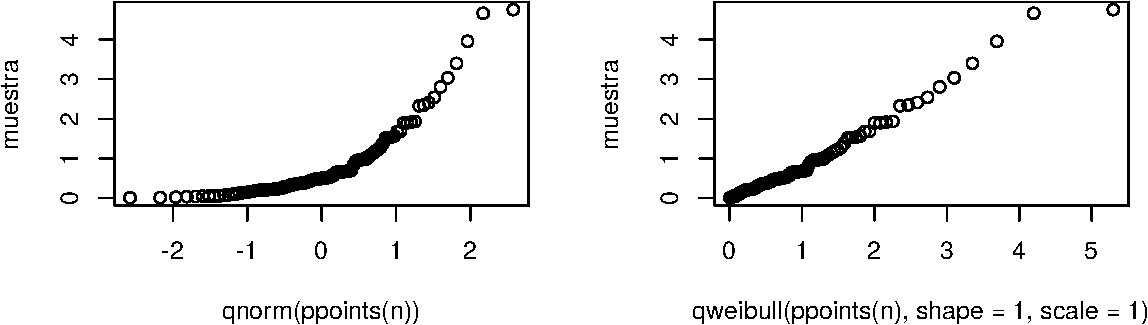
\includegraphics{Graficos_con_R_files/figure-latex/qqplot2-1.pdf}
\caption{\label{fig:qqplot2}Gráfico cuantil cuantil para una muestra
generada de una población Weibull.}
\end{figure}

En la Figura \ref{fig:qqplot2} están los gráficos cuantil cuantil
solicitados. Del pánel izquierdo de la figura vemos que los puntos NO
están alineados, esto indica que la muestra no proviene de la
distribución \(N(0, 1)\), esto es un resultado esperado ya que sabíamos
que la muestra no fue generada de una normal. En el pánel derecho de la
misma figura vemos que los puntos SI están alineados, esto indica que la
muestra generada puede provenir de una población \(Weibull(1, 1)\). Los
nombres de los ejes en la Figura \ref{fig:qqplot2} pueden ser editados
para presentar una figura con mejor apariencia.

\section{\texorpdfstring{Función \texttt{density} \index{density}
\index{densidad}}{Función density  }}\label{funcion-density}

Los gráficos de densidad son muy útiles porque permiten ver el(los)
intervalo(s) donde una variable cuantitativa puede ocurrir con mayor
probabilidad.

La función \texttt{density} crea la información de la densidad y la
función \texttt{plot} dibuja la densidad.

La estructura de la función \texttt{density} con los argumentos más
comunes de uso se muestra a continuación.

\begin{Shaded}
\begin{Highlighting}[]
\KeywordTok{density}\NormalTok{(x, bw, }\DataTypeTok{adjust=}\DecValTok{1}\NormalTok{, }\DataTypeTok{kernel=}\StringTok{'gaussian'}\NormalTok{, }\DataTypeTok{na.rm=}\OtherTok{FALSE}\NormalTok{)}
\end{Highlighting}
\end{Shaded}

Los argumentos de la función \texttt{density} son:

\begin{itemize}
\tightlist
\item
  \texttt{x}: vector con los datos para los cuales se quiere la
  densidad.
\item
  \texttt{bw}: ancho de banda.
\item
  \texttt{kernel}: núcleo de suavización a usar, los posibles valores
  son \texttt{gaussian}, \texttt{rectangular}, \texttt{triangular},
  \texttt{epanechnikov}, \texttt{biweight}, \texttt{cosine} o
  \texttt{optcosine}, el valor por defecto es \texttt{gaussian}.
\item
  \texttt{na.rm}: valor lógico, si es \texttt{TRUE} se eliminan los
  valores con \texttt{NA} para construir la densidad, el valor por
  defecto es \texttt{FALSE}.
\end{itemize}

\subsection*{Ejemplo}\label{ejemplo-6}


Simular mil observaciones de una \(N(0, 1)\), aplicar la función
\texttt{density} al vector y explorar el contenido de la salida.

Primero se generan las observaciones y se almacenan en el objeto
\texttt{y}, luego se aplica la función \texttt{density} y el resultado
se guarda en el objeto \texttt{res}, para explorar lo que almacena
\texttt{res} se usa la función \texttt{names}. A continuación el código
utilizado.

\begin{Shaded}
\begin{Highlighting}[]
\NormalTok{y <-}\StringTok{ }\KeywordTok{rnorm}\NormalTok{(}\DataTypeTok{n=}\DecValTok{1000}\NormalTok{)}
\NormalTok{res <-}\StringTok{ }\KeywordTok{density}\NormalTok{(y)}
\KeywordTok{names}\NormalTok{(res)}
\end{Highlighting}
\end{Shaded}

\begin{verbatim}
## [1] "x"         "y"         "bw"        "n"        
## [5] "call"      "data.name" "has.na"
\end{verbatim}

De la salida anterior se observa que la lista \texttt{res} tiene 7
elementos, los dos primeros son los vectores con las coordenadas para
dibujar la densidad, los restantes elementos con información adicional.

\subsection*{Ejemplo}\label{ejemplo-7}


Con los datos generados en el ejemplo anterior construir la densidad
para varios núcleo y para varios valores de ancho de banda.

En el siguiente código se construyen 4 densidades para diferentes
núcleos.

\begin{Shaded}
\begin{Highlighting}[]
\KeywordTok{par}\NormalTok{(}\DataTypeTok{mfrow=}\KeywordTok{c}\NormalTok{(}\DecValTok{2}\NormalTok{, }\DecValTok{2}\NormalTok{))}
\KeywordTok{plot}\NormalTok{(}\KeywordTok{density}\NormalTok{(y, }\DataTypeTok{kernel=}\StringTok{'gaussian'}\NormalTok{))}
\KeywordTok{plot}\NormalTok{(}\KeywordTok{density}\NormalTok{(y, }\DataTypeTok{kernel=}\StringTok{'triangular'}\NormalTok{))}
\KeywordTok{plot}\NormalTok{(}\KeywordTok{density}\NormalTok{(y, }\DataTypeTok{kernel=}\StringTok{'cosine'}\NormalTok{))}
\KeywordTok{plot}\NormalTok{(}\KeywordTok{density}\NormalTok{(y, }\DataTypeTok{kernel=}\StringTok{'rectangular'}\NormalTok{))}
\end{Highlighting}
\end{Shaded}

\begin{figure}
\centering
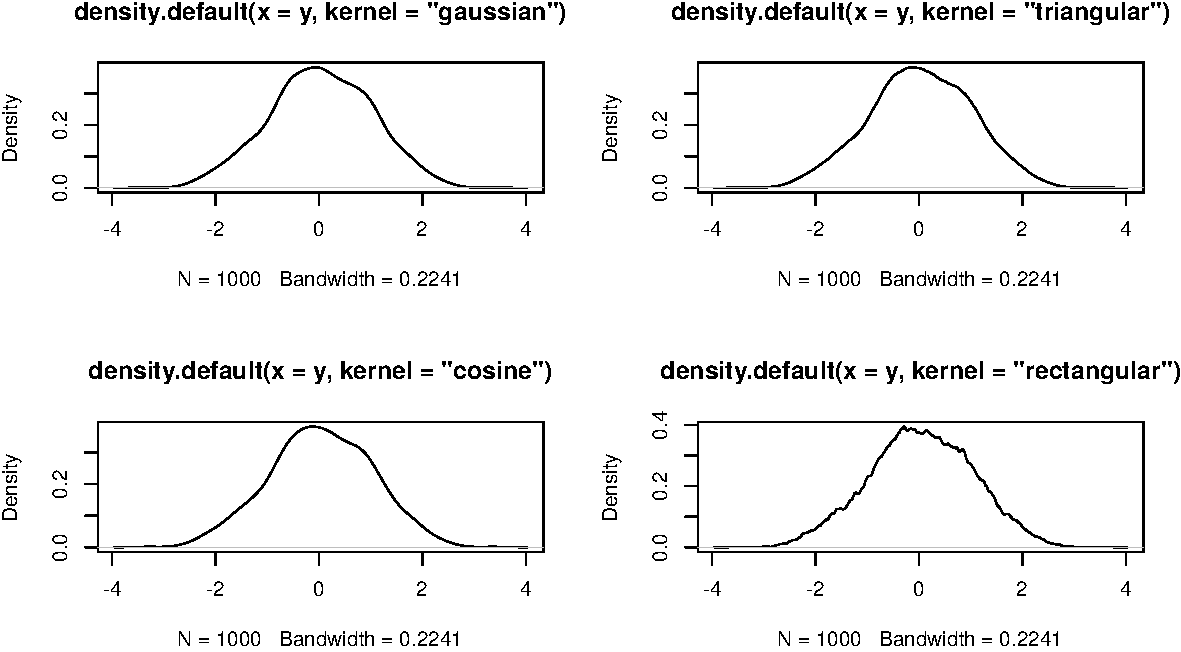
\includegraphics{Graficos_con_R_files/figure-latex/density1-1.pdf}
\caption{\label{fig:density1}Densidad para una muestra aleatoria de una N(0,
1) cambiando el núcleo de la densidad.}
\end{figure}

En la Figura \ref{fig:density1} se muestran las densidades para 4
elecciones del núcleo. En la práctica se usa el núcleo que está por
defecto (\texttt{gaussian}) ya que el objetivo de una densidad es ver la
zonas donde es más probable encontrar observaciones de la variable.

En el siguiente código se construyen 4 densidades para diferentes anchos
de banda.

\begin{Shaded}
\begin{Highlighting}[]
\KeywordTok{par}\NormalTok{(}\DataTypeTok{mfrow=}\KeywordTok{c}\NormalTok{(}\DecValTok{2}\NormalTok{, }\DecValTok{2}\NormalTok{))}
\KeywordTok{plot}\NormalTok{(}\KeywordTok{density}\NormalTok{(y, }\DataTypeTok{bw=}\FloatTok{0.1}\NormalTok{))}
\KeywordTok{plot}\NormalTok{(}\KeywordTok{density}\NormalTok{(y, }\DataTypeTok{bw=}\FloatTok{0.2241}\NormalTok{))  }\CommentTok{# bw obtenido antes}
\KeywordTok{plot}\NormalTok{(}\KeywordTok{density}\NormalTok{(y, }\DataTypeTok{bw=}\FloatTok{0.5}\NormalTok{))}
\KeywordTok{plot}\NormalTok{(}\KeywordTok{density}\NormalTok{(y, }\DataTypeTok{bw=}\DecValTok{1}\NormalTok{))}
\end{Highlighting}
\end{Shaded}

\begin{figure}
\centering
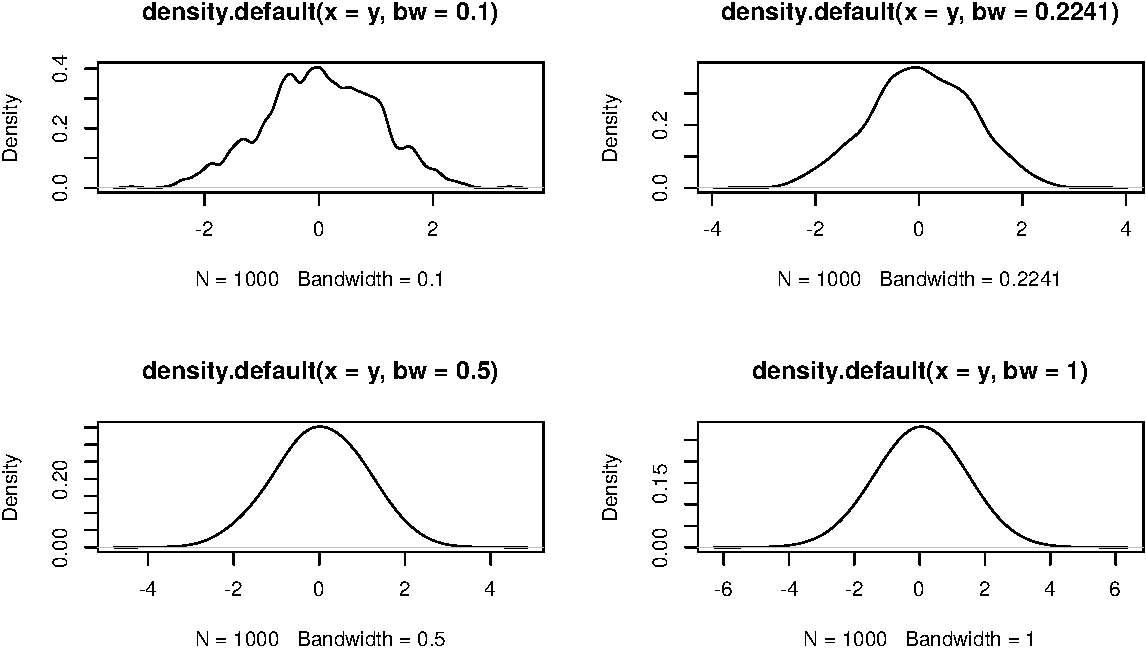
\includegraphics{Graficos_con_R_files/figure-latex/density2-1.pdf}
\caption{\label{fig:density2}Densidad para una muestra aleatoria de una N(0,
1) cambiando el ancho de banda.}
\end{figure}

En la Figura \ref{fig:density2} se muestran las densidades para 4
elecciones del parámetro ancho de banda \texttt{bw}, el valor de 0.2241
fue el valor calculado automáticamente por \proglang{R} y fue obtenido
de la Figura \ref{fig:density1}, los otros valores fueron elegidos
arbitrariamente para ver los cambios en la densidad. El usar un ancho de
banda pequeño la densidad queda muy rugosa y usar un valor muy grande la
suaviza, se recomienda usar el valor automático.

\subsection*{Ejemplo}\label{ejemplo-8}


Construir un gráfico de densidad para la variable peso corporal de la
base de datos \texttt{medidas\_cuerpo}, luego construir la densidad para
la misma variable pero diferenciando por sexo.

\begin{Shaded}
\begin{Highlighting}[]
\NormalTok{url <-}\StringTok{ 'https://raw.githubusercontent.com/fhernanb/datos/master/medidas_cuerpo'}
\NormalTok{datos <-}\StringTok{ }\KeywordTok{read.table}\NormalTok{(}\DataTypeTok{file=}\NormalTok{url, }\DataTypeTok{header=}\NormalTok{T)}

\KeywordTok{par}\NormalTok{(}\DataTypeTok{mfrow=}\KeywordTok{c}\NormalTok{(}\DecValTok{1}\NormalTok{, }\DecValTok{2}\NormalTok{))}
\KeywordTok{plot}\NormalTok{(}\KeywordTok{density}\NormalTok{(datos}\OperatorTok{$}\NormalTok{peso), }\DataTypeTok{main=}\StringTok{'Distribución del peso corporal'}\NormalTok{,}
     \DataTypeTok{xlab=}\StringTok{'Peso corporal (kg)'}\NormalTok{, }\DataTypeTok{ylab=}\StringTok{'Densidad'}\NormalTok{, }\DataTypeTok{lwd=}\DecValTok{4}\NormalTok{)}

\NormalTok{den.hom <-}\StringTok{ }\KeywordTok{with}\NormalTok{(datos, }\KeywordTok{density}\NormalTok{(peso[sexo }\OperatorTok{==}\StringTok{ 'Hombre'}\NormalTok{]))}
\NormalTok{den.muj <-}\StringTok{ }\KeywordTok{with}\NormalTok{(datos, }\KeywordTok{density}\NormalTok{(peso[sexo }\OperatorTok{==}\StringTok{ 'Mujer'}\NormalTok{]))}

\KeywordTok{plot}\NormalTok{(den.hom, }\DataTypeTok{xlim=}\KeywordTok{c}\NormalTok{(}\DecValTok{20}\NormalTok{, }\DecValTok{120}\NormalTok{), }
     \DataTypeTok{main=}\StringTok{'Distribución del peso corporal por género'}\NormalTok{, }\DataTypeTok{ylab=}\StringTok{'Densidad'}\NormalTok{,}
     \DataTypeTok{xlab=}\StringTok{'Peso corporal (kg)'}\NormalTok{, }\DataTypeTok{lwd=}\DecValTok{4}\NormalTok{, }\DataTypeTok{col=}\StringTok{'blue'}\NormalTok{)}
\KeywordTok{lines}\NormalTok{(den.muj, }\DataTypeTok{lwd=}\DecValTok{4}\NormalTok{, }\DataTypeTok{col=}\StringTok{'red'}\NormalTok{)}
\KeywordTok{legend}\NormalTok{(}\StringTok{'topright'}\NormalTok{, }\DataTypeTok{legend=}\KeywordTok{c}\NormalTok{(}\StringTok{'Hombres'}\NormalTok{, }\StringTok{'Mujeres'}\NormalTok{), }\DataTypeTok{bty=}\StringTok{'n'}\NormalTok{,}
       \DataTypeTok{lwd=}\DecValTok{3}\NormalTok{, }\DataTypeTok{col=}\KeywordTok{c}\NormalTok{(}\StringTok{'blue'}\NormalTok{, }\StringTok{'red'}\NormalTok{))}
\end{Highlighting}
\end{Shaded}

\begin{figure}
\centering
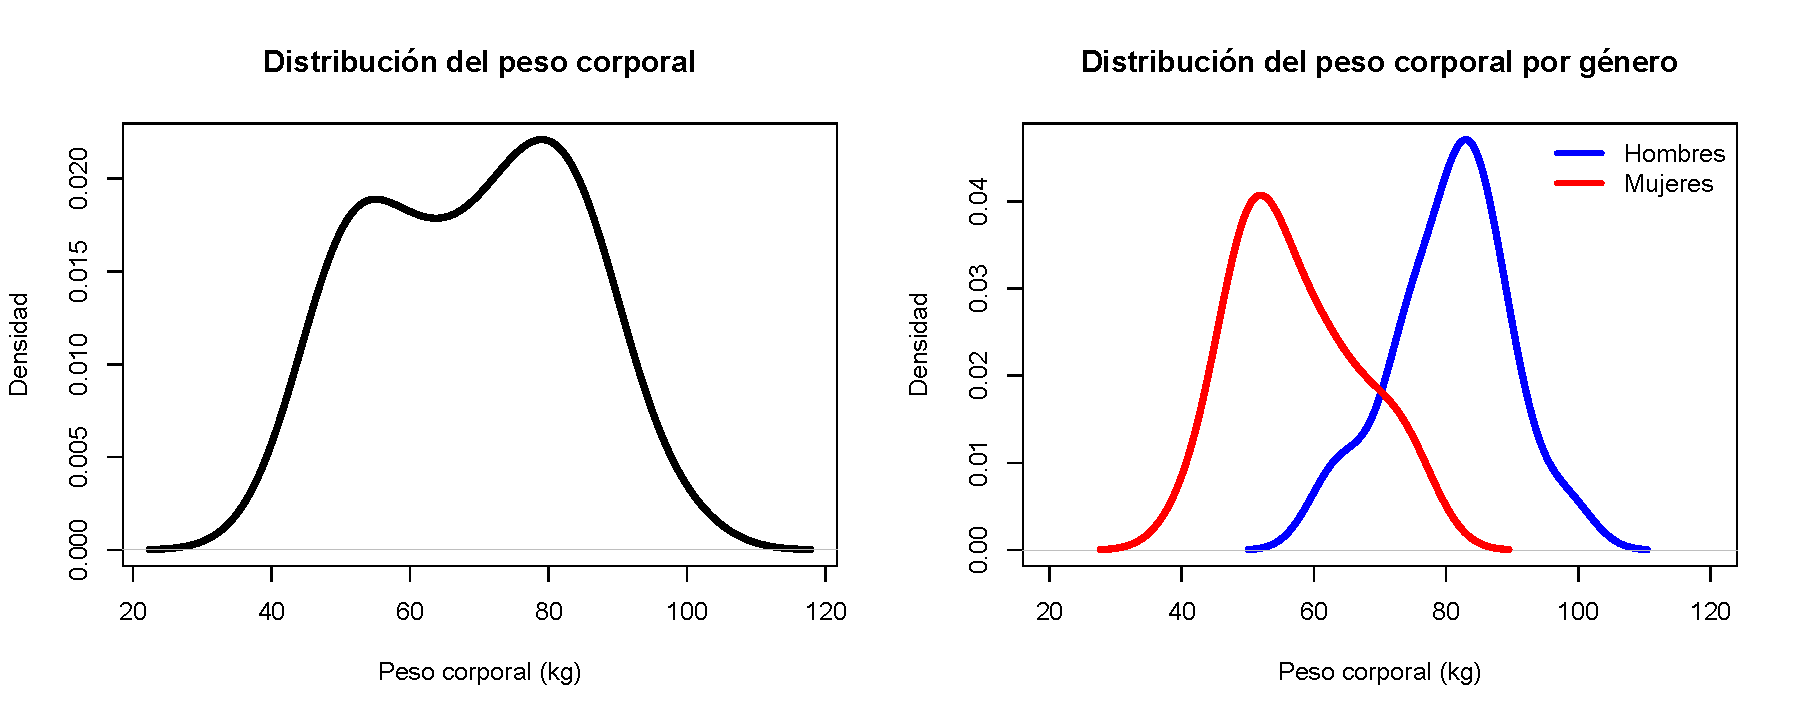
\includegraphics{Graficos_con_R_files/figure-latex/density3-1.pdf}
\caption{\label{fig:density3}Densidad para la variable peso en la izquierda,
densidad para el peso diferenciando por sexo a la derecha.}
\end{figure}

En el panel izquierdo de la Figura \ref{fig:density3} se muestra la
densidad para la variable peso, de esta figura se observa que tiene dos
sectores de mayor densidad, alrededor de 50 kg y alrededor de 80 kg. En
el panel izquierdo están la densidades del peso corporal para hombres y
mujeres, aquí se observa claramente la diferencia entre los pesos de
hombres y mujeres.

\chapter{Gráficos para varias variables
cuantitativas}\label{graficos-para-varias-variables-cuantitativas}

En este capítulo se presentan funciones para la creación de gráficos que
involucran varias variables.

\section{\texorpdfstring{Función \texttt{plot} \index{plot}
\index{diagrama de dispersión}}{Función plot  }}\label{funcion-plot}

Los gráficos de dispersión son muy útiles porque permiten ver la
relación que existe entre dos variables cuantitativas, la función
\texttt{plot} permite crear este tipo de gráficos. La estructura de la
función \texttt{plot} con los argumentos más usuales se muestra a
continuación:

\begin{Shaded}
\begin{Highlighting}[]
\KeywordTok{plot}\NormalTok{(x, y, type, main, sub, xlab, ylab)}
\end{Highlighting}
\end{Shaded}

Los argumentos de la función \texttt{plot} son:

\begin{itemize}
\tightlist
\item
  \texttt{x}: vector numérico con las coordenadas del eje horizontal.
\item
  \texttt{y}: vector numérico con las coordenadas del eje vertical.
\item
  \texttt{type}: tipo de gráfico a dibujar. Las opciones son:
  \label{type}

  \begin{itemize}
  \tightlist
  \item
    \texttt{\textquotesingle{}p\textquotesingle{}} para obtener puntos,
    esta es la opción por defecto.
  \item
    \texttt{\textquotesingle{}l\textquotesingle{}} para obtener líneas.
  \item
    \texttt{\textquotesingle{}b\textquotesingle{}} para obtener los
    puntos y líneas que unen los puntos.
  \item
    \texttt{\textquotesingle{}c\textquotesingle{}} para obtener sólo las
    líneas y dejando los espacios donde estaban los puntos obtenidos con
    la opción \texttt{\textquotesingle{}b\textquotesingle{}}.
  \item
    \texttt{\textquotesingle{}o\textquotesingle{}} para obtener los
    puntos y lineas superpuestas.
  \item
    \texttt{\textquotesingle{}h\textquotesingle{}} para obtener líneas
    verticales desde el origen hasta el valor \(y_i\) de cada punto,
    similar a un histograma.
  \item
    \texttt{\textquotesingle{}s\textquotesingle{}} para obtener
    escalones.
  \item
    \texttt{\textquotesingle{}S\textquotesingle{}} similar al anterior.
  \item
    \texttt{\textquotesingle{}n\textquotesingle{}} para que no dibuje.
  \end{itemize}
\item
  \texttt{...}: otros parámetros gráficos que pueden ser pasados como
  argumentos para \texttt{plot}.
\end{itemize}

\subsection*{Ejemplo}\label{ejemplo-9}


Crear 16 parejas de puntos tales que \(x=-5, -4, \ldots, 9, 10\) con
\(y=-10+(x-3)^2\), dibujar los nueve diagramas de dispersión de \(y\)
contra \(x\) usando todos los valores posibles para el parámetro
\texttt{type}.

A continuación se muestra el código para crear las 16 parejas de \(x\) e
\(y\). Los nueve diagramas de dispersión se observan en la Figura
\ref{fig:ex1plot}, de esta figura se observa claramente el efecto que
tiene el parámetro \texttt{type} en la construcción del diagrama de
dispersión.

\begin{Shaded}
\begin{Highlighting}[]
\NormalTok{x <-}\StringTok{ }\OperatorTok{-}\DecValTok{5}\OperatorTok{:}\DecValTok{10}
\NormalTok{y <-}\StringTok{ }\OperatorTok{-}\DecValTok{10} \OperatorTok{+}\StringTok{ }\NormalTok{(x}\OperatorTok{-}\DecValTok{3}\NormalTok{)}\OperatorTok{^}\DecValTok{2}
\KeywordTok{par}\NormalTok{(}\DataTypeTok{mfrow=}\KeywordTok{c}\NormalTok{(}\DecValTok{3}\NormalTok{, }\DecValTok{3}\NormalTok{))}
\KeywordTok{plot}\NormalTok{(}\DataTypeTok{x=}\NormalTok{x, }\DataTypeTok{y=}\NormalTok{y, }\DataTypeTok{type=}\StringTok{'p'}\NormalTok{, }\DataTypeTok{main=}\StringTok{"con type='p'"}\NormalTok{)}
\KeywordTok{plot}\NormalTok{(}\DataTypeTok{x=}\NormalTok{x, }\DataTypeTok{y=}\NormalTok{y, }\DataTypeTok{type=}\StringTok{'l'}\NormalTok{, }\DataTypeTok{main=}\StringTok{"con type='l'"}\NormalTok{)}
\KeywordTok{plot}\NormalTok{(}\DataTypeTok{x=}\NormalTok{x, }\DataTypeTok{y=}\NormalTok{y, }\DataTypeTok{type=}\StringTok{'b'}\NormalTok{, }\DataTypeTok{main=}\StringTok{"con type='b'"}\NormalTok{)}
\KeywordTok{plot}\NormalTok{(}\DataTypeTok{x=}\NormalTok{x, }\DataTypeTok{y=}\NormalTok{y, }\DataTypeTok{type=}\StringTok{'c'}\NormalTok{, }\DataTypeTok{main=}\StringTok{"con type='c'"}\NormalTok{)}
\KeywordTok{plot}\NormalTok{(}\DataTypeTok{x=}\NormalTok{x, }\DataTypeTok{y=}\NormalTok{y, }\DataTypeTok{type=}\StringTok{'o'}\NormalTok{, }\DataTypeTok{main=}\StringTok{"con type='o'"}\NormalTok{)}
\KeywordTok{plot}\NormalTok{(}\DataTypeTok{x=}\NormalTok{x, }\DataTypeTok{y=}\NormalTok{y, }\DataTypeTok{type=}\StringTok{'h'}\NormalTok{, }\DataTypeTok{main=}\StringTok{"con type='h'"}\NormalTok{)}
\KeywordTok{plot}\NormalTok{(}\DataTypeTok{x=}\NormalTok{x, }\DataTypeTok{y=}\NormalTok{y, }\DataTypeTok{type=}\StringTok{'s'}\NormalTok{, }\DataTypeTok{main=}\StringTok{"con type='s'"}\NormalTok{)}
\KeywordTok{plot}\NormalTok{(}\DataTypeTok{x=}\NormalTok{x, }\DataTypeTok{y=}\NormalTok{y, }\DataTypeTok{type=}\StringTok{'S'}\NormalTok{, }\DataTypeTok{main=}\StringTok{"con type='S'"}\NormalTok{)}
\KeywordTok{plot}\NormalTok{(}\DataTypeTok{x=}\NormalTok{x, }\DataTypeTok{y=}\NormalTok{y, }\DataTypeTok{type=}\StringTok{'n'}\NormalTok{, }\DataTypeTok{main=}\StringTok{"con type='n'"}\NormalTok{)}
\end{Highlighting}
\end{Shaded}

\begin{figure}
\centering
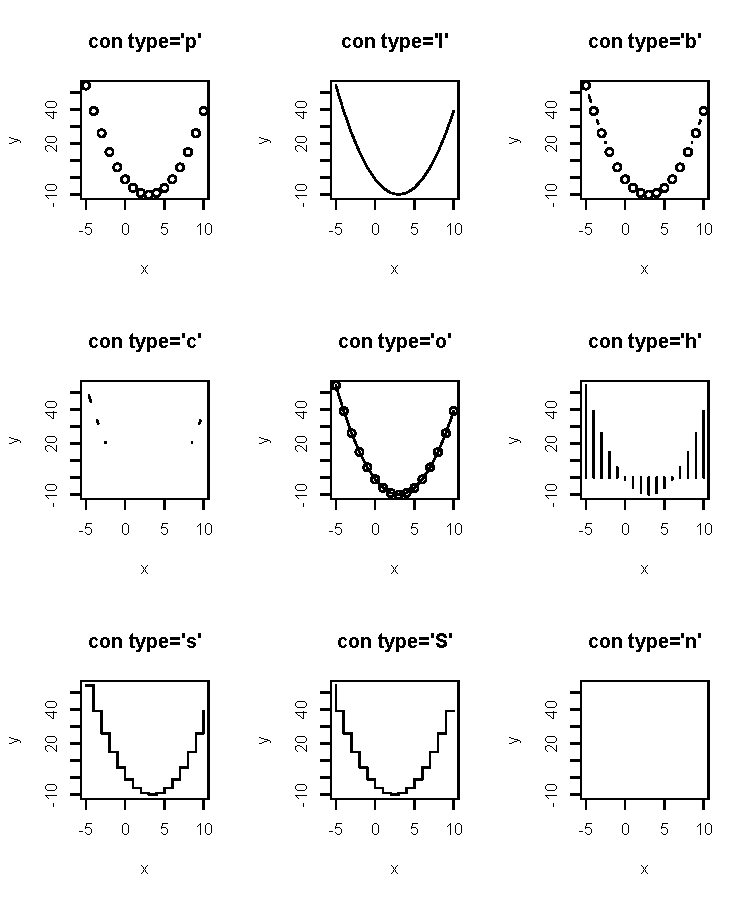
\includegraphics{Graficos_con_R_files/figure-latex/ex1plot-1.pdf}
\caption{\label{fig:ex1plot}Efecto del parámetro \texttt{type} en la función
\texttt{plot}.}
\end{figure}

\subsection*{Ejemplo}\label{ejemplo-10}


Como ilustración vamos a crear dos diagramas de dispersión entre el
precio de apartamentos usados en la ciudad de Medellín y el área de los
apartamentos. El primer diagrama es un gráfico básico mientras que el
segundo es un diagrama mejorado.

El código necesario para cargar la base de datos y construir los
diagramas de dispersión se muestra a continuación.

\begin{Shaded}
\begin{Highlighting}[]
\NormalTok{url <-}\StringTok{ 'https://tinyurl.com/hwhb769'}
\NormalTok{datos <-}\StringTok{ }\KeywordTok{read.table}\NormalTok{(}\DataTypeTok{file=}\NormalTok{url, }\DataTypeTok{header=}\NormalTok{T)}

\KeywordTok{par}\NormalTok{(}\DataTypeTok{mfrow=}\KeywordTok{c}\NormalTok{(}\DecValTok{1}\NormalTok{, }\DecValTok{2}\NormalTok{))}
\KeywordTok{plot}\NormalTok{(}\DataTypeTok{x=}\NormalTok{datos}\OperatorTok{$}\NormalTok{mt2, }\DataTypeTok{y=}\NormalTok{datos}\OperatorTok{$}\NormalTok{precio)}
\KeywordTok{plot}\NormalTok{(}\DataTypeTok{x=}\NormalTok{datos}\OperatorTok{$}\NormalTok{mt2, }\DataTypeTok{y=}\NormalTok{datos}\OperatorTok{$}\NormalTok{precio, }\DataTypeTok{pch=}\StringTok{'.'}\NormalTok{,}
     \DataTypeTok{xlab=}\StringTok{'Área del apartamento (m2)'}\NormalTok{,}
     \DataTypeTok{ylab=}\StringTok{'Precio (millones de pesos)'}\NormalTok{)}
\end{Highlighting}
\end{Shaded}

\begin{figure}
\centering
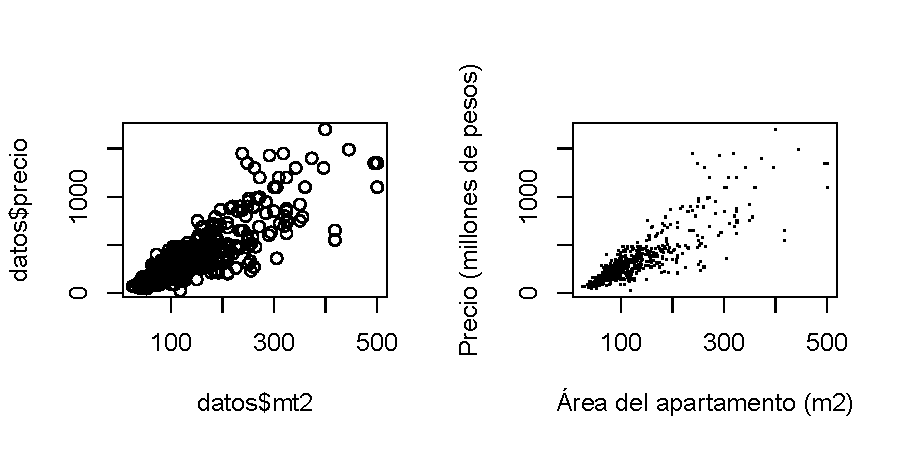
\includegraphics{Graficos_con_R_files/figure-latex/ex2plot-1.pdf}
\caption{\label{fig:ex2plot}Diagrama de dispersión del precio del
apartamento versus área del apartamento. A la izquierda el diagrama de
dispersión sin editar y a la derecha el diagrama de dispersión
mejorado.}
\end{figure}

En la Figura \ref{fig:ex2plot} se presentan los diagramas de dispersión
entre precio y área de los apartamentos. En el panel de la izquierda
está el diagrama básico, de este diagrama se observa claramente que a
medida que los apartamentos tienen mayor área el precio promedio y la
variabilidad del precio aumentan. En la parte inferior izquierda de este
diagrama se tiene una zona de alta densidad de puntos y por esa razón se
observa una mancha en el diagrama. Para la construcción del diagrama de
dispersión mostrado en el panel derecho se usó el parámetro
\texttt{pch=\textquotesingle{}.\textquotesingle{}} con el objetivo de
obtener pequeños puntos que representen cada apartamento y que no se
traslapen debido a que se tienen 694 observaciones en la base de datos.

\section{\texorpdfstring{Función \texttt{sunflowerplot}
\index{sunflowerplot}}{Función sunflowerplot }}\label{funcion-sunflowerplot}

La función \texttt{sunflowerplot} sirve para crear gráficos de
dispersión en los cuales hay parejas repetidas que se superponen y que
por lo tanto no se podrían apreciar.

Si una pareja está una sola vez se representará por un punto; si la
pareja se repite dos veces se representará por un punto y dos rayitas
rojas (pétalos); si la pareja se repite tres veces se representará por
un punto y tres rayitas rojas (pétalos) y así sucesivamente.

La estructura de la función \texttt{sunflowerplot} con los argumentos
más usuales se muestra a continuación:

\begin{Shaded}
\begin{Highlighting}[]
\KeywordTok{sunflowerplot}\NormalTok{(x, y, pch, seg.col, seg.lwd, ...)}
\end{Highlighting}
\end{Shaded}

Los argumentos de la función \texttt{plot} son:

\begin{itemize}
\tightlist
\item
  \texttt{x}: vector numérico con las coordenadas del eje horizontal.
\item
  \texttt{y}: vector numérico con las coordenadas del eje vertical.
\item
  \texttt{pch}: valor o vector numérico con el tipo de punto a usar, por
  defecto \texttt{pch=1}. Para conocer los diferentes símbolos que se
  pueden obtener con el parámetro \texttt{pch} se recomienda consultar
  la Figura \ref{fig:point1}.
\item
  \texttt{seg.col}: color de los pétalos.
\item
  \texttt{seg.lwd}: ancho de los pétalos.
\item
  \texttt{...}: otros parámetros gráficos que pueden ser pasados como
  argumentos para \texttt{plot}.
\end{itemize}

A continuación se presenta un ejemplo en los cuales se usa la función
\texttt{sunflowerplot} para crear gráficos de dispersión.

\subsection*{Ejemplo}\label{ejemplo-11}


Suponga que se tiene el punto (1, 1) una sola vez, el punto (2, 3)
repetido cuatro veces, el punto (3, 2) repetido seis veces y el punto
(4, 5) repetido dos veces. El objetivo es crear dos gráficos de
dispersión con los trece puntos, uno con la función \texttt{plot} y el
otro con la función \texttt{sunflowerplot} para comparar los resultados.

A continuación se muestra el código con la creación de los vectores y
los dos gráficos de dispersión con \texttt{plot} y
\texttt{sunflowerplot}.

\begin{Shaded}
\begin{Highlighting}[]
\NormalTok{x <-}\StringTok{ }\KeywordTok{c}\NormalTok{(}\DecValTok{1}\NormalTok{, }\DecValTok{2}\NormalTok{, }\DecValTok{2}\NormalTok{, }\DecValTok{2}\NormalTok{, }\DecValTok{2}\NormalTok{, }\DecValTok{3}\NormalTok{, }\DecValTok{3}\NormalTok{, }\DecValTok{3}\NormalTok{, }\DecValTok{3}\NormalTok{, }\DecValTok{3}\NormalTok{, }\DecValTok{3}\NormalTok{, }\DecValTok{4}\NormalTok{, }\DecValTok{4}\NormalTok{)}
\NormalTok{y <-}\StringTok{ }\KeywordTok{c}\NormalTok{(}\DecValTok{1}\NormalTok{, }\DecValTok{3}\NormalTok{, }\DecValTok{3}\NormalTok{, }\DecValTok{3}\NormalTok{, }\DecValTok{3}\NormalTok{, }\DecValTok{2}\NormalTok{, }\DecValTok{2}\NormalTok{, }\DecValTok{2}\NormalTok{, }\DecValTok{2}\NormalTok{, }\DecValTok{2}\NormalTok{, }\DecValTok{2}\NormalTok{, }\DecValTok{5}\NormalTok{, }\DecValTok{5}\NormalTok{)}

\KeywordTok{par}\NormalTok{(}\DataTypeTok{mfrow=}\KeywordTok{c}\NormalTok{(}\DecValTok{1}\NormalTok{, }\DecValTok{2}\NormalTok{))}
\KeywordTok{plot}\NormalTok{(x, y, }\DataTypeTok{main=}\StringTok{'a) Usando plot'}\NormalTok{)}
\KeywordTok{sunflowerplot}\NormalTok{(x, y, }\DataTypeTok{seg.col=}\StringTok{'blue'}\NormalTok{, }\DataTypeTok{seg.lwd=}\DecValTok{2}\NormalTok{, }\DataTypeTok{cex=}\FloatTok{1.5}\NormalTok{,}
              \DataTypeTok{main=}\StringTok{'b) Usando sunflowerplot'}\NormalTok{)}
\end{Highlighting}
\end{Shaded}

\begin{figure}
\centering
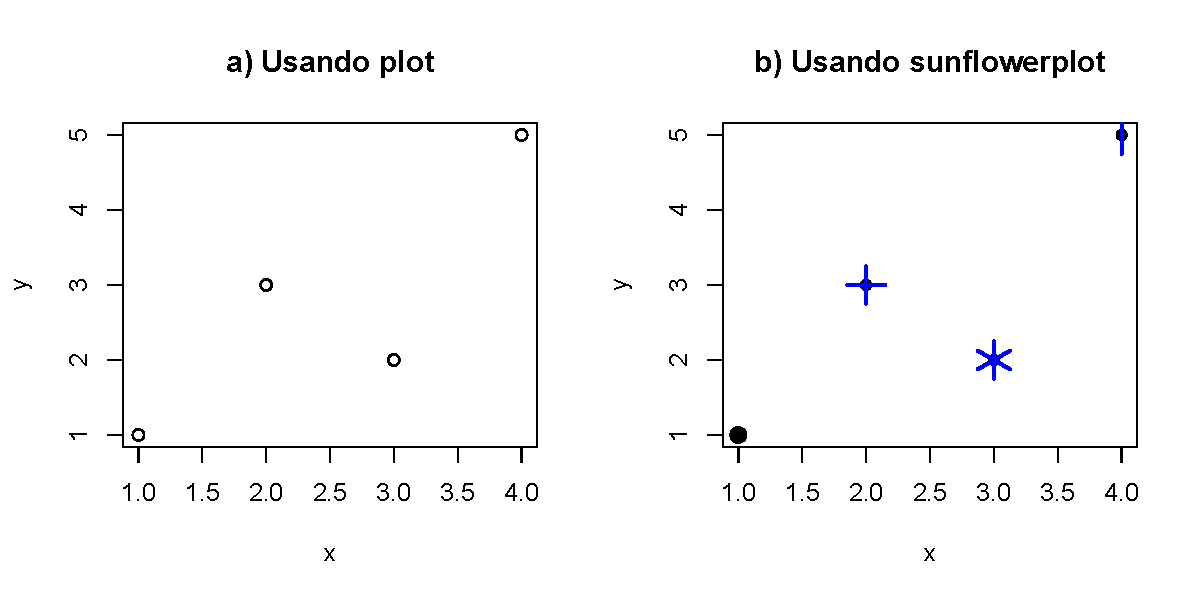
\includegraphics{Graficos_con_R_files/figure-latex/sunflower1-1.pdf}
\caption{\label{fig:sunflower1}Gráfico de dispersión para datos hipotéticos.
En la izquierda el gráfico obtenido con \texttt{plot} y a la derecha el
obtenido con \texttt{sunflowerplot}.}
\end{figure}

En la Figura \ref{fig:sunflower1} se muestran los dos gráficos de
dispersión para los datos. En el panel de la izquierda está el diagrama
obtenido con la función \texttt{plot} pero sólo se observan 4 puntos
cuando en realidad eran 13, esto se debe a que hay puntos repetidos y
éstos quedan unos sobre otros. En el panel de la derecha está el
diagrama obtenido con la función \texttt{sunflowerplot}, en este
diagrama se observan cuatro objetos: el punto con coordenadas (1, 1) se
representó con un punto ya que él no se repite, el punto (2, 3) está
representado por un punto y cuatro pétalos de color azul ya que él se
repite cuatro veces, y los puntos (3, 2) y (4, 5) se represetan con seis
y dos pétalos porque esas son las veces que ellos se repiten.

\subsection*{Ejemplo}\label{ejemplo-12}


Como ilustración vamos a crear un diagrama de dispersión con la función
\texttt{sunflowerplot} para las variables número de alcobas y número de
baños de la base de datos de apartamentos usados.

El código necesario para cargar la base de datos y construir el diagrama
de dispersión se muestra a continuación. El diagrama de dispersión se
construyó excluyendo la información del apartamento 594 porque éste
aparece con 14 alcobas.

\begin{Shaded}
\begin{Highlighting}[]
\NormalTok{url <-}\StringTok{ 'https://tinyurl.com/hwhb769'}
\NormalTok{datos <-}\StringTok{ }\KeywordTok{read.table}\NormalTok{(}\DataTypeTok{file=}\NormalTok{url, }\DataTypeTok{header=}\NormalTok{T)}
\NormalTok{datos <-}\StringTok{ }\NormalTok{datos[}\OperatorTok{-}\DecValTok{594}\NormalTok{, ]}
\KeywordTok{sunflowerplot}\NormalTok{(}\DataTypeTok{x=}\NormalTok{datos}\OperatorTok{$}\NormalTok{alcobas, }\DataTypeTok{y=}\NormalTok{datos}\OperatorTok{$}\NormalTok{banos)}
\end{Highlighting}
\end{Shaded}

\begin{figure}
\centering
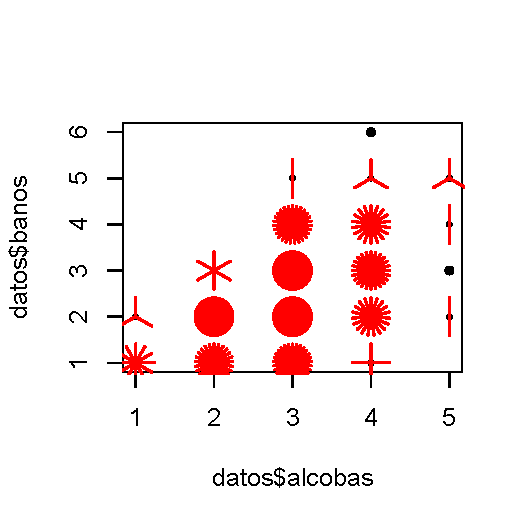
\includegraphics{Graficos_con_R_files/figure-latex/sunflower2-1.pdf}
\caption{\label{fig:sunflower2}Diagrama de dispersión para número de baños
versus número de alcobas.}
\end{figure}

En la Figura \ref{fig:sunflower2} se muestra el diagrama de dispersión
entre número de baños y número de alcobas. De este diagrama se observa
que la mayor parte de los apartamentos de la base de datos tienen 2 o 3
alcobas con 2 o 3 baños, se nota que sólo 8 apartamentos tiene 5 alcobas
y que sólo un apatamento tiene seis baños.

\section{\texorpdfstring{Función \texttt{symbols}
\index{symbols}}{Función symbols }}\label{funcion-symbols}

La función \texttt{symbols} sirve para construir diagramas de dispersión
en dos dimensiones incluyendo información adicional de variables
cuantitativas.

\subsection*{Ejemplo}\label{ejemplo-13}


Como ilustración vamos a crear un diagrama de dispersión entre el precio
de apartamentos usados en la ciudad de Medellín y el área de los
apartamentos pero incluyendo otras variables.

\begin{Shaded}
\begin{Highlighting}[]
\NormalTok{url <-}\StringTok{ 'https://tinyurl.com/hwhb769'}
\NormalTok{datos <-}\StringTok{ }\KeywordTok{read.table}\NormalTok{(url, }\DataTypeTok{header=}\NormalTok{T)}
\NormalTok{subdat <-}\StringTok{ }\KeywordTok{subset}\NormalTok{(datos, ubicacion }\OperatorTok{==}\StringTok{ 'centro'}\NormalTok{)}

\KeywordTok{par}\NormalTok{(}\DataTypeTok{mfrow=}\KeywordTok{c}\NormalTok{(}\DecValTok{1}\NormalTok{, }\DecValTok{2}\NormalTok{))}
\KeywordTok{with}\NormalTok{(subdat, }\KeywordTok{symbols}\NormalTok{(}\DataTypeTok{x=}\NormalTok{mt2, }\DataTypeTok{y=}\NormalTok{precio,}
                     \DataTypeTok{circles=}\NormalTok{alcobas, }
                     \DataTypeTok{las=}\DecValTok{1}\NormalTok{, }\DataTypeTok{inches=}\FloatTok{0.4}\NormalTok{, }
                     \DataTypeTok{fg=}\StringTok{'red'}\NormalTok{,}
                     \DataTypeTok{main=}\StringTok{'Radio = N° alcobas'}\NormalTok{))}

\KeywordTok{with}\NormalTok{(subdat, }\KeywordTok{symbols}\NormalTok{(}\DataTypeTok{x=}\NormalTok{mt2, }\DataTypeTok{y=}\NormalTok{precio,}
                     \DataTypeTok{squares=}\NormalTok{alcobas, }
                     \DataTypeTok{las=}\DecValTok{1}\NormalTok{, }\DataTypeTok{inches=}\FloatTok{0.4}\NormalTok{, }
                     \DataTypeTok{fg=}\StringTok{'dodgerblue4'}\NormalTok{, }\DataTypeTok{bg=}\StringTok{'pink'}\NormalTok{,}
                     \DataTypeTok{main=}\StringTok{'Lado = N° alcobas'}\NormalTok{))}
\end{Highlighting}
\end{Shaded}

\begin{figure}
\centering
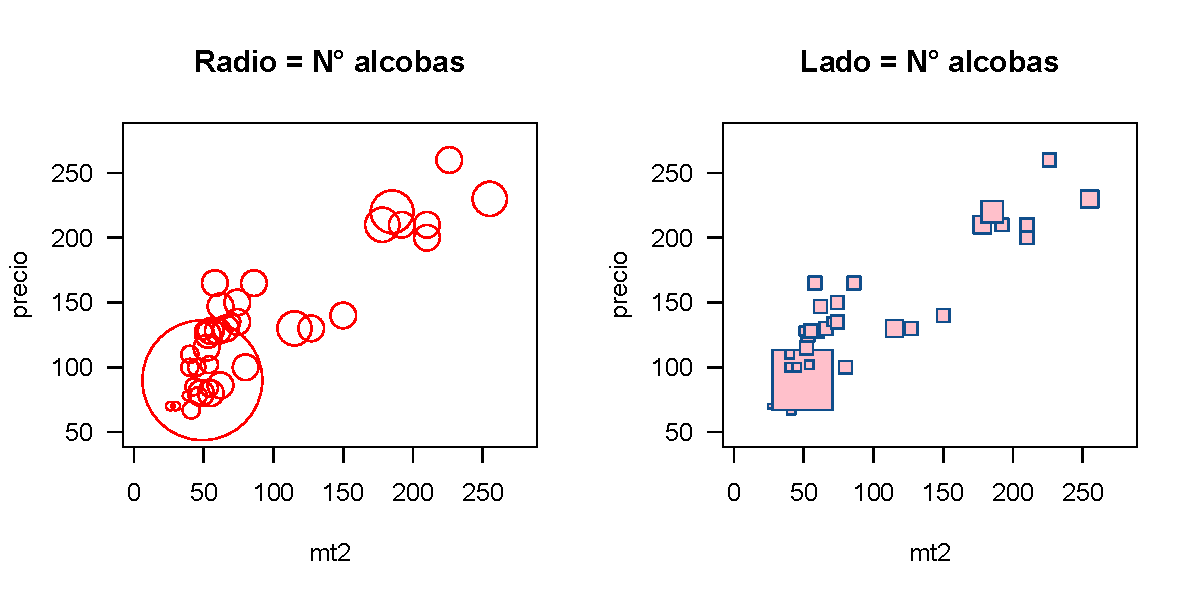
\includegraphics{Graficos_con_R_files/figure-latex/symbols1-1.pdf}
\caption{\label{fig:symbols1}Diagrama de dispersión con los símbolos circle
y squares para incluir más variables.}
\end{figure}

\begin{Shaded}
\begin{Highlighting}[]
\KeywordTok{par}\NormalTok{(}\DataTypeTok{mfrow=}\KeywordTok{c}\NormalTok{(}\DecValTok{1}\NormalTok{, }\DecValTok{2}\NormalTok{))}
\KeywordTok{with}\NormalTok{(subdat, }\KeywordTok{symbols}\NormalTok{(}\DataTypeTok{x=}\NormalTok{mt2, }\DataTypeTok{y=}\NormalTok{precio,}
                     \DataTypeTok{rectangles=}\KeywordTok{cbind}\NormalTok{(estrato, alcobas), }
                     \DataTypeTok{las=}\DecValTok{1}\NormalTok{, }\DataTypeTok{inches=}\FloatTok{0.4}\NormalTok{, }
                     \DataTypeTok{fg=}\StringTok{'chartreuse4'}\NormalTok{, }\DataTypeTok{bg=}\StringTok{'yellow'}\NormalTok{,}
                     \DataTypeTok{main=}\StringTok{'Ancho = estrato y Alto = N° alcobas'}\NormalTok{))}

\KeywordTok{with}\NormalTok{(subdat, }\KeywordTok{symbols}\NormalTok{(}\DataTypeTok{x=}\NormalTok{mt2, }\DataTypeTok{y=}\NormalTok{precio,}
                     \DataTypeTok{stars=}\KeywordTok{cbind}\NormalTok{(estrato, alcobas,}
\NormalTok{                                 banos), }
                     \DataTypeTok{las=}\DecValTok{1}\NormalTok{, }\DataTypeTok{inches=}\FloatTok{0.4}\NormalTok{, }
                     \DataTypeTok{fg=}\StringTok{'purple1'}\NormalTok{, }\DataTypeTok{bg=}\StringTok{'tomato'}\NormalTok{,}
                     \DataTypeTok{main=}\StringTok{'Estrato, alcobas y n° baños'}\NormalTok{))}
\end{Highlighting}
\end{Shaded}

\begin{figure}
\centering
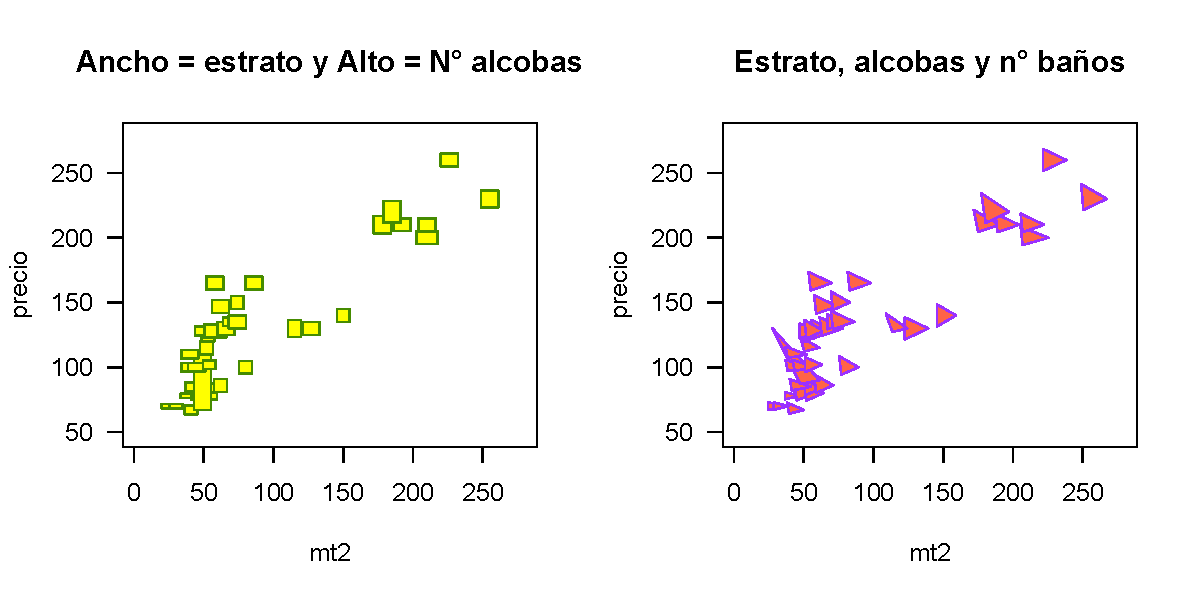
\includegraphics{Graficos_con_R_files/figure-latex/symbols2-1.pdf}
\caption{\label{fig:symbols2}Diagrama de dispersión con los símbolos
rectangles y stars para incluir más variables.}
\end{figure}

\section{\texorpdfstring{Función \texttt{pairs}
\index{pairs}}{Función pairs }}\label{funcion-pairs}

Las matrices de dispersión obtenidas con la función \texttt{pairs}
proporcionan un método simple de presentar las relaciones entre pares de
variables cuantitativas y son la versión múltiple de la función
\texttt{plot}. Este gráfico consiste en una matriz donde cada entrada
presenta un gráfico de dispersión sencillo. Un inconveniente es que si
tenemos muchas variables el tamaño de cada entrada se reduce demasiado
impidiendo ver con claridad las relaciones entre los pares de variables.
La celda \((i,j)\) de una matriz de dispersión contiene el gráfico de
dispersión de la columna \(i\) versus la columna \(j\) de la matriz de
datos.

En la Figura \ref{fig:ex0pairs} se muestra un ejemplo de una matriz de
dispersión para un conjunto de datos, en la diagonal están los nombres
de las variables y por fuera de la diagonal están los diagramas de
dispersión para cada combinación de variables.

\begin{figure}
\centering
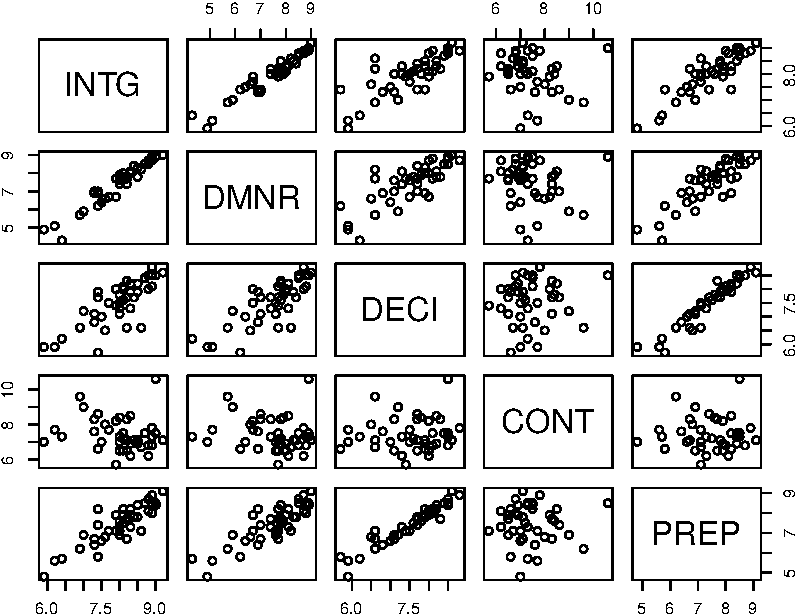
\includegraphics{Graficos_con_R_files/figure-latex/ex0pairs-1.pdf}
\caption{\label{fig:ex0pairs}Ilustración de una matriz de dispersión.}
\end{figure}

La estructura de la función \texttt{pairs} con los argumentos más
usuales se muestra a continuación:

\begin{Shaded}
\begin{Highlighting}[]
\KeywordTok{pairs}\NormalTok{(x, labels, }\DataTypeTok{panel =}\NormalTok{ points, ...,}
      \DataTypeTok{horInd =} \DecValTok{1}\OperatorTok{:}\NormalTok{nc, }\DataTypeTok{verInd =} \DecValTok{1}\OperatorTok{:}\NormalTok{nc,}
      \DataTypeTok{lower.panel =}\NormalTok{ panel, }\DataTypeTok{upper.panel =}\NormalTok{ panel,}
      \DataTypeTok{diag.panel =} \OtherTok{NULL}\NormalTok{, }\DataTypeTok{text.panel =}\NormalTok{ textPanel,}
      \DataTypeTok{label.pos =} \FloatTok{0.5} \OperatorTok{+}\StringTok{ }\NormalTok{has.diag}\OperatorTok{/}\DecValTok{3}\NormalTok{, }\DataTypeTok{line.main =} \DecValTok{3}\NormalTok{,}
      \DataTypeTok{cex.labels =} \OtherTok{NULL}\NormalTok{, }\DataTypeTok{font.labels =} \DecValTok{1}\NormalTok{,}
      \DataTypeTok{row1attop =} \OtherTok{TRUE}\NormalTok{, }\DataTypeTok{gap =} \DecValTok{1}\NormalTok{, }\DataTypeTok{log =} \StringTok{""}\NormalTok{)}
\end{Highlighting}
\end{Shaded}

Los argumentos de la función \texttt{pairs} son:

\begin{itemize}
\tightlist
\item
  \texttt{x}: matriz o marco de datos con la información de las
  variables cuantitativas a incluir en la matriz de dispersión.
\item
  \texttt{labels}: vector opcional con los nombres a colocar en la
  diagonal, por defecto se usan los nombres de columnas del objeto
  \texttt{x}.
\item
  \texttt{panel}: función usual de la forma \texttt{function(x,y,...)} a
  ser usada para determinar el contenido de los páneles. Por defecto es
  \texttt{points}, indicando que se graficarán los puntos de los pares
  de variables. Es posible utilizar aquí otras funciones diseñadas por
  el usuario.
\item
  \texttt{...}: Indica que es posible agregar otros parámetros gráficos,
  tales como \texttt{pch} y \texttt{col}, con los cuales puede
  especificarse un vector de símbolos y colores a ser usados en los
  scatterplots.
\item
  \texttt{lower.panel,\ upper.panel}: función usual de la forma
  \texttt{function(x,y,...)} para definir lo que se desea dibujar en los
  paneles abajo y arriba de la diagonal.
\item
  \texttt{diag.panel}: función usual de la forma
  \texttt{function(x,y,...)} para definir lo que se desea dibujar en la
  diagonal.
\item
  \texttt{text.panel}: Es opcional. Permite que una función:
  \texttt{function(x,\ y,\ labels,\ cex,\ font,\ ...)} sea aplicada a
  los paneles de la diagonal.
\item
  \texttt{label.pos}: Para especificar la posición \(y\) de las
  etiquetas en el text panel.
\item
  \texttt{cex.labels,\ font.labels}: Parámetros para la expansión de
  caracteres y fuentes a usar en las etiquetas de las variables.
\item
  \texttt{row1attop}: Parámetro lógico con el cual se especifica si el
  gráfico para especificar si el diseño lucirá como una matriz con su
  primera fila en la parte superior o como un gráfico con fila uno en la
  base. Por defecto es lo primero.
\end{itemize}

\subsection*{Ejemplo}\label{ejemplo-14}


Dibujar una matriz de dispersión para las variables precio, área, número
de alcobas y número de baños de la base de datos sobre apartamentos en
Medellín.

A continuación se muestra el código usado para crear el gráfico
solicitado. El objeto \texttt{datos} corresponde a la base de datos
completa mientras que \texttt{datos.num} es el marco de datos sólo con
las variables de interés precio, área, número de alcobas y número de
baños.

\begin{Shaded}
\begin{Highlighting}[]
\NormalTok{url <-}\StringTok{ 'https://raw.githubusercontent.com/fhernanb/datos/master/aptos2015'}
\NormalTok{datos <-}\StringTok{ }\KeywordTok{read.table}\NormalTok{(}\DataTypeTok{file=}\NormalTok{url, }\DataTypeTok{header=}\NormalTok{T)}
\NormalTok{datos.num <-}\StringTok{ }\NormalTok{datos[, }\KeywordTok{c}\NormalTok{(}\StringTok{'precio'}\NormalTok{, }\StringTok{'mt2'}\NormalTok{, }\StringTok{'alcobas'}\NormalTok{, }\StringTok{'banos'}\NormalTok{)]}

\KeywordTok{pairs}\NormalTok{(datos.num)}
\end{Highlighting}
\end{Shaded}

\begin{figure}
\centering
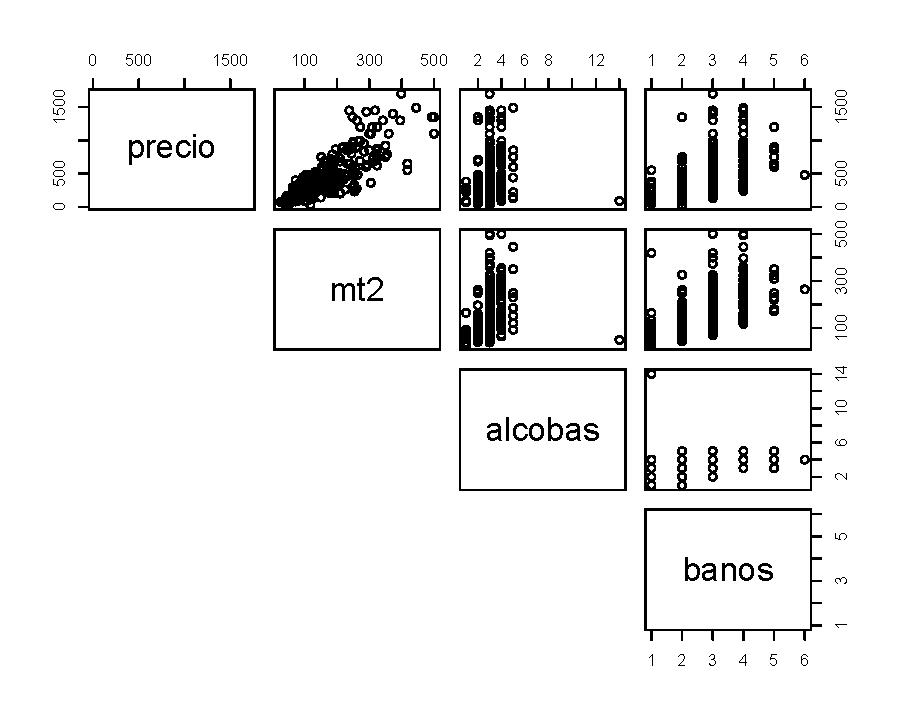
\includegraphics{Graficos_con_R_files/figure-latex/ex1pairs-1.pdf}
\caption{\label{fig:ex1pairs}Matriz de dispersión para las variables precio,
área, número de alcobas y número de baños de la base de datos sobre
apartamentos en Medellín.}
\end{figure}

En la Figura \ref{fig:ex1pairs} se muestra la matriz de dispersión para
las variables del marco de datos \texttt{datos.num}.

\subsection*{Ejemplo}\label{ejemplo-15}


Volver a construir la Figura \ref{fig:ex1pairs} editando los nombres de
las variables, usando cruces rojas en lugar de puntos, en escala
logaritmica, con marcas horizontales en el eje vertical y eliminando los
diagramas de dispersión abajo de la diagonal.

Para obtener la nueva matriz de dispersión con los cambios solicitados
se usa el siguiente código. En la Figura \ref{fig:ex2pairs} se presenta
la nueva matriz de dispersión.

\begin{Shaded}
\begin{Highlighting}[]
\KeywordTok{pairs}\NormalTok{(datos.num, }\DataTypeTok{lower.panel=}\OtherTok{NULL}\NormalTok{, }\DataTypeTok{cex.labels=}\FloatTok{1.5}\NormalTok{, }\DataTypeTok{log=}\StringTok{'xy'}\NormalTok{,}
      \DataTypeTok{main=}\StringTok{'Matriz de dispersión', las=1,}
\StringTok{      labels=c('}\NormalTok{Precio}\StringTok{', '}\NormalTok{Área}\StringTok{', '}\NormalTok{Num alcobas}\StringTok{', '}\NormalTok{Num baños}\StringTok{'),}
\StringTok{      pch=3, cex=0.6, col='}\NormalTok{red}\StringTok{')}
\end{Highlighting}
\end{Shaded}

\begin{figure}
\centering
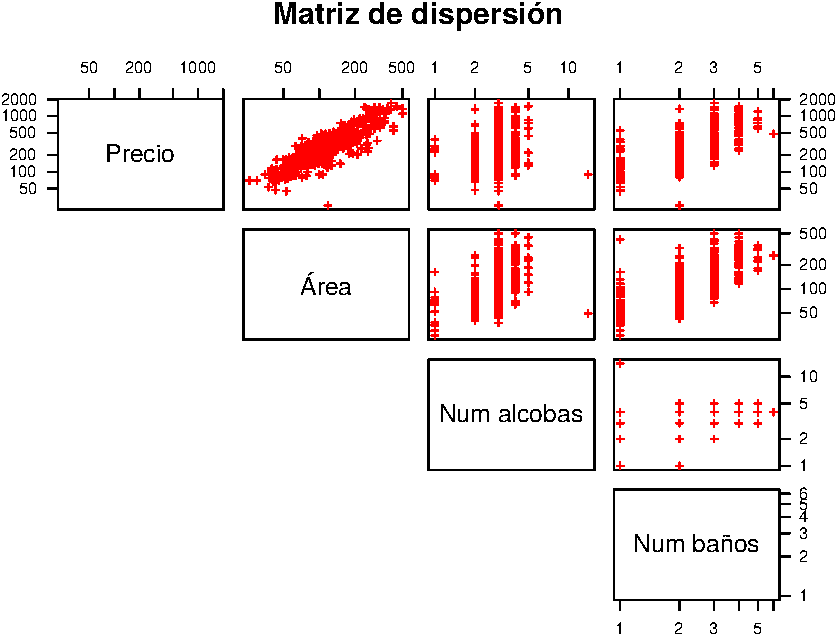
\includegraphics{Graficos_con_R_files/figure-latex/ex2pairs-1.pdf}
\caption{\label{fig:ex2pairs}Matriz de dispersión modificando los parámetros
adicionales de la función pairs.}
\end{figure}

\subsection*{Ejemplo}\label{ejemplo-16}


Construir una matriz de dispersión con las variables precio, área y
avaluo para apartamentos que cumplan la condición
\(100 m^2 < area < 130 m^2\). Adicionalmente, se deben diferenciar los
apartamentos sin parqueadero con color rojo y los apartamentos con
parqueadero con color verde.

Para crear una matriz de dispersión se puede tambien usar la base de
datos original llamada \texttt{datos} que contiene todas las variables y
usar una fórmula con la ayuda del operador \texttt{\textasciitilde{}}
para indicar las variables de interés. La fórmula \textbf{NO} debe
contener nada del lado izquierdo mientras que en el lado derecho se
colocan todas las variables a considerar en la matriz de dispersión, por
esta razón es que en el códido mostrado abajo se inicia con la
instrucción \texttt{\textasciitilde{}\ precio\ +\ mt2\ +\ avaluo}. Para
incluir condiciones se usa el parámetro \texttt{subset} de la siguiente
manera:
\texttt{subset=mt2\ \textgreater{}\ 100\ \&\ mt2\ \textless{}\ 130}. A
continuación el código completo para construir la matriz de dispersión
solicitada.

\begin{Shaded}
\begin{Highlighting}[]
\NormalTok{col1 <-}\StringTok{ }\KeywordTok{ifelse}\NormalTok{(datos}\OperatorTok{$}\NormalTok{parqueadero }\OperatorTok{==}\StringTok{ 'no'}\NormalTok{, }\StringTok{'red'}\NormalTok{, }\StringTok{'green3'}\NormalTok{)}
\KeywordTok{pairs}\NormalTok{(}\OperatorTok{~}\StringTok{ }\NormalTok{precio }\OperatorTok{+}\StringTok{ }\NormalTok{mt2 }\OperatorTok{+}\StringTok{ }\NormalTok{avaluo, }\DataTypeTok{data=}\NormalTok{datos,}
      \DataTypeTok{lower.panel=}\OtherTok{NULL}\NormalTok{, }\DataTypeTok{col=}\NormalTok{col1,}
      \DataTypeTok{subset=}\NormalTok{mt2 }\OperatorTok{>}\StringTok{ }\DecValTok{100} \OperatorTok{&}\StringTok{ }\NormalTok{mt2 }\OperatorTok{<}\StringTok{ }\DecValTok{130}\NormalTok{, }\DataTypeTok{pch=}\DecValTok{19}\NormalTok{, }\DataTypeTok{cex=}\FloatTok{0.8}\NormalTok{,}
      \DataTypeTok{main=}\StringTok{"Matriz de dispersión para aptos con }
\StringTok{      100 < área < 130 mt2"}\NormalTok{)}
\end{Highlighting}
\end{Shaded}

\begin{figure}
\centering
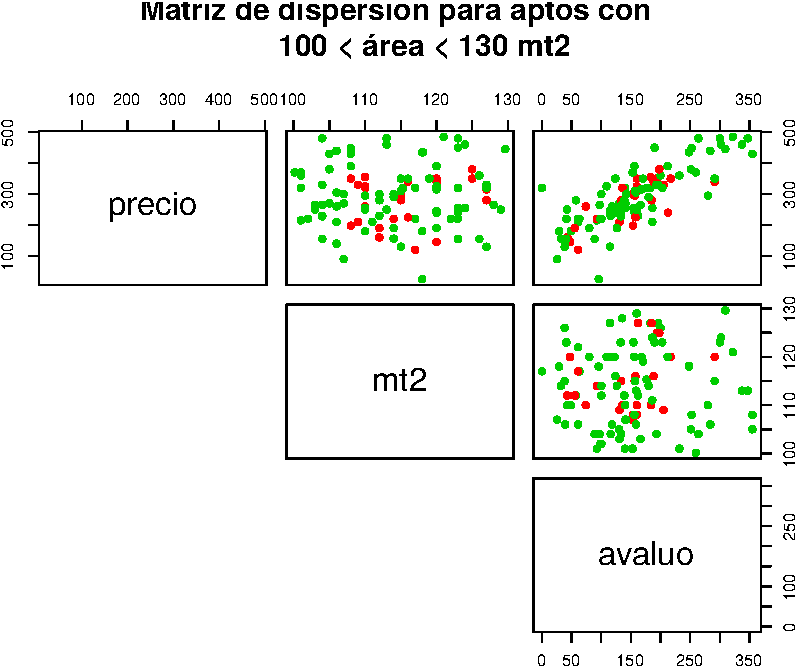
\includegraphics{Graficos_con_R_files/figure-latex/ex3pairs-1.pdf}
\caption{\label{fig:ex3pairs}Matriz de dispersión con un subconjunto de los
datos y con colores para identificar los puntos.}
\end{figure}

En la Figura \ref{fig:ex3pairs} se presenta la matriz de dispersión
solicitada, los puntos rojos representan los apartamento sin parqueadero
mientras que los puntos verdes son los apartamento que si tienen
parqueadero.

\subsection*{Ejemplo}\label{ejemplo-17}


¿Es posible agregar una leyenda a una matriz de dispersión?

Claro que es posible, se construye la matriz de dispersión y se deja en
el lienzo del dibujo un espacio para colocar la leyenda. A continuación
se muestra un ejemplo disponible en
\href{http://stackoverflow.com/questions/14948852/how-to-use-the-pairs-function-combined-with-layout-in-r}{Stackoverflow}.
A continuación se muestra el código para el ejemplo y en la Figura
\ref{fig:expairs} se presenta el resultado.

\begin{Shaded}
\begin{Highlighting}[]
\KeywordTok{pairs}\NormalTok{(iris[}\DecValTok{1}\OperatorTok{:}\DecValTok{4}\NormalTok{], }\DataTypeTok{main=}\StringTok{"Anderson's Iris Data -- 3 species"}\NormalTok{,}
      \DataTypeTok{pch=}\DecValTok{21}\NormalTok{, }\DataTypeTok{bg=}\KeywordTok{c}\NormalTok{(}\StringTok{"red"}\NormalTok{, }\StringTok{"green3"}\NormalTok{, }\StringTok{"blue"}\NormalTok{)[iris}\OperatorTok{$}\NormalTok{Species],}
      \DataTypeTok{oma=}\KeywordTok{c}\NormalTok{(}\DecValTok{4}\NormalTok{, }\DecValTok{4}\NormalTok{, }\DecValTok{6}\NormalTok{, }\DecValTok{12}\NormalTok{))}
\KeywordTok{par}\NormalTok{(}\DataTypeTok{xpd=}\OtherTok{TRUE}\NormalTok{)}
\KeywordTok{legend}\NormalTok{(}\FloatTok{0.85}\NormalTok{, }\FloatTok{0.7}\NormalTok{, }\KeywordTok{as.vector}\NormalTok{(}\KeywordTok{unique}\NormalTok{(iris}\OperatorTok{$}\NormalTok{Species)), }\DataTypeTok{bty=}\StringTok{'n'}\NormalTok{,}
       \DataTypeTok{fill=}\KeywordTok{c}\NormalTok{(}\StringTok{"red"}\NormalTok{, }\StringTok{"green3"}\NormalTok{, }\StringTok{"blue"}\NormalTok{))}
\end{Highlighting}
\end{Shaded}

\begin{figure}
\centering
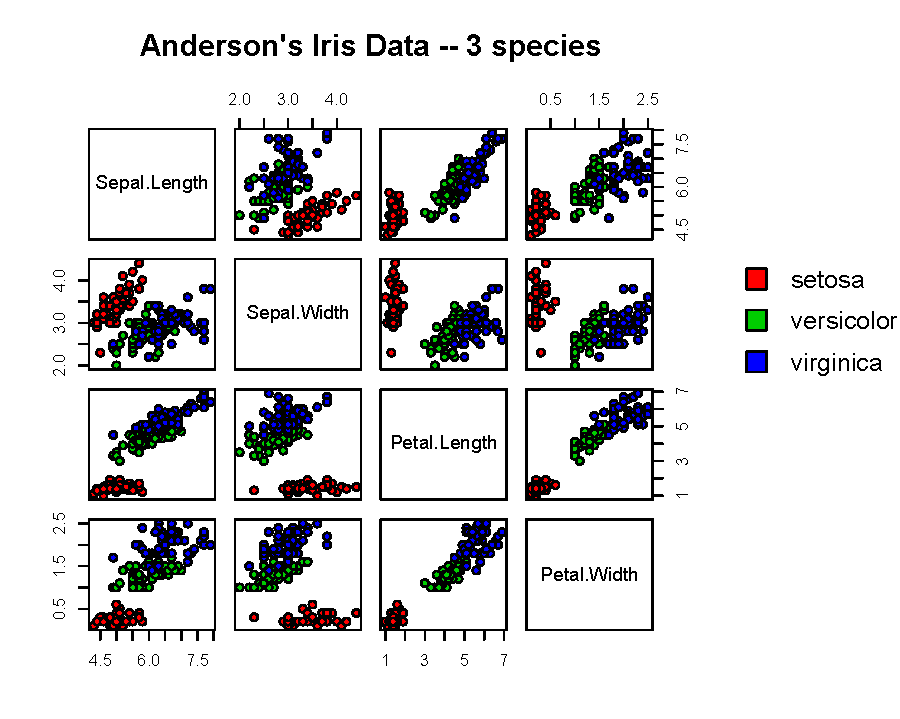
\includegraphics{Graficos_con_R_files/figure-latex/expairs-1.pdf}
\caption{\label{fig:expairs}Matriz de dispersión con leyenda.}
\end{figure}

\subsection*{Ejemplo}\label{ejemplo-18}


¿Es posible modificar el contenido de los páneles de una matriz de
dispersión?

Claro que es posible, para hacer esto se definen funciones que hagan lo
que se desea ver tanto en la diagonal como arriba y abajo de la misma.

Como ejemplo vamos a construir una matriz de dispersión que cumpla:

\begin{itemize}
\tightlist
\item
  sobre la diagonal un diagrama de dispersión para las variables
  involucradas y la recta de regresión ajustada,
\item
  en la diagonal un histograma para la variable,
\item
  debajo de la diagonal el coeficiente de correlación entre las
  variables involucradas y usando un tamaño de fuente proporcional a la
  fuerza de correlación.
\end{itemize}

Para obtener esta matriz de dispersión especial se definen a
continuación las funciones \texttt{panel.reg}, \texttt{panel.hist} y
\texttt{panel.cor}, a continuación el código utilizado. Luego se usa la
función \texttt{pairs} y se indica qué función debe actuar en cada uno
de los parámetros \texttt{upper.panel}, \texttt{diag.panel} y
\texttt{lower.panel}.

\begin{Shaded}
\begin{Highlighting}[]
\CommentTok{# Función para dibujar los puntos y agregar la recta de regresión}
\NormalTok{panel.reg <-}\StringTok{ }\ControlFlowTok{function}\NormalTok{ (x, y) }
\NormalTok{\{}
  \KeywordTok{points}\NormalTok{(x, y, }\DataTypeTok{pch=}\DecValTok{20}\NormalTok{)}
  \KeywordTok{abline}\NormalTok{(}\KeywordTok{lm}\NormalTok{(y }\OperatorTok{~}\StringTok{ }\NormalTok{x), }\DataTypeTok{lwd=}\DecValTok{2}\NormalTok{, }\DataTypeTok{col=}\StringTok{'dodgerblue2'}\NormalTok{)}
\NormalTok{\}}

\CommentTok{# Función para crear el histograma}
\NormalTok{panel.hist <-}\StringTok{ }\ControlFlowTok{function}\NormalTok{(x, ...)}
\NormalTok{\{}
\NormalTok{  usr <-}\StringTok{ }\KeywordTok{par}\NormalTok{(}\StringTok{"usr"}\NormalTok{); }\KeywordTok{on.exit}\NormalTok{(}\KeywordTok{par}\NormalTok{(usr))}
  \KeywordTok{par}\NormalTok{(}\DataTypeTok{usr =} \KeywordTok{c}\NormalTok{(usr[}\DecValTok{1}\OperatorTok{:}\DecValTok{2}\NormalTok{], }\DecValTok{0}\NormalTok{, }\FloatTok{1.5}\NormalTok{) )}
\NormalTok{  h <-}\StringTok{ }\KeywordTok{hist}\NormalTok{(x, }\DataTypeTok{plot =} \OtherTok{FALSE}\NormalTok{)}
\NormalTok{  breaks <-}\StringTok{ }\NormalTok{h}\OperatorTok{$}\NormalTok{breaks; nB <-}\StringTok{ }\KeywordTok{length}\NormalTok{(breaks)}
\NormalTok{  y <-}\StringTok{ }\NormalTok{h}\OperatorTok{$}\NormalTok{counts; y <-}\StringTok{ }\NormalTok{y}\OperatorTok{/}\KeywordTok{max}\NormalTok{(y)}
  \KeywordTok{rect}\NormalTok{(breaks[}\OperatorTok{-}\NormalTok{nB], }\DecValTok{0}\NormalTok{, breaks[}\OperatorTok{-}\DecValTok{1}\NormalTok{], y, }\DataTypeTok{col=}\StringTok{"dodgerblue2"}\NormalTok{, ...)}
\NormalTok{\}}

\CommentTok{# Función para obtener la correlación}
\NormalTok{panel.cor <-}\StringTok{ }\ControlFlowTok{function}\NormalTok{(x, y, }\DataTypeTok{digits=}\DecValTok{2}\NormalTok{, }\DataTypeTok{prefix=}\StringTok{""}\NormalTok{, cex.cor)}
\NormalTok{\{}
\NormalTok{  usr <-}\StringTok{ }\KeywordTok{par}\NormalTok{(}\StringTok{"usr"}\NormalTok{); }\KeywordTok{on.exit}\NormalTok{(}\KeywordTok{par}\NormalTok{(usr))}
  \KeywordTok{par}\NormalTok{(}\DataTypeTok{usr =} \KeywordTok{c}\NormalTok{(}\DecValTok{0}\NormalTok{, }\DecValTok{1}\NormalTok{, }\DecValTok{0}\NormalTok{, }\DecValTok{1}\NormalTok{))}
\NormalTok{  r <-}\StringTok{ }\KeywordTok{abs}\NormalTok{(}\KeywordTok{cor}\NormalTok{(x, y))}
\NormalTok{  txt <-}\StringTok{ }\KeywordTok{format}\NormalTok{(}\KeywordTok{c}\NormalTok{(r, }\FloatTok{0.123456789}\NormalTok{), }\DataTypeTok{digits=}\NormalTok{digits)[}\DecValTok{1}\NormalTok{]}
\NormalTok{  txt <-}\StringTok{ }\KeywordTok{paste}\NormalTok{(prefix, txt, }\DataTypeTok{sep=}\StringTok{""}\NormalTok{)}
  \ControlFlowTok{if}\NormalTok{(}\KeywordTok{missing}\NormalTok{(cex.cor)) cex <-}\StringTok{ }\FloatTok{0.8}\OperatorTok{/}\KeywordTok{strwidth}\NormalTok{(txt)}
  \KeywordTok{text}\NormalTok{(}\FloatTok{0.5}\NormalTok{, }\FloatTok{0.5}\NormalTok{, txt, }\DataTypeTok{cex =}\NormalTok{ cex }\OperatorTok{*}\StringTok{ }\NormalTok{r)}
\NormalTok{\}}

\KeywordTok{pairs}\NormalTok{(datos.num,}
      \DataTypeTok{upper.panel =}\NormalTok{ panel.reg,}
      \DataTypeTok{diag.panel =}\NormalTok{ panel.hist,}
      \DataTypeTok{lower.panel =}\NormalTok{ panel.cor)}
\end{Highlighting}
\end{Shaded}

\begin{figure}
\centering
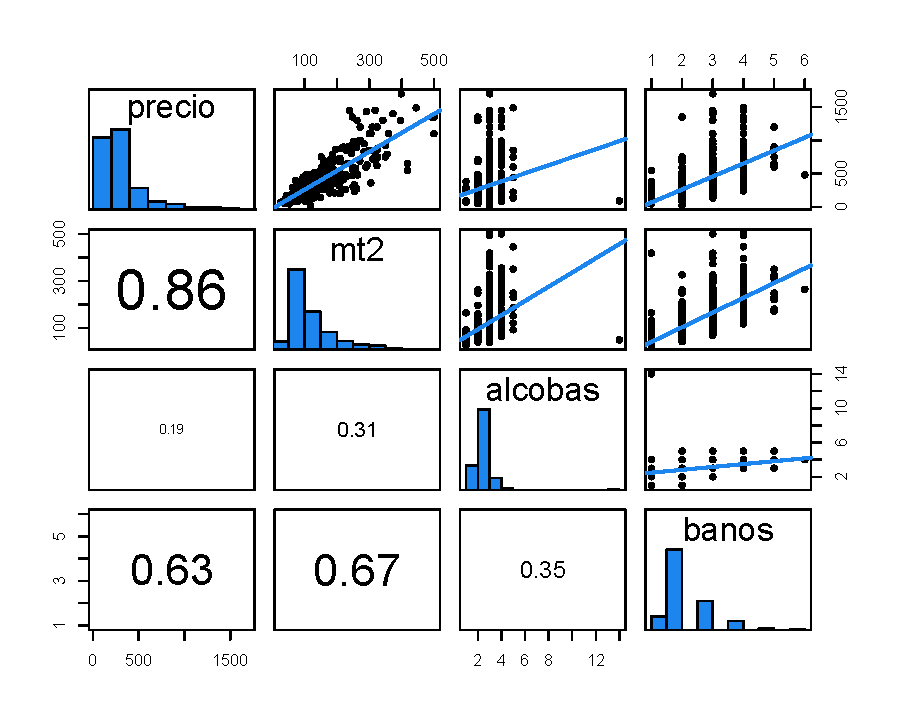
\includegraphics{Graficos_con_R_files/figure-latex/exmod1pairs-1.pdf}
\caption{\label{fig:exmod1pairs}Matriz de dispersión con páneles
modificados.}
\end{figure}

En la Figura \ref{fig:exmod1pairs} se presenta la matriz de dispersión
con las modificaciones en cada uno de los páneles. Cualquier usuario
puede modificar las funciones \texttt{panel.reg}, \texttt{panel.hist} y
\texttt{panel.cor} para personalizar la apariencia de los contenidos.

La función \texttt{panel.smooth} está disponible en \proglang{R} para
que el usuario pueda incluir arriba o abajo de la diagonal un diagrama
de dispersión con una línea resultado de un ajuste suavizado. Abajo se
muestra el código de cómo incluir la función \texttt{panel.smooth} y en
la Figura \ref{fig:exmod2pairs} se muestra gráfico obtenido.

\begin{Shaded}
\begin{Highlighting}[]
\KeywordTok{pairs}\NormalTok{(datos.num,}
      \DataTypeTok{upper.panel =}\NormalTok{ panel.reg,}
      \DataTypeTok{diag.panel =}\NormalTok{ panel.hist,}
      \DataTypeTok{lower.panel =}\NormalTok{ panel.smooth)}
\end{Highlighting}
\end{Shaded}

\begin{figure}
\centering
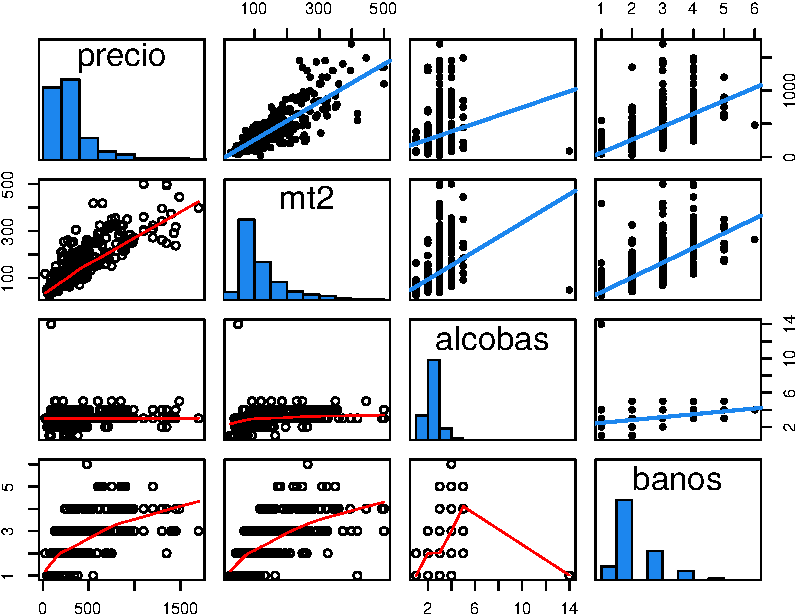
\includegraphics{Graficos_con_R_files/figure-latex/exmod2pairs-1.pdf}
\caption{\label{fig:exmod2pairs}Matriz de dispersión usando la función
panel.smooth.}
\end{figure}

\section{\texorpdfstring{Función \texttt{persp}
\index{persp}}{Función persp }}\label{funcion-persp}

La función \texttt{persp} dibuja superfices en tres dimensiones y es
posible rotar la superficie para obtener una perpectiva apropiada. La
estructura de la función \texttt{persp} con los argumentos más usuales
se muestra a continuación:

\begin{Shaded}
\begin{Highlighting}[]
\KeywordTok{persp}\NormalTok{(x, y, z, main, sub, theta, phi, r, col,}
\NormalTok{      border, box, axes, nticks)}
\end{Highlighting}
\end{Shaded}

Los argumentos de la función \texttt{plot} son:

\begin{itemize}
\tightlist
\item
  \texttt{x}: vector numérico con los valores de \(x\) donde fue
  evaluada la función o superficie.
\item
  \texttt{y}: vector numérico con los valores de \(y\) donde fue
  evaluada la función o superficie.
\item
  \texttt{z}: matriz que contiene las alturas \(z\) de la supercifie
  para cada combinación de \(x\) e \(y\).
\item
  \texttt{main}: vector numérico con las coordenadas del eje vertical.
\item
  \texttt{sub}: vector numérico con las coordenadas del eje vertical.
\item
  \texttt{theta,\ phi}: ángulo para la visión de la superficie,
  \texttt{theta} para la dirección azimutal y \texttt{phi} para latitud.
  Ver Figura \ref{fig:globo} para una ilustración de los ángulos.
\item
  \texttt{r}: distancia entre el centro de la caja de dibujo al punto de
  vista.
\item
  \texttt{col}: color de la superficie.
\item
  \texttt{border}: color para el borde de la superficie.
\item
  \texttt{box}: valor lógico para indicar si se quiere dibujar la caja
  que contiene la superficie, por defecto es \texttt{TRUE}.
\item
  \texttt{axes}: valor lógico para indicar si se desean marcas en los
  ejes y nombres de los ejes, por defecto es \texttt{TRUE}. Si
  \texttt{box=\textquotesingle{}FALSE\textquotesingle{}} no aparecen
  marcas ni nombres de los ejes.
\item
  \texttt{expand}: factor de expansión aplicado a los valores en el eje
  \texttt{z}.
\item
  \texttt{ticktype}: tipo de marcas a colocar en los ejes,
  \texttt{simple} no dibuja nada y \texttt{detailed} coloca números a
  los ejes.
\item
  \texttt{nticks}: número aproximado de marcas en los ejes.
\end{itemize}

\begin{figure}

{\centering 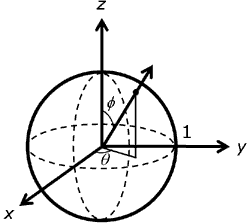
\includegraphics[width=0.4\linewidth]{images/IC412528} 

}

\caption{Ilustración de los ángulos theta y phi para la función persp. Figura tomada de https://i-msdn.sec.s-msft.com/dynimg/IC412528.png}\label{fig:globo}
\end{figure}

\subsection*{Ejemplo}\label{ejemplo-19}


Dibujar la superficie asociada a la función \(f(x, y)=sen(x^2+y^2)\)
para \(-2 \leq x \leq2\) y \(-2 \leq y \leq2\). Usar 4 combinaciones de
los parámetros \texttt{theta} y \texttt{phi} para obtener un buen punto
de vista de la superficie.

Lo primero que se debe hacer es crear la función \(f(x, y)\) la cual se
va a llamar \texttt{fun}. Luego se definen los vectores \texttt{x} e
\texttt{y} tomando por ejemplo 25 puntos equiespaciados en el intervalo
\([-2, 2]\). Luego se usa la función \texttt{outer} para crear la
rejilla o matriz que contiene los valores de \(f(x, y)\) para cada
combinación de \texttt{x} e \texttt{y}, los resultados se almacenan en
el objeto \texttt{z}. Por último se dibujan 4 perspectivas de la función
variando los parámetros \texttt{theta} y \texttt{phi} de la función
\texttt{persp}. A continuación el código utilizado.

\begin{Shaded}
\begin{Highlighting}[]
\NormalTok{fun <-}\StringTok{ }\ControlFlowTok{function}\NormalTok{(x, y)   }\KeywordTok{sin}\NormalTok{(x}\OperatorTok{^}\DecValTok{2} \OperatorTok{+}\StringTok{ }\NormalTok{y}\OperatorTok{^}\DecValTok{2}\NormalTok{)}
\NormalTok{x <-}\StringTok{ }\KeywordTok{seq}\NormalTok{(}\DataTypeTok{from=}\OperatorTok{-}\DecValTok{2}\NormalTok{, }\DataTypeTok{to=}\DecValTok{2}\NormalTok{, }\DataTypeTok{length.out=}\DecValTok{25}\NormalTok{)}
\NormalTok{y <-}\StringTok{ }\KeywordTok{seq}\NormalTok{(}\DataTypeTok{from=}\OperatorTok{-}\DecValTok{2}\NormalTok{, }\DataTypeTok{to=}\DecValTok{2}\NormalTok{, }\DataTypeTok{length.out=}\DecValTok{25}\NormalTok{)}
\NormalTok{z <-}\StringTok{ }\KeywordTok{outer}\NormalTok{(x, y, fun)}

\KeywordTok{par}\NormalTok{(}\DataTypeTok{mfrow=}\KeywordTok{c}\NormalTok{(}\DecValTok{2}\NormalTok{, }\DecValTok{2}\NormalTok{), }\DataTypeTok{mar=}\KeywordTok{c}\NormalTok{(}\DecValTok{1}\NormalTok{, }\DecValTok{1}\NormalTok{, }\DecValTok{2}\NormalTok{, }\DecValTok{1}\NormalTok{))}
\KeywordTok{persp}\NormalTok{(x, y, z, }\DataTypeTok{zlim=}\KeywordTok{c}\NormalTok{(}\OperatorTok{-}\DecValTok{1}\NormalTok{, }\FloatTok{1.5}\NormalTok{), }\DataTypeTok{theta=}\DecValTok{0}\NormalTok{, }\DataTypeTok{phi=}\DecValTok{0}\NormalTok{, }\DataTypeTok{col=}\StringTok{'aquamarine'}\NormalTok{,}
      \DataTypeTok{main=}\StringTok{'(A) theta=0, phi=0'}\NormalTok{)}
\KeywordTok{persp}\NormalTok{(x, y, z, }\DataTypeTok{zlim=}\KeywordTok{c}\NormalTok{(}\OperatorTok{-}\DecValTok{1}\NormalTok{, }\FloatTok{1.5}\NormalTok{), }\DataTypeTok{theta=}\DecValTok{15}\NormalTok{, }\DataTypeTok{phi=}\DecValTok{15}\NormalTok{, }\DataTypeTok{col=}\StringTok{'lightpink'}\NormalTok{,}
      \DataTypeTok{main=}\StringTok{'(B) theta=15, phi=15'}\NormalTok{)}
\KeywordTok{persp}\NormalTok{(x, y, z, }\DataTypeTok{zlim=}\KeywordTok{c}\NormalTok{(}\OperatorTok{-}\DecValTok{1}\NormalTok{, }\FloatTok{1.5}\NormalTok{), }\DataTypeTok{theta=}\DecValTok{45}\NormalTok{, }\DataTypeTok{phi=}\DecValTok{30}\NormalTok{, }\DataTypeTok{col=}\StringTok{'yellow1'}\NormalTok{,}
      \DataTypeTok{main=}\StringTok{'(c) theta=45, phi=30'}\NormalTok{)}
\KeywordTok{persp}\NormalTok{(x, y, z, }\DataTypeTok{zlim=}\KeywordTok{c}\NormalTok{(}\OperatorTok{-}\DecValTok{1}\NormalTok{, }\FloatTok{1.5}\NormalTok{), }\DataTypeTok{theta=}\DecValTok{60}\NormalTok{, }\DataTypeTok{phi=}\DecValTok{50}\NormalTok{, }\DataTypeTok{col=}\StringTok{'lightblue'}\NormalTok{,}
      \DataTypeTok{main=}\StringTok{'(D) theta=60, phi=50'}\NormalTok{)}
\end{Highlighting}
\end{Shaded}

\begin{figure}
\centering
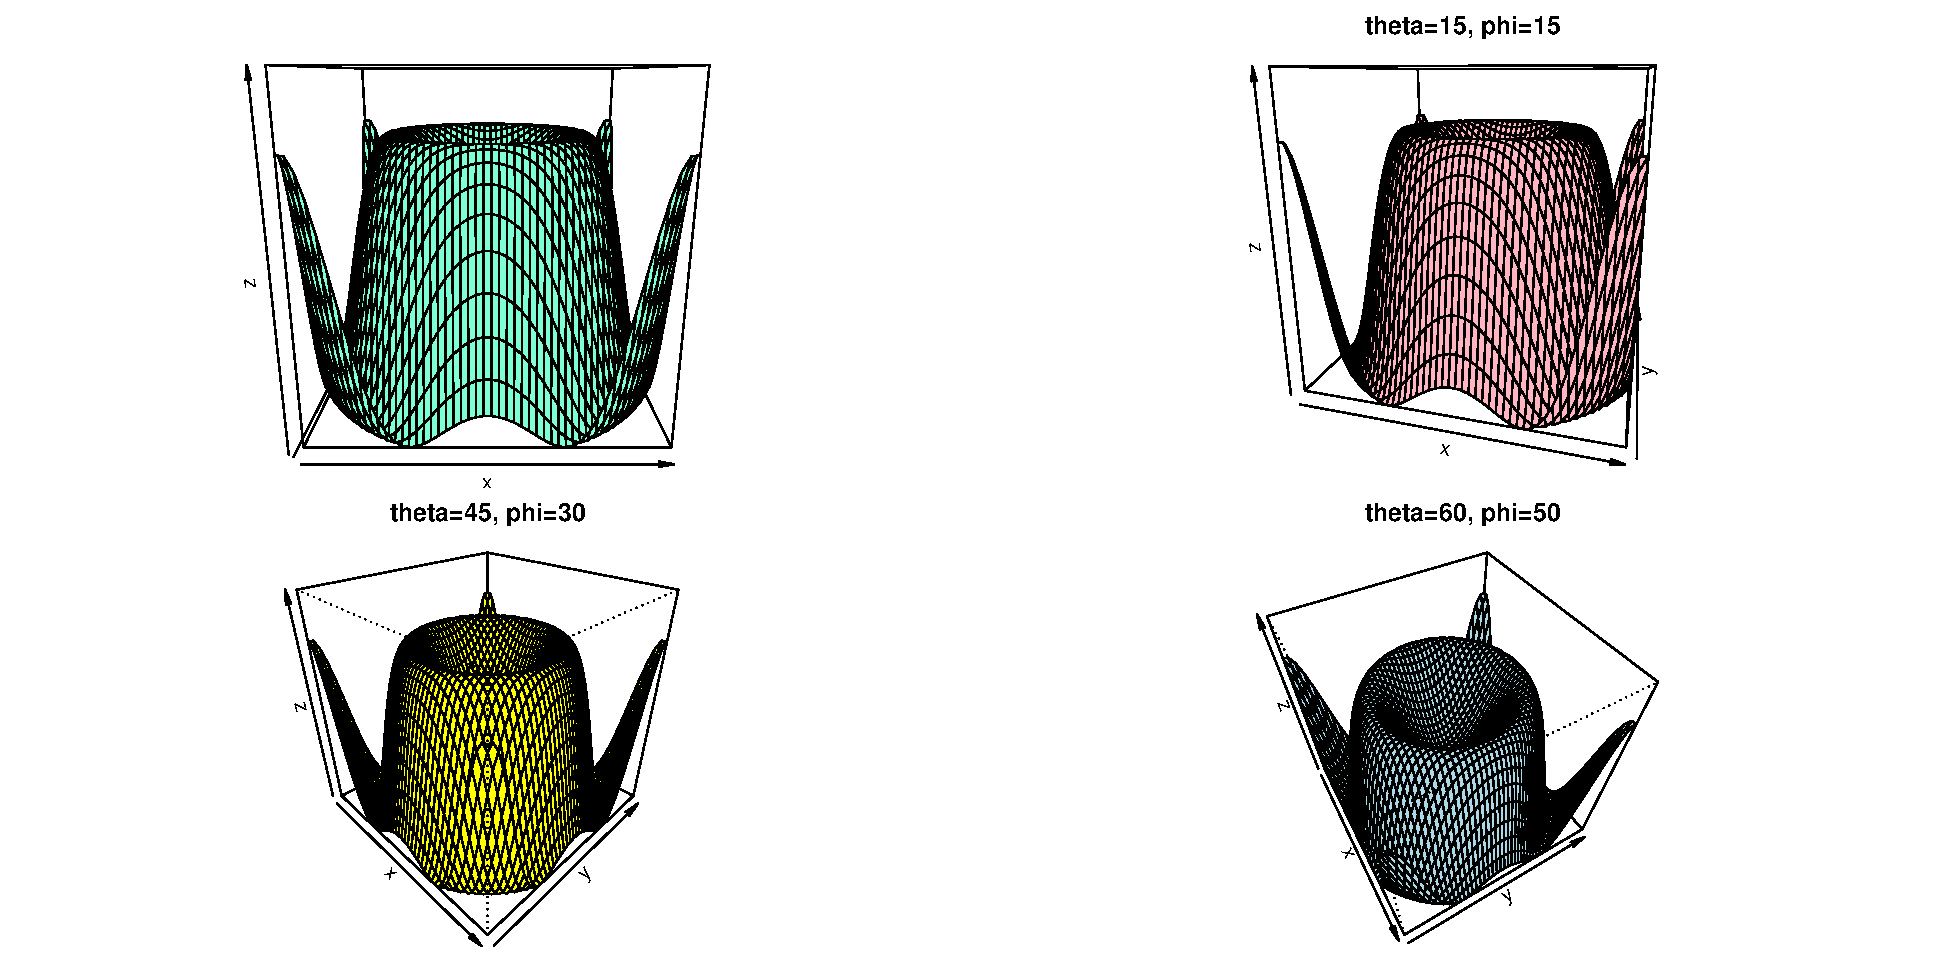
\includegraphics{Graficos_con_R_files/figure-latex/ex1persp-1.pdf}
\caption{\label{fig:ex1persp}Superficie generada con \texttt{persp} y
diferentes valores de theta y phi.}
\end{figure}

En la Figura \ref{fig:ex1persp} se presentan las 4 perspectivas de la
función \(f(x, y)=sen(x^2+y^2)\). De los 4 páneles se nota que (C) y (D)
muestran mejor la superficie de interés.

Al aumentar el valor del parámetro \texttt{length.out} en la creación de
los vectores \texttt{x} e \texttt{y} se obtendrá una rejilla más tupida,
se recomienda modificar este valor para obtener una superficie
apropiada.

\subsection*{Ejemplo}\label{ejemplo-20}


Dibujar la superficie de una distribución normal bivariada con vector de
medias \(\boldsymbol{\mu}=(5, 12)^\top\), varianzas unitarias y
covarianza con valor de -0.8. Explorar el efecto de los parámetros
\texttt{ticktype}, \texttt{nticks}, \texttt{expand}, \texttt{axes} y
\texttt{box}.

Primero se define el vector de medias y la matriz de varianzas y
covarianzas, luego se carga el paquete \texttt{mvtnorm} que contiene la
función \texttt{dmvnorm} que calcula la densidad dado el vector de
medias y la matriz de varianzas y covarianzas. Se construye la función
\texttt{fun} y se vectoriza para luego obtener las alturas de la
superficie con la ayuda de \texttt{outer}. Por último se dibujan tres
perspectivas diferentes para la densidad modificando los parámetros
\texttt{ticktype}, \texttt{nticks}, \texttt{expand}, \texttt{axes} y
\texttt{box}, a continuación el código usado.

\begin{Shaded}
\begin{Highlighting}[]
\NormalTok{media <-}\StringTok{ }\KeywordTok{c}\NormalTok{(}\DecValTok{5}\NormalTok{, }\DecValTok{12}\NormalTok{)}
\NormalTok{varianza <-}\StringTok{ }\KeywordTok{matrix}\NormalTok{(}\KeywordTok{c}\NormalTok{(}\DecValTok{1}\NormalTok{, }\OperatorTok{-}\FloatTok{0.8}\NormalTok{, }\OperatorTok{-}\FloatTok{0.8}\NormalTok{, }\DecValTok{1}\NormalTok{), }\DataTypeTok{ncol=}\DecValTok{2}\NormalTok{)}

\KeywordTok{require}\NormalTok{(mvtnorm)}
\NormalTok{fun <-}\StringTok{ }\ControlFlowTok{function}\NormalTok{(x, y) }\KeywordTok{dmvnorm}\NormalTok{(}\KeywordTok{c}\NormalTok{(x, y), }\DataTypeTok{mean=}\NormalTok{media, }\DataTypeTok{sigma=}\NormalTok{varianza)}
\NormalTok{fun <-}\StringTok{ }\KeywordTok{Vectorize}\NormalTok{(fun)}

\NormalTok{x <-}\StringTok{ }\KeywordTok{seq}\NormalTok{(}\DataTypeTok{from=}\DecValTok{2}\NormalTok{, }\DataTypeTok{to=}\DecValTok{8}\NormalTok{, }\DataTypeTok{length.out=}\DecValTok{30}\NormalTok{)}
\NormalTok{y <-}\StringTok{ }\KeywordTok{seq}\NormalTok{(}\DataTypeTok{from=}\DecValTok{9}\NormalTok{, }\DataTypeTok{to=}\DecValTok{15}\NormalTok{, }\DataTypeTok{length.out=}\DecValTok{30}\NormalTok{)}
\NormalTok{z <-}\StringTok{ }\KeywordTok{outer}\NormalTok{(x, y, fun)}

\KeywordTok{par}\NormalTok{(}\DataTypeTok{mfrow=}\KeywordTok{c}\NormalTok{(}\DecValTok{1}\NormalTok{, }\DecValTok{3}\NormalTok{), }\DataTypeTok{mar=}\KeywordTok{c}\NormalTok{(}\DecValTok{1}\NormalTok{, }\DecValTok{1}\NormalTok{, }\DecValTok{2}\NormalTok{, }\DecValTok{1}\NormalTok{))}
\KeywordTok{persp}\NormalTok{(x, y, z, }\DataTypeTok{theta=}\DecValTok{30}\NormalTok{, }\DataTypeTok{phi=}\DecValTok{30}\NormalTok{, }\DataTypeTok{ticktype =} \StringTok{"detailed"}\NormalTok{, }\DataTypeTok{nticks=}\DecValTok{4}\NormalTok{)}
\KeywordTok{persp}\NormalTok{(x, y, z, }\DataTypeTok{theta=}\DecValTok{30}\NormalTok{, }\DataTypeTok{phi=}\DecValTok{30}\NormalTok{, }\DataTypeTok{col=}\StringTok{'salmon1'}\NormalTok{, }\DataTypeTok{expand=}\FloatTok{0.5}\NormalTok{, }\DataTypeTok{axes=}\OtherTok{FALSE}\NormalTok{)}
\KeywordTok{persp}\NormalTok{(x, y, z, }\DataTypeTok{theta=}\DecValTok{30}\NormalTok{, }\DataTypeTok{phi=}\DecValTok{30}\NormalTok{, }\DataTypeTok{col=}\StringTok{'springgreen1'}\NormalTok{, }\DataTypeTok{expand=}\FloatTok{0.2}\NormalTok{, }\DataTypeTok{box=}\OtherTok{FALSE}\NormalTok{)}
\end{Highlighting}
\end{Shaded}

\begin{figure}
\centering
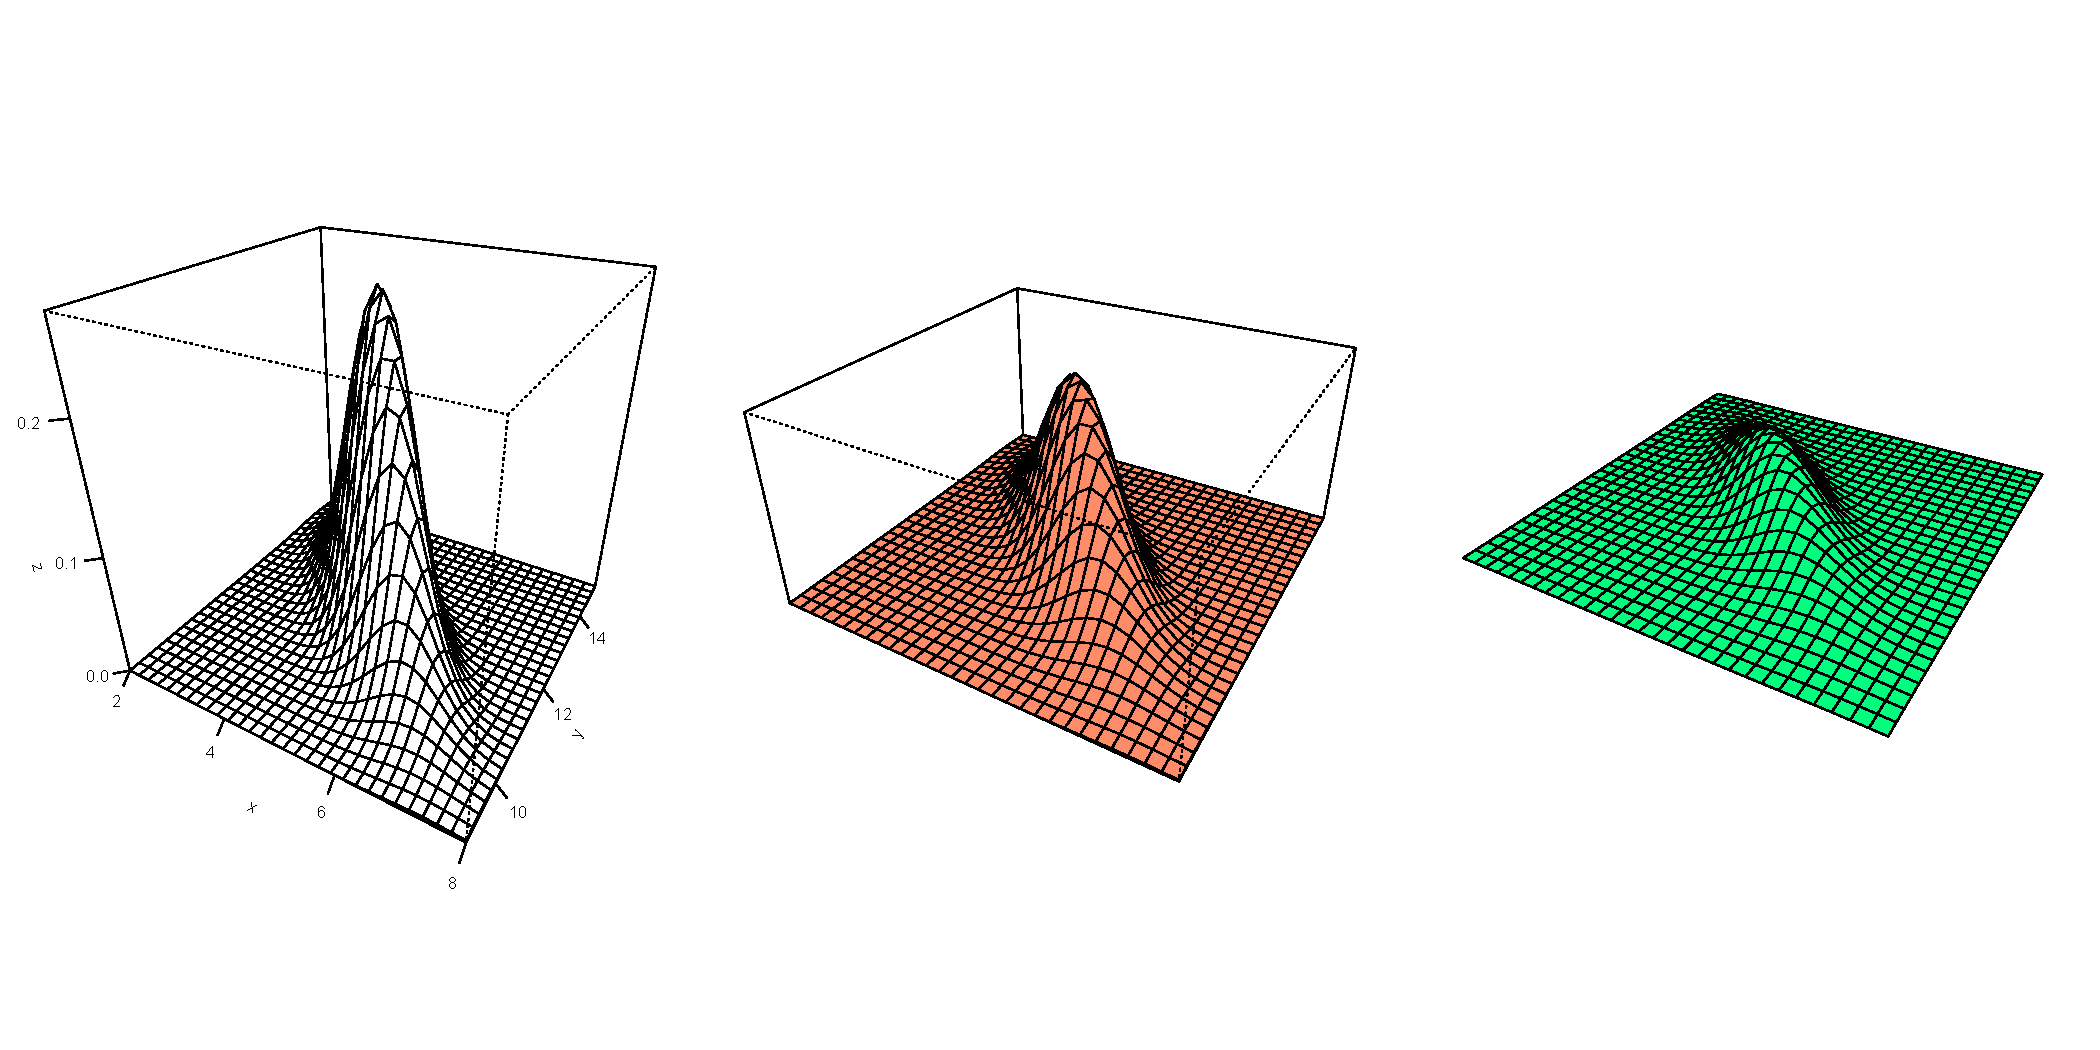
\includegraphics{Graficos_con_R_files/figure-latex/ex2persp-1.pdf}
\caption{\label{fig:ex2persp}Distribución normal bivariada.}
\end{figure}

En la Figura \ref{fig:ex2persp} se presentan las 3 perspectivas para la
densidad. Note los efectos que \texttt{ticktype}, \texttt{nticks},
\texttt{expand}, \texttt{axes} y \texttt{box} tienen sobre los dibujos
de las perspectivas.

\section{\texorpdfstring{Función \texttt{contour} \index{contour}
\index{gráfico de contornos}}{Función contour  }}\label{funcion-contour}

La función \texttt{contour} dibuja gráficos contornos. La estructura de
la función \texttt{contour} con los argumentos más usuales se muestra a
continuación:

\begin{Shaded}
\begin{Highlighting}[]
\KeywordTok{contour}\NormalTok{(x, y, z,}
\NormalTok{        xlim, ylim, zlim,}
\NormalTok{        levels, }\DataTypeTok{nlevels=}\DecValTok{20}\NormalTok{, col)}
\end{Highlighting}
\end{Shaded}

Los argumentos de la función son:

\begin{itemize}
\tightlist
\item
  \texttt{x,\ y}: vectores numéricos en los cuales se evaluó la función
  de interés para construir el objeto \texttt{z}. Ambos vectores deben
  estar ordenados.
\item
  \texttt{z}: matriz con las alturas de la función de interés, por lo
  general creada con la función \texttt{outer}.
\item
  \texttt{xlim,\ ylim,\ zlim}: límites de los ejes x, y e z
  respectivamente.
\item
  \texttt{nlevels}: número aproximado de niveles o cortes en la
  superficie a representar.
\item
  \texttt{col}: color a usar en las líneas de contornos.
\end{itemize}

La función \texttt{contour} tiene otros parámetros adicionales que el
lector puede consultar en la ayuda usando \texttt{help(contour)}.

\subsection*{Ejemplo}\label{ejemplo-21}


Generar una muestra aleatoria de 50 observaciones de una distribución
normal con parámetros \(\mu=170\) y \(\sigma^2=25\). Dibujar un gráfico
de contornos para la superficie de log-verosimilitud.

La muestra aleatoria se genera con el siguiente código.

\begin{Shaded}
\begin{Highlighting}[]
\NormalTok{y <-}\StringTok{ }\KeywordTok{rnorm}\NormalTok{(}\DataTypeTok{n=}\DecValTok{50}\NormalTok{, }\DataTypeTok{mean=}\DecValTok{170}\NormalTok{, }\DataTypeTok{sd=}\DecValTok{5}\NormalTok{)  }\CommentTok{# sd es desviación}
\end{Highlighting}
\end{Shaded}

Para dibujar los contornos solicitados se debe primero construir la
función de log-verosimilitud llamada \texttt{ll}. A continuación el
código para crear \texttt{ll}, mayores detalles de cómo construir
funciones de log-verosimilitud se pueden consultar en
\citet{hernandez_usuga}.

\begin{Shaded}
\begin{Highlighting}[]
\NormalTok{ll <-}\StringTok{ }\ControlFlowTok{function}\NormalTok{(a, b) }\KeywordTok{sum}\NormalTok{(}\KeywordTok{dnorm}\NormalTok{(}\DataTypeTok{x=}\NormalTok{y, }\DataTypeTok{mean=}\NormalTok{a, }\DataTypeTok{sd=}\NormalTok{b, }\DataTypeTok{log=}\OtherTok{TRUE}\NormalTok{))}
\NormalTok{ll <-}\StringTok{ }\KeywordTok{Vectorize}\NormalTok{(ll)  }\CommentTok{# Para vectorizar la función}
\end{Highlighting}
\end{Shaded}

Una vez construída la función \texttt{ll} se deben construir los
vectores con las coordenadas horizontal y vertical donde se evalua la
función \texttt{ll}. En el código mostrado abajo se tienen dos vectores
\texttt{xx} e \texttt{yy} obtenidos como secuencias desde el menor valor
hasta el mayor valor para cada uno de los parámetros \(\mu\) y
\(\sigma\) de la distribución normal, el valor \texttt{by=0.5} indica el
tamaño de paso de la secuencia. Luego se construye la matriz \texttt{zz}
usando la función \texttt{outer} evaluando \texttt{ll} en \texttt{xx} e
\texttt{yy}. Por último la función \texttt{contour} se aplica sobre los
elementos \texttt{xx}, \texttt{yy} e \texttt{zz}. En la Figura
\ref{fig:contour1} se muestra el gráfico de contornos con
aproximadamente 50 niveles.

\begin{Shaded}
\begin{Highlighting}[]
\NormalTok{xx <-}\StringTok{ }\KeywordTok{seq}\NormalTok{(}\DataTypeTok{from=}\DecValTok{160}\NormalTok{, }\DataTypeTok{to=}\DecValTok{180}\NormalTok{, }\DataTypeTok{by=}\FloatTok{0.5}\NormalTok{)}
\NormalTok{yy <-}\StringTok{ }\KeywordTok{seq}\NormalTok{(}\DataTypeTok{from=}\DecValTok{3}\NormalTok{, }\DataTypeTok{to=}\DecValTok{7}\NormalTok{, }\DataTypeTok{by=}\FloatTok{0.5}\NormalTok{)}
\NormalTok{zz <-}\StringTok{ }\KeywordTok{outer}\NormalTok{(}\DataTypeTok{X=}\NormalTok{xx, }\DataTypeTok{Y=}\NormalTok{yy, ll)}
\KeywordTok{contour}\NormalTok{(}\DataTypeTok{x=}\NormalTok{xx, }\DataTypeTok{y=}\NormalTok{yy, }\DataTypeTok{z=}\NormalTok{zz, }\DataTypeTok{nlevels=}\DecValTok{50}\NormalTok{,}
        \DataTypeTok{col=}\KeywordTok{gray}\NormalTok{(}\FloatTok{0.3}\NormalTok{), }\DataTypeTok{lwd=}\DecValTok{2}\NormalTok{, }\DataTypeTok{lty=}\StringTok{'solid'}\NormalTok{,}
        \DataTypeTok{xlab=}\KeywordTok{expression}\NormalTok{(mu), }\DataTypeTok{ylab=}\KeywordTok{expression}\NormalTok{(sigma))}
\end{Highlighting}
\end{Shaded}

\begin{figure}
\centering
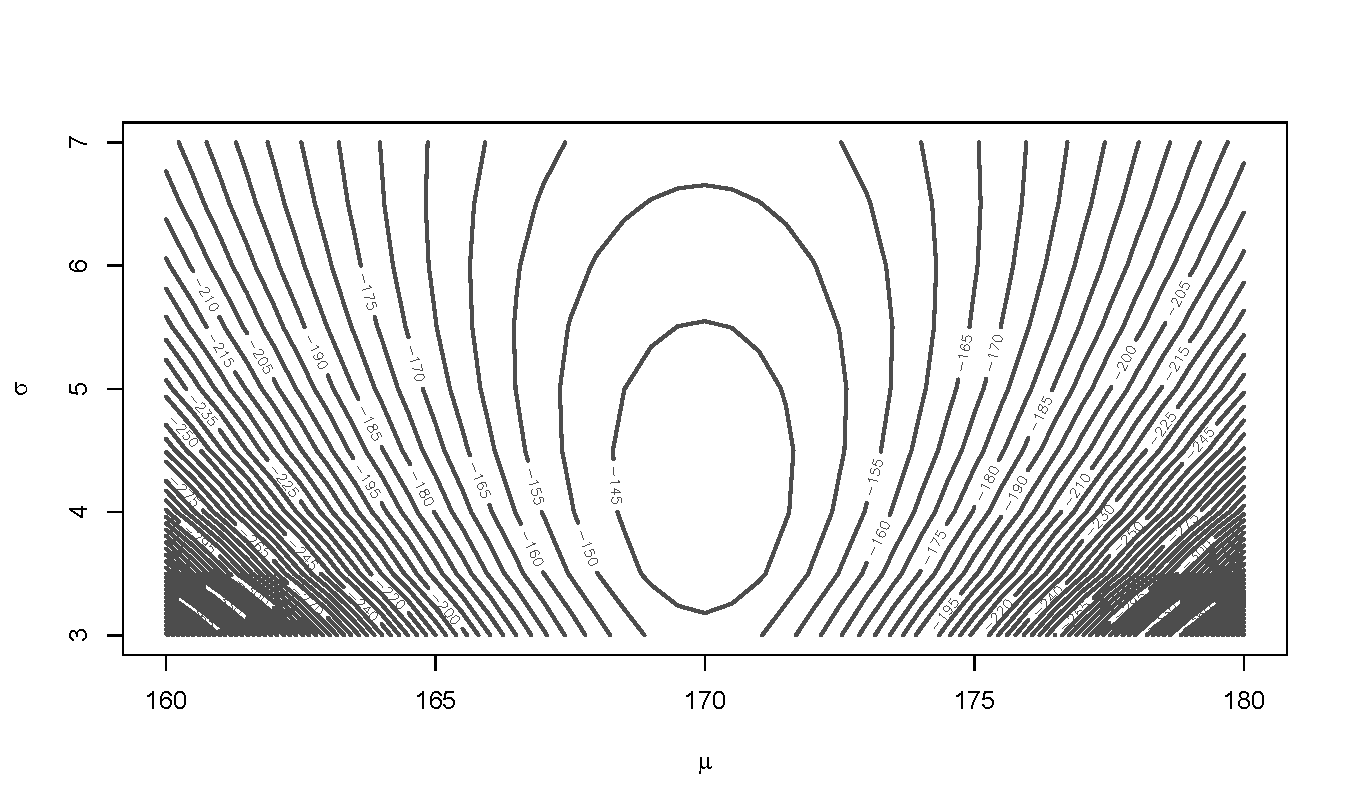
\includegraphics{Graficos_con_R_files/figure-latex/contour1-1.pdf}
\caption{\label{fig:contour1}Gráfico de contornos para la función de
log-verosimilitud para el ejemplo sobre normal.}
\end{figure}

\section{\texorpdfstring{Función \texttt{filled.contour}
\index{filled.contour}
\index{gráfico de nivel}}{Función filled.contour  }}\label{funcion-filled.contour}

La función \texttt{filled.contour} dibuja gráficos contornos pero usando
una paleta de colores. La estructura de la función
\texttt{filled.contour} con los argumentos más usuales se muestra a
continuación:

\begin{Shaded}
\begin{Highlighting}[]
\KeywordTok{filled.contour}\NormalTok{(x, y, z,}
\NormalTok{               xlim, ylim, zlim,}
\NormalTok{               levels, }\DataTypeTok{nlevels=}\DecValTok{20}\NormalTok{,}
               \DataTypeTok{color.palette=}\NormalTok{cm.colors, col)}
\end{Highlighting}
\end{Shaded}

Los argumentos de la función son:

\begin{itemize}
\tightlist
\item
  \texttt{x,\ y}: vectores numéricos en los cuales se evaluó la función
  de interés para construir el objeto \texttt{z}. Ambos vectores deben
  estar ordenados.
\item
  \texttt{z}: matriz con las alturas de la función de interés, por lo
  general creada con la función \texttt{outer}.
\item
  \texttt{xlim,\ ylim,\ zlim}: límites de los ejes x, y e z
  respectivamente.
\item
  \texttt{nlevels}: número aproximado de niveles o cortes en la
  superficie a representar.
\item
  \texttt{color.palette}: paleta de colores a usar. Por defecto es
  \texttt{cm.colors} pero el usuario puede elegir entre
  \texttt{heat.colors}, \texttt{terrain.colors} o \texttt{topo.colors}.
\end{itemize}

La función \texttt{filled.contour} tiene otros parámetros adicionales
que el lector puede consultar en la ayuda usando
\texttt{help(filled.contour)}.

\subsection*{Ejemplo}\label{ejemplo-22}


Para la muestra aleatoria obtenida en el ejemplo anterior, dibujar un
gráfico de nivel para la superficie de log-verosimilitud.

Usando los objetos \texttt{xx}, \texttt{yy} e \texttt{zz} creados en el
ejemplo anterior se puede construir el gráfico de niveles, a
continuación el código utilizado. En la Figura \ref{fig:contour2} se
muestra el gráfico de niveles con aproximadamente 20 niveles.

\begin{Shaded}
\begin{Highlighting}[]
\KeywordTok{filled.contour}\NormalTok{(}\DataTypeTok{x=}\NormalTok{xx, }\DataTypeTok{y=}\NormalTok{yy, }\DataTypeTok{z=}\NormalTok{zz, }\DataTypeTok{nlevels=}\DecValTok{20}\NormalTok{,}
               \DataTypeTok{xlab=}\KeywordTok{expression}\NormalTok{(mu), }\DataTypeTok{ylab=}\KeywordTok{expression}\NormalTok{(sigma),}
               \DataTypeTok{color =}\NormalTok{ topo.colors)}
\end{Highlighting}
\end{Shaded}

\begin{figure}
\centering
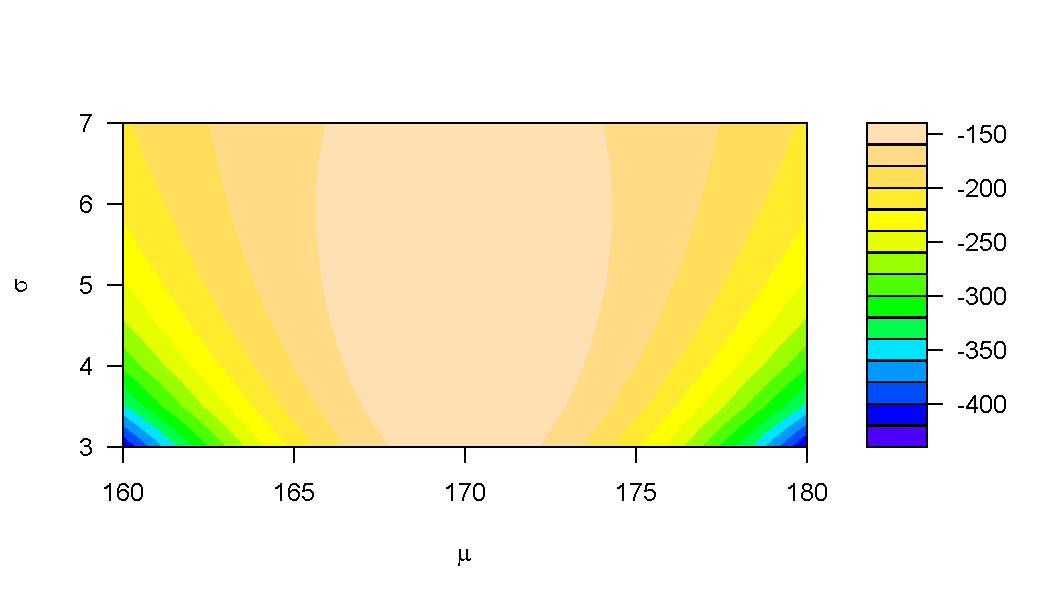
\includegraphics{Graficos_con_R_files/figure-latex/contour2-1.pdf}
\caption{\label{fig:contour2}Gráfico de nivel para la función de
log-verosimilitud para el ejemplo sobre normal.}
\end{figure}

\section{\texorpdfstring{Función \texttt{image}
\index{image}}{Función image }}\label{funcion-image}

La función \texttt{image} dibuja un gráfico de perspectiva en dos
dimensiones y visto paralelo a la tercer variable de altura, es una
especie de gráfico de calor. La estructura de la función \texttt{image}
con los argumentos más usuales se muestra a continuación:

\begin{Shaded}
\begin{Highlighting}[]
\KeywordTok{image}\NormalTok{(x, y, z)}
\end{Highlighting}
\end{Shaded}

Los argumentos de la función son:

\begin{itemize}
\tightlist
\item
  \texttt{x,\ y}: vectores numéricos en los cuales se evaluó la función
  de interés para construir el objeto \texttt{z}. Ambos vectores deben
  estar ordenados.
\item
  \texttt{z}: matriz con las alturas de la función de interés, por lo
  general creada con la función \texttt{outer}.
\end{itemize}

\subsection*{Ejemplo}\label{ejemplo-23}


Para la muestra aleatoria obtenida en el ejemplo anterior, dibujar un
gráfico con \texttt{image} para la superficie de log-verosimilitud.

Usando los objetos \texttt{xx}, \texttt{yy} e \texttt{zz} creados en el
ejemplo anterior se puede construir el gráfico solicitado, a
continuación el código utilizado. En la Figura \ref{fig:image1} se
muestra el gráfico.

\begin{Shaded}
\begin{Highlighting}[]
\KeywordTok{image}\NormalTok{(}\DataTypeTok{x=}\NormalTok{xx, }\DataTypeTok{y=}\NormalTok{yy, }\DataTypeTok{z=}\NormalTok{zz,}
      \DataTypeTok{xlab=}\KeywordTok{expression}\NormalTok{(mu), }\DataTypeTok{ylab=}\KeywordTok{expression}\NormalTok{(sigma))}
\end{Highlighting}
\end{Shaded}

\begin{figure}
\centering
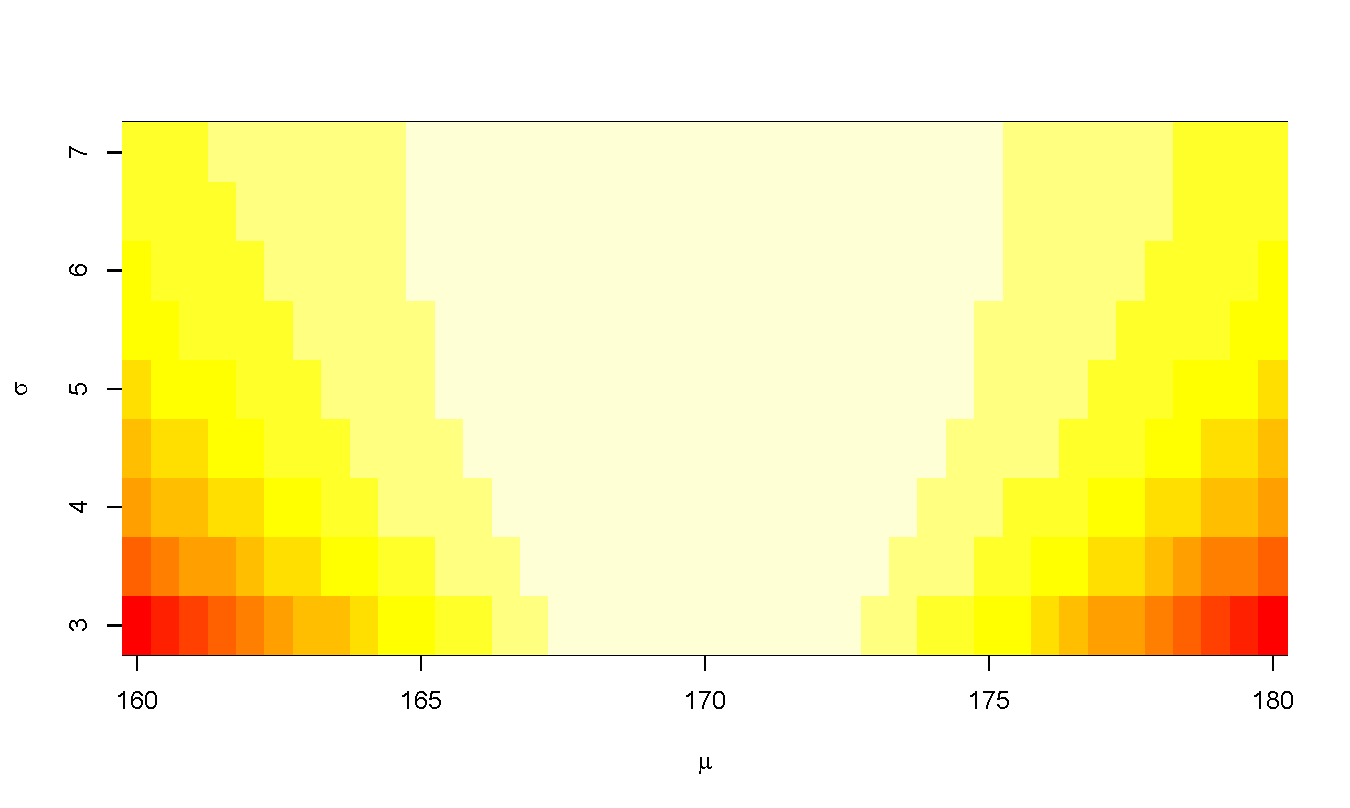
\includegraphics{Graficos_con_R_files/figure-latex/image1-1.pdf}
\caption{\label{fig:image1}Gráfico para la función de log-verosimilitud para
el ejemplo sobre normal.}
\end{figure}

\section{\texorpdfstring{Función \texttt{kde2d} \index{kde2d}
\index{densidad en 2d}}{Función kde2d  }}\label{funcion-kde2d}

La función \texttt{kde2d} pertenece al paquete \texttt{MASS} y es
utilizada para crear densidades para dos variables cuantitativas. La
estructura de la función \texttt{kde2d} con los argumentos más usuales
se muestra a continuación:

\begin{Shaded}
\begin{Highlighting}[]
\KeywordTok{kde2d}\NormalTok{(x, y, h, }\DataTypeTok{n =} \DecValTok{25}\NormalTok{, }\DataTypeTok{lims =} \KeywordTok{c}\NormalTok{(}\KeywordTok{range}\NormalTok{(x), }\KeywordTok{range}\NormalTok{(y)))}
\end{Highlighting}
\end{Shaded}

Los argumentos de la función son:

\begin{itemize}
\tightlist
\item
  \texttt{x}: vector con la variable para el eje X.
\item
  \texttt{y}: vector con la variable para el eje Y..
\item
  \texttt{h}: vector con los anchos de banda en las direcciones X e Y.
\item
  \texttt{n}: número de puntos para construir la rejilla.
\item
  \texttt{lims}: límites del rectángulo de datos a considerar, debe ser
  un vector de la forma \texttt{c(xl,\ xu,\ yl,\ yu)}. Este parámetro
  por defecto es \texttt{c(range(x),\ range(y))}.
\end{itemize}

\subsection*{Ejemplo}\label{ejemplo-24}


La base de datos medidas del cuerpo cuenta con 6 variables registradas a
un grupo de 36 estudiantes de la universidad, dos de esas variables son
la altura y el peso corporal. Se desea construir un gráfico de densidad
bivariada para altura y peso.

El código mostrado a continuación hace la lectura de la base de datos y
luego se construyen dos densidades, la primera con \texttt{n=5} y la
segunda con \texttt{n=50}, esto para ver el efecto del parámetro
\texttt{n}.

\begin{Shaded}
\begin{Highlighting}[]
\NormalTok{url <-}\StringTok{ 'https://raw.githubusercontent.com/fhernanb/datos/master/medidas_cuerpo'}
\NormalTok{datos <-}\StringTok{ }\KeywordTok{read.table}\NormalTok{(}\DataTypeTok{file=}\NormalTok{url, }\DataTypeTok{header=}\NormalTok{T)}

\KeywordTok{require}\NormalTok{(MASS)  }\CommentTok{# Se debe cargar este paquete}
\NormalTok{f1 <-}\StringTok{ }\KeywordTok{kde2d}\NormalTok{(}\DataTypeTok{x=}\NormalTok{datos}\OperatorTok{$}\NormalTok{peso, }\DataTypeTok{y=}\NormalTok{datos}\OperatorTok{$}\NormalTok{altura, }\DataTypeTok{n=}\DecValTok{5}\NormalTok{)}
\NormalTok{f2 <-}\StringTok{ }\KeywordTok{kde2d}\NormalTok{(}\DataTypeTok{x=}\NormalTok{datos}\OperatorTok{$}\NormalTok{peso, }\DataTypeTok{y=}\NormalTok{datos}\OperatorTok{$}\NormalTok{altura, }\DataTypeTok{n=}\DecValTok{50}\NormalTok{)}
\end{Highlighting}
\end{Shaded}

En el código mostrado a continuación se dibujan las dos densidades
usando un gráfico de calor usando la función \texttt{image}.

\begin{Shaded}
\begin{Highlighting}[]
\KeywordTok{par}\NormalTok{(}\DataTypeTok{mfrow=}\KeywordTok{c}\NormalTok{(}\DecValTok{1}\NormalTok{, }\DecValTok{2}\NormalTok{))}
\KeywordTok{image}\NormalTok{(f1, }\DataTypeTok{xlab=}\StringTok{'Peso'}\NormalTok{, }\DataTypeTok{ylab=}\StringTok{'Estatura'}\NormalTok{, }\DataTypeTok{main=}\StringTok{'n=5'}\NormalTok{)}
\KeywordTok{image}\NormalTok{(f2, }\DataTypeTok{xlab=}\StringTok{'Peso'}\NormalTok{, }\DataTypeTok{ylab=}\StringTok{'Estatura'}\NormalTok{, }\DataTypeTok{main=}\StringTok{'n=50'}\NormalTok{)}
\end{Highlighting}
\end{Shaded}

\begin{figure}
\centering
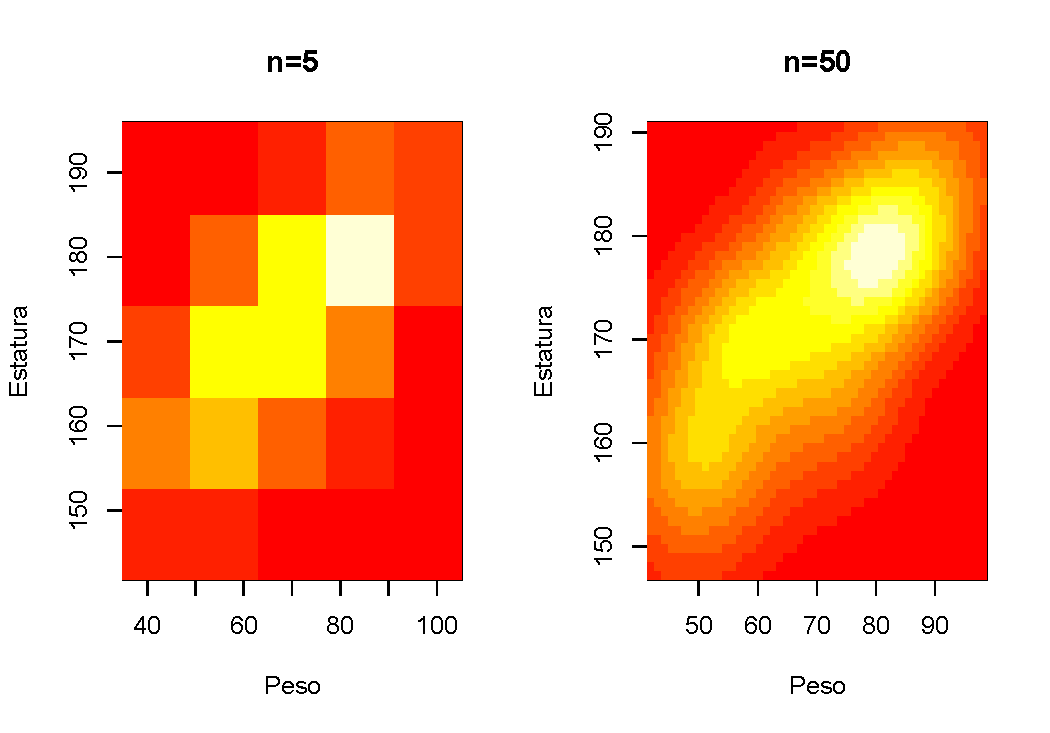
\includegraphics{Graficos_con_R_files/figure-latex/den2d1-1.pdf}
\caption{\label{fig:den2d1}Gráfico de densidad bivariada para el peso
corporal y la estatura de un grupo de estudiantes. A la izquierda la
densidad con \texttt{n=5} y a la derecha con \texttt{n=50}.}
\end{figure}

\section{\texorpdfstring{Función \texttt{interaction.plot}
\index{interaction.plot}
\index{gráfico de interacción}}{Función interaction.plot  }}\label{funcion-interaction.plot}

La función \texttt{interaction.plot} dibuja gráficos de interacción. La
estructura de la función \texttt{interaction.plot} con los argumentos
más usuales se muestra a continuación:

\begin{Shaded}
\begin{Highlighting}[]
\KeywordTok{interaction.plot}\NormalTok{(response, x.factor, trace.factor, fun,}
\NormalTok{                 legend, trace.label)}
\end{Highlighting}
\end{Shaded}

Los argumentos de la función son:

\begin{itemize}
\tightlist
\item
  \texttt{response}: vector numérico con la variable respuesta.
\item
  \texttt{x.factor}: factor 1 a ubicar en el eje horizontal.
\item
  \texttt{trace.factor}: factor 2 para diferenciar las líneas.
\item
  \texttt{fun}: función a aplicar para a \texttt{response} para cada
  combinación de \texttt{x.factor} y \texttt{trace.factor}.
\item
  \texttt{legend}: valor lógico para incluir o no leyenda.
\item
  \texttt{trace.label}: nombre a colocar en la leyenda.
\end{itemize}

La función \texttt{interaction.plot} tiene otros parámetros adicionales
que el lector puede consultar en la ayuda usando
\texttt{help(interaction.plot)}.

\subsection*{Ejemplo}\label{ejemplo-25}


Se realizó un experimento para determinar cómo influye el material de la
batería y la temperatura del medio ambiente sobre la duración en horas
de la batería. Se desea construir un gráfico de interacción entre
Temperatura y Material para ver el efecto sobre la duración promedio de
las baterías. Los datos y el código para generar el gráfico solicitado
se muestran a continuación.

\begin{Shaded}
\begin{Highlighting}[]
\NormalTok{horas <-}\StringTok{ }\KeywordTok{c}\NormalTok{(}\DecValTok{130}\NormalTok{, }\DecValTok{155}\NormalTok{, }\DecValTok{74}\NormalTok{, }\DecValTok{180}\NormalTok{, }\DecValTok{150}\NormalTok{, }\DecValTok{188}\NormalTok{, }\DecValTok{159}\NormalTok{, }\DecValTok{126}\NormalTok{, }\DecValTok{138}\NormalTok{, }\DecValTok{110}\NormalTok{, }\DecValTok{168}\NormalTok{, }
           \DecValTok{160}\NormalTok{, }\DecValTok{34}\NormalTok{, }\DecValTok{40}\NormalTok{, }\DecValTok{80}\NormalTok{, }\DecValTok{75}\NormalTok{, }\DecValTok{136}\NormalTok{, }\DecValTok{122}\NormalTok{, }\DecValTok{106}\NormalTok{, }\DecValTok{115}\NormalTok{, }\DecValTok{174}\NormalTok{, }\DecValTok{120}\NormalTok{, }\DecValTok{150}\NormalTok{, }
           \DecValTok{139}\NormalTok{, }\DecValTok{20}\NormalTok{, }\DecValTok{70}\NormalTok{, }\DecValTok{82}\NormalTok{, }\DecValTok{58}\NormalTok{, }\DecValTok{25}\NormalTok{, }\DecValTok{70}\NormalTok{, }\DecValTok{58}\NormalTok{, }\DecValTok{45}\NormalTok{, }\DecValTok{96}\NormalTok{, }\DecValTok{104}\NormalTok{, }\DecValTok{82}\NormalTok{, }\DecValTok{60}\NormalTok{)}

\NormalTok{temperatura <-}\StringTok{ }\KeywordTok{rep}\NormalTok{(}\KeywordTok{c}\NormalTok{(}\DecValTok{15}\NormalTok{, }\DecValTok{70}\NormalTok{, }\DecValTok{125}\NormalTok{), }\DataTypeTok{each=}\DecValTok{12}\NormalTok{)}
\NormalTok{material    <-}\StringTok{ }\KeywordTok{rep}\NormalTok{(}\DecValTok{1}\OperatorTok{:}\DecValTok{3}\NormalTok{, }\DataTypeTok{each=}\DecValTok{4}\NormalTok{, }\DataTypeTok{times=}\DecValTok{3}\NormalTok{)}

\KeywordTok{interaction.plot}\NormalTok{(}\DataTypeTok{x.factor=}\NormalTok{temperatura, }\DataTypeTok{trace.factor=}\NormalTok{material,}
                 \DataTypeTok{response=}\NormalTok{horas, }\DataTypeTok{trace.label=}\StringTok{'Material'}\NormalTok{,}
                 \DataTypeTok{xlab=}\StringTok{'Temperatura'}\NormalTok{,}
                 \DataTypeTok{ylab=}\StringTok{'Duración promedio (horas)'}\NormalTok{,}
                 \DataTypeTok{col=}\KeywordTok{c}\NormalTok{(}\StringTok{'blue'}\NormalTok{, }\StringTok{'black'}\NormalTok{, }\StringTok{'red'}\NormalTok{),}
                 \DataTypeTok{fun=}\NormalTok{mean, }\DataTypeTok{lwd=}\DecValTok{3}\NormalTok{, }\DataTypeTok{las=}\DecValTok{1}\NormalTok{, }\DataTypeTok{fixed=}\NormalTok{T)}
\end{Highlighting}
\end{Shaded}

\begin{figure}
\centering
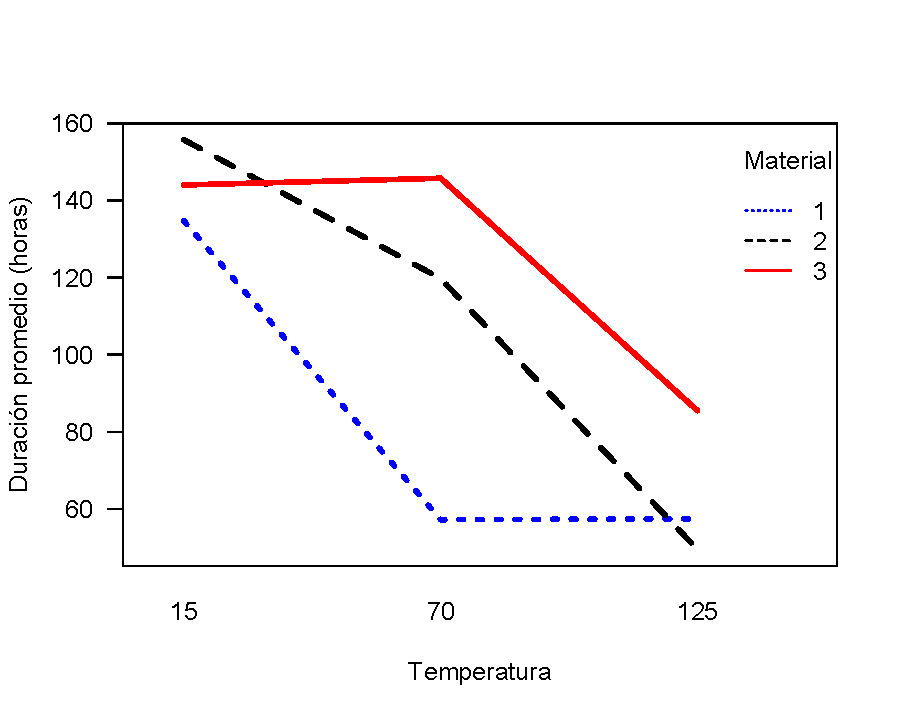
\includegraphics{Graficos_con_R_files/figure-latex/intplot1-1.pdf}
\caption{\label{fig:intplot1}Gráfico de interacción entre Temperatura y
Material sobre la duración promedio de las baterías.}
\end{figure}

\section{\texorpdfstring{Gráfico de espagueti
\index{espagueti}}{Gráfico de espagueti }}\label{grafico-de-espagueti}

Los gráficos de espagueti son usados para representar la evolución de
una variable medida para un grupo de sujetos en diferentes momentos del
tiempo. La función \texttt{interaction.plot} se puede usar para obtener
este tipo de gráficos, a continuación un ejemplo.

\subsection*{Ejemplo}\label{ejemplo-26}


El ejemplo aquí presentado fue tomado de este
\href{http://stats.idre.ucla.edu/r/faq/how-can-i-make-spaghetti-plots/}{enlace}.
El objetivo es crear un gráfico de espagueti para mostrar la evolución
de la variable tolerancia a través del tiempo para cada uno de los 16
individuos estudiados. El código para descargar la base de datos y
construir el gráfico se muestran a continuación.

\begin{Shaded}
\begin{Highlighting}[]
\NormalTok{dt <-}\StringTok{ }\KeywordTok{read.table}\NormalTok{(}\StringTok{"https://stats.idre.ucla.edu/stat/r/faq/tolpp.csv"}\NormalTok{,}
                 \DataTypeTok{sep=}\StringTok{","}\NormalTok{, }\DataTypeTok{header=}\NormalTok{T)}

\KeywordTok{interaction.plot}\NormalTok{(}\DataTypeTok{response=}\NormalTok{dt}\OperatorTok{$}\NormalTok{tolerance,}
                 \DataTypeTok{x.factor=}\NormalTok{dt}\OperatorTok{$}\NormalTok{time, }\DataTypeTok{col=}\DecValTok{1}\OperatorTok{:}\DecValTok{8}\NormalTok{, }\DataTypeTok{lwd=}\DecValTok{2}\NormalTok{,}
                 \DataTypeTok{trace.factor=}\NormalTok{dt}\OperatorTok{$}\NormalTok{id, }\DataTypeTok{las=}\DecValTok{1}\NormalTok{, }\DataTypeTok{lty=}\DecValTok{1}\NormalTok{, }
                 \DataTypeTok{xlab=}\StringTok{"Tiempo"}\NormalTok{, }\DataTypeTok{ylab=}\StringTok{"Tolerancia"}\NormalTok{, }\DataTypeTok{legend=}\NormalTok{F)}
\end{Highlighting}
\end{Shaded}

\begin{figure}
\centering
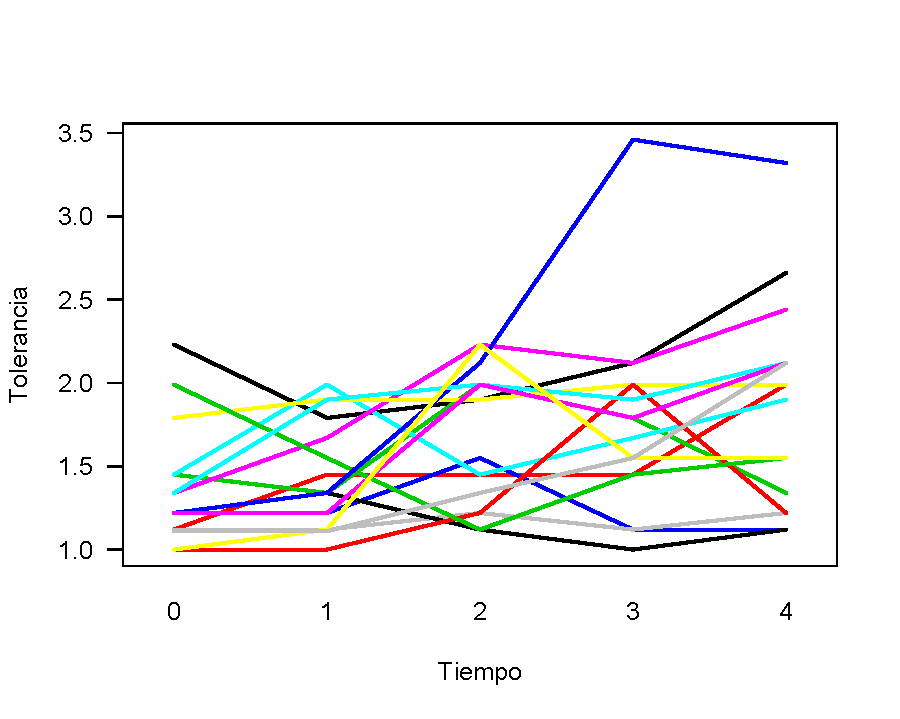
\includegraphics{Graficos_con_R_files/figure-latex/intplot2-1.pdf}
\caption{\label{fig:intplot2}Gráfico de espagueti para ver la evolución de
la variable tolerancia.}
\end{figure}

\chapter{Gráficos para variables
cualitativas}\label{graficos-para-variables-cualitativas}

En este capítulo se presentan funciones para la creación de gráficos
para variables cualitativas.

\section{\texorpdfstring{Función \texttt{barplot}
\index{gráfico de barras}
\index{barplot}}{Función barplot  }}\label{funcion-barplot}

Los gráficos de barras son útiles para representar las frecuencias
absolutas o relativas asociadas a los niveles de una variable
cualitativa y la función \texttt{barplot} se usa para obtener un gráfico
de barras. La estructura de la función \texttt{barplot} con los
argumentos más comunes de uso se muestra a continuación.

\begin{Shaded}
\begin{Highlighting}[]
\KeywordTok{barplot}\NormalTok{(height, beside, horiz)}
\end{Highlighting}
\end{Shaded}

Los argumentos de la función \texttt{barplot} son:

\begin{itemize}
\tightlist
\item
  \texttt{height}: vector o matriz con la información de las frecuencias
  absolutas o relativas.
\item
  \texttt{beside}: valor lógico para indicar si las barras deben estar
  al lado cuando la información ingresada es una matriz.
\item
  \texttt{horiz}: valor lógico para indicar si el diagrama de barras
  debe ser horizontal, por defecto es \texttt{FALSE}.
\end{itemize}

La función \texttt{barplot} tiene otros parámetros que pueden ser
consultados en la ayuda de la función por medio de la instrucción
\texttt{?barplot}.

\subsection*{Ejemplo}\label{ejemplo-27}


Suponga que queremos construir un diagrama de barras para las
frecuencias relativas de la variable estrato socioeconómico del
apartamento de la base de datos sobre apartamentos usados en Medellín.

A continuación se muestra el código necesario para cargar la base de
datos \texttt{aptos2015}. Antes de construir el diagrama de barras
solicitado es necesario construir la tabla de frecuencias para la
variable estrato, para esto se usa la función \texttt{table} y los
resultados se almacenan en el objeto \texttt{tabla1} que contiene las
frecuencias \textbf{absolutas}. Para obtener las frecuencias
\textbf{relativas} se usa luego la función \texttt{prop.table} sobre el
objeto \texttt{tabla1}.

\begin{Shaded}
\begin{Highlighting}[]
\NormalTok{url <-}\StringTok{ 'https://raw.githubusercontent.com/fhernanb/datos/master/aptos2015'}
\NormalTok{datos <-}\StringTok{ }\KeywordTok{read.table}\NormalTok{(}\DataTypeTok{file=}\NormalTok{url, }\DataTypeTok{header=}\NormalTok{T)}
\NormalTok{tabla1 <-}\StringTok{ }\KeywordTok{table}\NormalTok{(datos}\OperatorTok{$}\NormalTok{estrato)}
\NormalTok{tabla1 <-}\StringTok{ }\KeywordTok{prop.table}\NormalTok{(tabla1)}
\NormalTok{tabla1}
\end{Highlighting}
\end{Shaded}

\begin{verbatim}
## 
##       2       3       4       5       6 
## 0.01153 0.23199 0.19885 0.20893 0.34870
\end{verbatim}

Una vez se tiene el objeto con la información de las frecuencias
relativas se puede dibujar el diagrama de barras usando el siguiente
código.

\begin{Shaded}
\begin{Highlighting}[]
\KeywordTok{barplot}\NormalTok{(tabla1, }\DataTypeTok{xlab=}\StringTok{'Estrato socioeconómico',}
\StringTok{        ylab='}\NormalTok{Frecuencia relativa}\StringTok{', las=1)}
\end{Highlighting}
\end{Shaded}

\begin{figure}
\centering
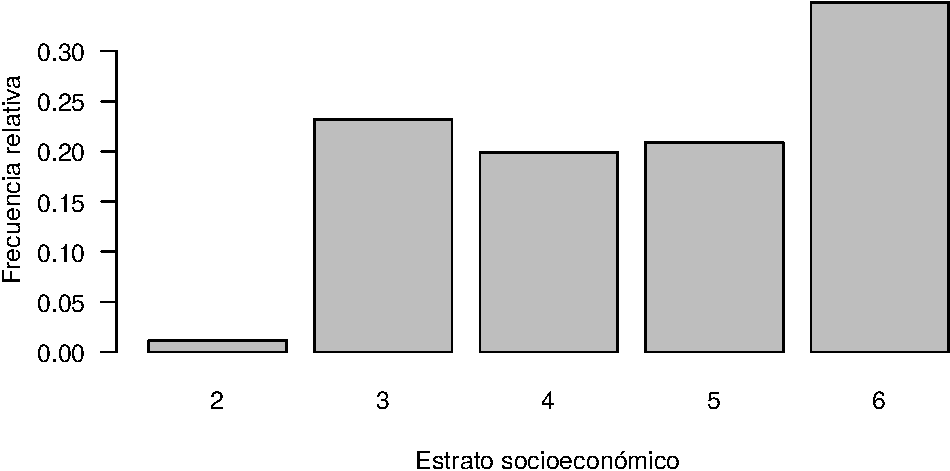
\includegraphics{Graficos_con_R_files/figure-latex/barra1-1.pdf}
\caption{\label{fig:barra1}Diagrama de barras para el estrato socioeconómico
de los apartamentos usados.}
\end{figure}

En la Figura \ref{fig:barra1} se presenta el diagrama de barras
solicitado. Se observa que hay pocos apartamentos (1.15\%)
pertenecientes al estrato dos, los estratos tres, cuatro y cinco aportan
porcentajes similares a la base de datos y que el estrato 6 es el que
más apartamentos aporta a la base de datos, 34.87\%.

Algunas veces se acostumbra a colocar las frecuencias relativas sobre la
parte superior de las barras para facilitar la lectura. A continuación
se presenta el código para replicar la Figura \ref{fig:barra1} con las
frecuencias relativas. Lo primero que se hace es dibujar el diagrama de
barras y almacenar la información de él en el objeto \texttt{xx} para
luego poder usar la ubicación de cada una de las barras. Note que se
agregó también \texttt{ylim=c(0,\ 0.45)} para conseguir una ampliación
del eje vertical, esto para lograr que se vea el número sobre la barra
del estrato 6. Luego se usa la función \texttt{text} para incluir un
texto en las coordenadas \texttt{x=xx} y \texttt{y=tabla1}, el parámetro
\texttt{pos=3} coloca el texto en la parte superior de las coordenadas y
el parámetro \texttt{label} sirve para indicar lo que se desea escribir
en las coordenadas indicadas, en este caso son las frecuencias relativas
almacenadas en \texttt{tabla1}.

\begin{Shaded}
\begin{Highlighting}[]
\NormalTok{xx <-}\StringTok{ }\KeywordTok{barplot}\NormalTok{(tabla1, }\DataTypeTok{ylim=}\KeywordTok{c}\NormalTok{(}\DecValTok{0}\NormalTok{, }\FloatTok{0.45}\NormalTok{), }\DataTypeTok{col=}\KeywordTok{gray}\NormalTok{(}\FloatTok{0.9}\NormalTok{),}
              \DataTypeTok{xlab=}\StringTok{'Estrato socioeconómico',}
\StringTok{              ylab='}\NormalTok{Frecuencia relativa}\StringTok{', las=1)}

\StringTok{text(x=xx, y=tabla1, pos=3, cex=0.8, col="red",}
\StringTok{     label=round(tabla1, 4))}
\end{Highlighting}
\end{Shaded}

\begin{figure}
\centering
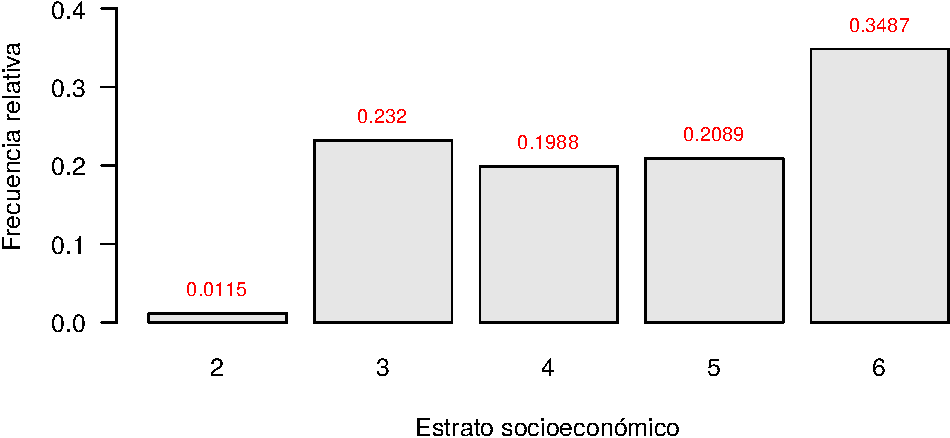
\includegraphics{Graficos_con_R_files/figure-latex/barra2-1.pdf}
\caption{\label{fig:barra2}Diagrama de barras para el estrato socioeconómico
de los apartamentos usados con las frecuencias relativas sobre las
barras.}
\end{figure}

En la Figura \ref{fig:barra2} se muestra el diagrama de barras
modificado. Note que si no se hubiese usado \texttt{ylim=c(0,\ 0.45)} al
dibujar el diagrama, la marca sobre la última barra no se podría ver.

\subsection*{Ejemplo}\label{ejemplo-28}


Suponga que queremos construir un diagrama de barras para comparar la
variable presencia de parqueadero con el estrato socioeconómico en la
base de datos sobre apartamentos usados en Medellín.

La función \texttt{barplot} también puede ser usada para representar una
tabla de frecuencia con dos variables. Para obtener la tabla de
frecuencia para relacionar parqueadero con estrato se usa el siguiente
código.

\begin{Shaded}
\begin{Highlighting}[]
\NormalTok{tabla2 <-}\StringTok{ }\KeywordTok{table}\NormalTok{(datos}\OperatorTok{$}\NormalTok{parqueadero, datos}\OperatorTok{$}\NormalTok{estrato)}
\NormalTok{tabla2}
\end{Highlighting}
\end{Shaded}

\begin{verbatim}
##     
##        2   3   4   5   6
##   no   5  88  24   8   1
##   si   3  73 114 137 241
\end{verbatim}

El anterior resultado es la tabla de contingencia entre las variables
parqueadero y estrato, de esta tabla vemos que para estratos superiores
el número de apartamentos que si tienen parqueadero es mayor que los
apartamentos sin parqueadero. La tabla anterior se puede representar
gráficamente usando el siguiente código.

\begin{Shaded}
\begin{Highlighting}[]
\KeywordTok{barplot}\NormalTok{(tabla2)}
\end{Highlighting}
\end{Shaded}

\begin{figure}
\centering
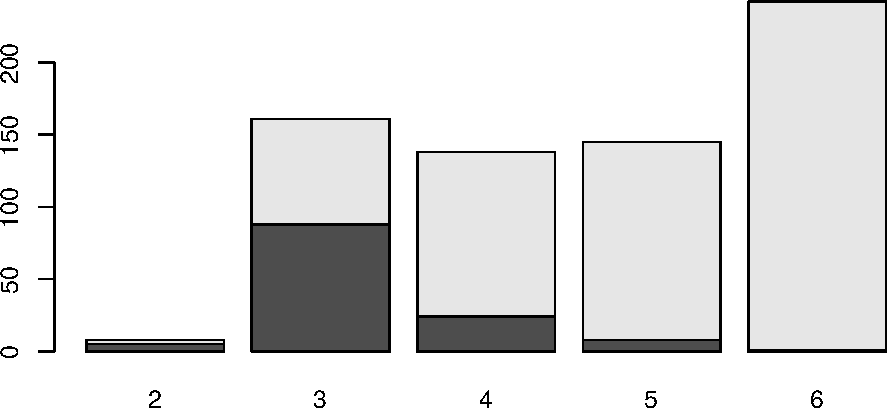
\includegraphics{Graficos_con_R_files/figure-latex/barra3-1.pdf}
\caption{\label{fig:barra3}Diagrama I de barras la relación entre
parqueadero y estrato.}
\end{figure}

En la Figura \ref{fig:barra3} se muestra el gráfico de barras sin
editar, el color negro representa la frecuencia de los apartamentos sin
parqueadero (no) y el color gris representa los apartamentos con
parqueadero (si), las barras están una encima de la otra y la
comparación no es tan clara como debería. Para mejorar la comparación se
usa el parámetro \texttt{besides=TRUE}, a continuación el código
utilizado.

\begin{Shaded}
\begin{Highlighting}[]
\KeywordTok{barplot}\NormalTok{(tabla2, }\DataTypeTok{beside=}\OtherTok{TRUE}\NormalTok{)}
\end{Highlighting}
\end{Shaded}

\begin{figure}
\centering
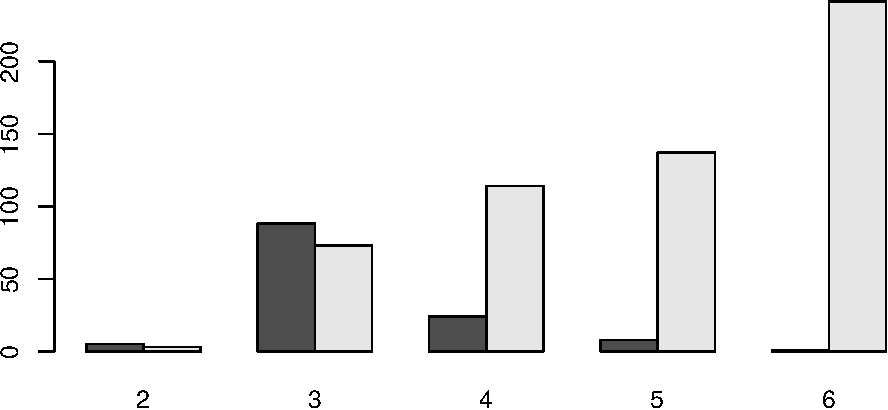
\includegraphics{Graficos_con_R_files/figure-latex/barra4-1.pdf}
\caption{\label{fig:barra4}Diagrama II de barras la relación entre
parqueadero y estrato.}
\end{figure}

En la Figura \ref{fig:barra4} está el gráfico de barras obtenido
agregando \texttt{besides=TRUE} para que las barras se ubiquen una junto
a la otra. Este gráfico se puede mejorar aún más colocando una leyenda
para identificar las barras, nombrando los ejes y usando otros colores,
a continuación el código utilizado.

\begin{Shaded}
\begin{Highlighting}[]
\KeywordTok{barplot}\NormalTok{(tabla2, }\DataTypeTok{beside =} \OtherTok{TRUE}\NormalTok{, }\DataTypeTok{las=}\DecValTok{1}\NormalTok{, }
        \DataTypeTok{xlab=}\StringTok{'Estrato'}\NormalTok{, }\DataTypeTok{ylab=}\StringTok{'Frecuencia'}\NormalTok{,}
        \DataTypeTok{col =} \KeywordTok{c}\NormalTok{(}\StringTok{"lightblue"}\NormalTok{, }\StringTok{"mistyrose"}\NormalTok{),}
        \DataTypeTok{ylim =} \KeywordTok{c}\NormalTok{(}\DecValTok{0}\NormalTok{, }\DecValTok{250}\NormalTok{))}
\KeywordTok{legend}\NormalTok{(}\StringTok{'topleft'}\NormalTok{, }\DataTypeTok{legend=}\KeywordTok{rownames}\NormalTok{(tabla2), }\DataTypeTok{bty=}\StringTok{'n'}\NormalTok{,}
       \DataTypeTok{fill=}\KeywordTok{c}\NormalTok{(}\StringTok{"lightblue"}\NormalTok{, }\StringTok{"mistyrose"}\NormalTok{))}
\end{Highlighting}
\end{Shaded}

\begin{figure}
\centering
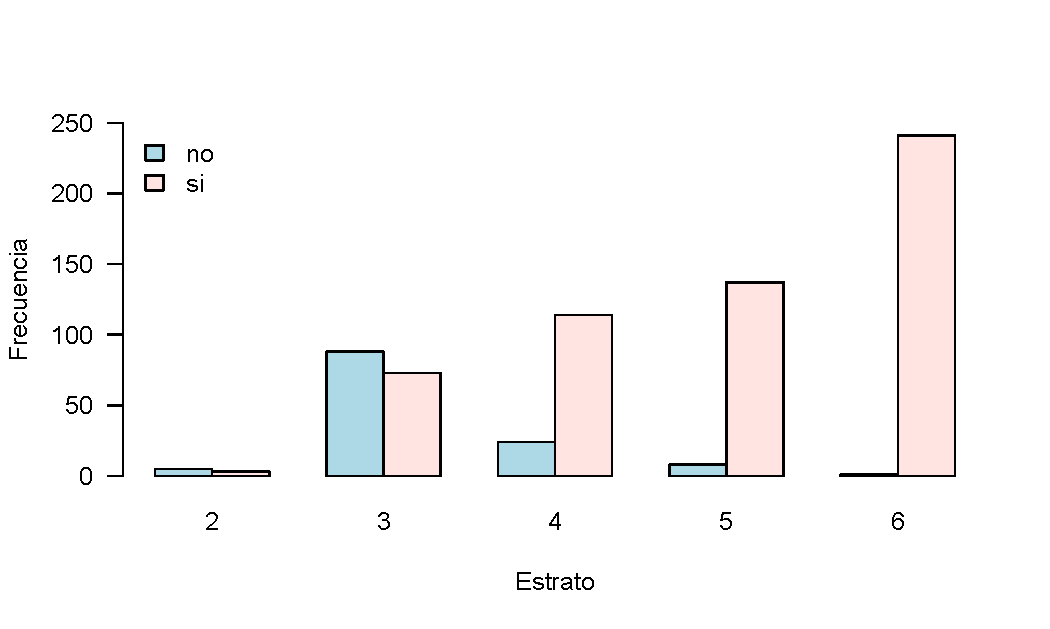
\includegraphics{Graficos_con_R_files/figure-latex/barra5-1.pdf}
\caption{\label{fig:barra5}Relación entre la presencia de parqueadero y el
estrato socioeconómico.}
\end{figure}

En la Figura \ref{fig:barra5} se observa el gráfico de barras
solicitado, se observa claramente que en los estratos 4, 5 y 6
predominan los aparatamentos con parqueadero.

Es posible construir una tabla de contingencia de frecuencia relativa
para ver cómo es el comportamiento de tener o no parquedadero dentro de
cada estrato, el siguiente código construye la \texttt{tabla3} con la
información necesaria. La función \texttt{prop.table} permite obtener la
tabla de frecuencias \textbf{relativas} a partir de una tabla de
frecuencias absolutas, el parámetro \texttt{margin} sirve para indicar
si las frecuencias \textbf{relativas} se deben obtener por fila
(\texttt{margin=1}) o por columnas (\texttt{margin=2}).

\begin{Shaded}
\begin{Highlighting}[]
\NormalTok{tabla3 <-}\StringTok{ }\KeywordTok{prop.table}\NormalTok{(tabla2, }\DataTypeTok{margin=}\DecValTok{2}\NormalTok{)}
\NormalTok{tabla3}
\end{Highlighting}
\end{Shaded}

\begin{verbatim}
##     
##             2        3        4        5        6
##   no 0.625000 0.546584 0.173913 0.055172 0.004132
##   si 0.375000 0.453416 0.826087 0.944828 0.995868
\end{verbatim}

De la anterior tabla se ve que el porcentaje de apartamentos con
parqueadero supera enormemente el los apartamentos sin parqueadero para
los estratos 6, 5 y 4. El código para generar un gráfico asociado a la
\texttt{tabla3} se muestra a continuación.

\begin{Shaded}
\begin{Highlighting}[]
\KeywordTok{barplot}\NormalTok{(tabla3, }
        \DataTypeTok{beside =} \OtherTok{TRUE}\NormalTok{, }\DataTypeTok{las=}\DecValTok{1}\NormalTok{, }
        \DataTypeTok{xlab=}\StringTok{'Estrato'}\NormalTok{, }\DataTypeTok{ylab=}\StringTok{'Frecuencia relativa'}\NormalTok{,}
        \DataTypeTok{col =} \KeywordTok{c}\NormalTok{(}\StringTok{"lightblue"}\NormalTok{, }\StringTok{"mistyrose"}\NormalTok{),}
        \DataTypeTok{ylim =} \KeywordTok{c}\NormalTok{(}\DecValTok{0}\NormalTok{, }\DecValTok{1}\NormalTok{))}
\KeywordTok{legend}\NormalTok{(}\StringTok{'topleft'}\NormalTok{, }\DataTypeTok{legend=}\KeywordTok{rownames}\NormalTok{(tabla2), }\DataTypeTok{bty=}\StringTok{'n'}\NormalTok{,}
       \DataTypeTok{fill=}\KeywordTok{c}\NormalTok{(}\StringTok{"lightblue"}\NormalTok{, }\StringTok{"mistyrose"}\NormalTok{))}
\end{Highlighting}
\end{Shaded}

\begin{figure}
\centering
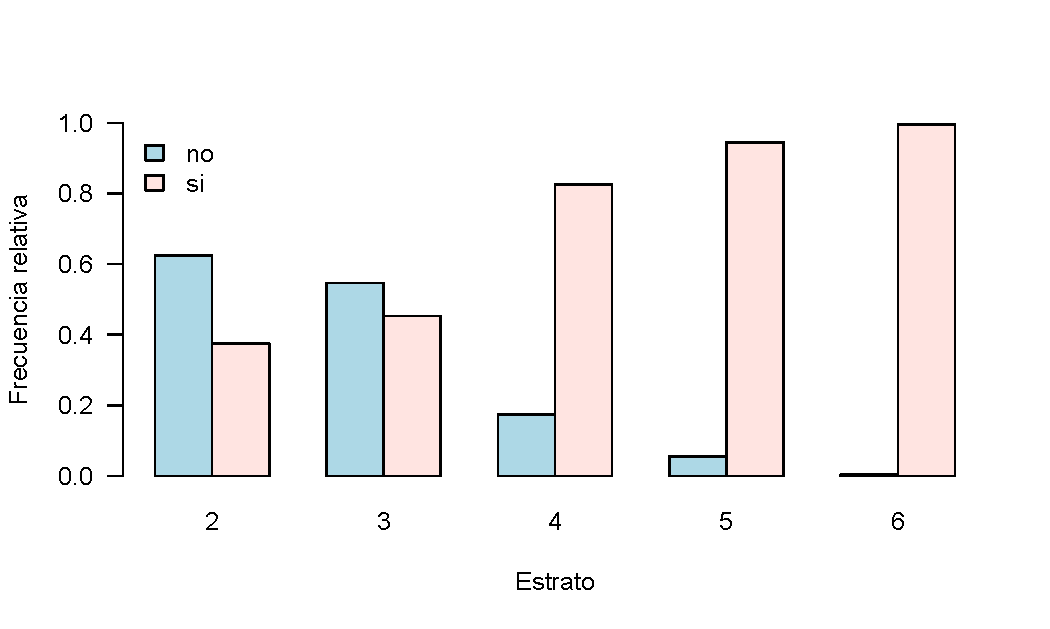
\includegraphics{Graficos_con_R_files/figure-latex/barra6-1.pdf}
\caption{\label{fig:barra6}Relación entre la presencia de parqueadero y el
estrato socioeconómico.}
\end{figure}

¿Cuáles son las ventajas y/o desventajas de las figuras \ref{fig:barra5}
y \ref{fig:barra6} al ser presentadas en un informe?

\section{\texorpdfstring{Función \texttt{pie} \index{gráfico de pastel}
\index{pie}}{Función pie  }}\label{funcion-pie}

En \proglang{R} es posible construir gráficos de pastel para representar
una tabla de frecuencia relativa o absoluta, sin embargo este tipo de
gráficos no es recomendable y en la ayuda de la función se hace la
siguiente advertencia:

\BeginKnitrBlock{rmdwarning}
Pie charts are a very bad way of displaying information. The eye is good
at judging linear measures and bad at judging relative areas. A bar
chart or dot chart is a preferable way of displaying this type of data.
\EndKnitrBlock{rmdwarning}

La estructura de la función \texttt{pie} con los argumentos más comunes
de uso se muestra a continuación.

\begin{Shaded}
\begin{Highlighting}[]
\KeywordTok{pie}\NormalTok{(x, labels)}
\end{Highlighting}
\end{Shaded}

Los argumentos de la función \texttt{pie} son:

\begin{itemize}
\tightlist
\item
  \texttt{x}: vector con elementos no negativos que representan las
  frecuencias de los niveles de la variable cualitativa.
\item
  \texttt{labels}: vector con los nombres a colocar en cada parte del
  pastel, por defecto se usan los nombres del vector \texttt{x}.
\end{itemize}

\subsection*{Ejemplo}\label{ejemplo-29}


Dibujar un gráfico de pastel para las frecuencias relativas de la
variable estrato socioeconómico del apartamento de la base de datos
sobre apartamentos usados en Medellín.

La \texttt{tabla1} construída en el primer ejemplo de \texttt{barplot}
se utiliza para construir el gráfico solicitado. Abajo el código
necesario para construir el gráfico.

\begin{Shaded}
\begin{Highlighting}[]
\NormalTok{nombres <-}\StringTok{ }\KeywordTok{paste}\NormalTok{(}\StringTok{'Estrato '}\NormalTok{, }\DecValTok{2}\OperatorTok{:}\DecValTok{6}\NormalTok{)}
\KeywordTok{pie}\NormalTok{(}\DataTypeTok{x=}\NormalTok{tabla1, }\DataTypeTok{labels=}\NormalTok{nombres, }
    \DataTypeTok{main=}\StringTok{'Gráfico de pastel NO recomendado!!!'}\NormalTok{)}
\end{Highlighting}
\end{Shaded}

\begin{figure}
\centering
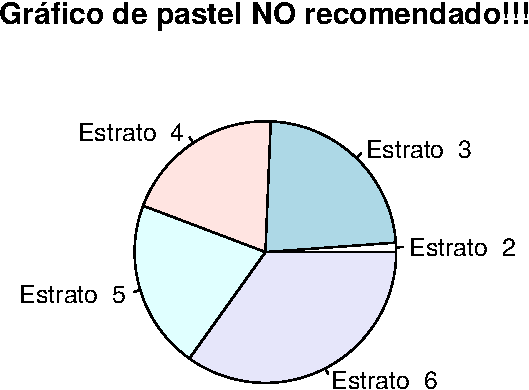
\includegraphics{Graficos_con_R_files/figure-latex/pie-1.pdf}
\caption{\label{fig:pie}Gráfico de pastel para las frecuencias relativas del
estrato socioeconómico.}
\end{figure}

La Figura \ref{fig:pie} presenta el gráfico de pastel construído con la
instrucción anterior.

\section{\texorpdfstring{Función \texttt{dotchart}
\index{gráfico de puntos}
\index{dotchart}}{Función dotchart  }}\label{funcion-dotchart}

Los gráficos de puntos son útiles para representar tablas de frecuencia
(de 1 o 2 vías) o tablas de resumen de en relación a una o dos
variables. La estructura de la función \texttt{dotchart} se muestra a
continuación.

\begin{Shaded}
\begin{Highlighting}[]
\KeywordTok{dotchart}\NormalTok{(x, }\DataTypeTok{labels=}\OtherTok{NULL}\NormalTok{, }\DataTypeTok{groups=}\OtherTok{NULL}\NormalTok{, }\DataTypeTok{gdata=}\OtherTok{NULL}\NormalTok{,}
\NormalTok{         pt.cex, pch, color, lcolor, ...)}
\end{Highlighting}
\end{Shaded}

Los argumentos de la función \texttt{dotchart} son:

\begin{itemize}
\tightlist
\item
  \texttt{x}: vector o matriz con la información de las frecuencias o
  medida de resumen a representar. Si \texttt{x} es una matriz las
  columnas representarán agrupaciones.
\item
  \texttt{labels}: vector con los nombres a usar para los puntos, por
  defecto toma los nombres de las filas de la matriz \texttt{x}.
\item
  \texttt{groups}: vector con los nombres a usar para los grupos, por
  defecto toma los nombres de las columnas de la matriz \texttt{x}.
\item
  \texttt{pt.cex}: tamaño del punto.
\item
  \texttt{pch}: tipo de punto a usar, las diferentes opciones para
  \texttt{pch} están disponibles en la Figura \ref{fig:point1}.
\item
  \texttt{color}: tipo de color usar para los puntos.
\item
  \texttt{lcolor}: color para la línea asociada a cada punto.
\item
  \texttt{...}: otros parámetros gráficos que pueden ser pasados como
  argumentos.
\end{itemize}

\subsection*{Ejemplo}\label{ejemplo-30}


Suponga que se tiene una tabla de contingencia con la información del
número de hombres y mujeres que sufren de una enfermedad rara en cuatro
ciudades importantes del mundo, a continuación la matriz \texttt{x} con
la información recolectada.

\begin{Shaded}
\begin{Highlighting}[]
\NormalTok{x <-}\StringTok{ }\KeywordTok{matrix}\NormalTok{(}\KeywordTok{c}\NormalTok{(}\DecValTok{4}\NormalTok{, }\DecValTok{6}\NormalTok{, }\DecValTok{30}\NormalTok{, }\DecValTok{18}\NormalTok{, }\DecValTok{7}\NormalTok{, }\DecValTok{13}\NormalTok{, }\DecValTok{35}\NormalTok{, }\DecValTok{20}\NormalTok{),}
            \DataTypeTok{ncol=}\DecValTok{4}\NormalTok{, }\DataTypeTok{byrow=}\OtherTok{TRUE}\NormalTok{)}
\KeywordTok{colnames}\NormalTok{(x) <-}\StringTok{ }\KeywordTok{c}\NormalTok{(}\StringTok{'Madrid'}\NormalTok{, }\StringTok{'Londres'}\NormalTok{, }\StringTok{'Paris'}\NormalTok{, }\StringTok{'Miami'}\NormalTok{)}
\KeywordTok{rownames}\NormalTok{(x) <-}\StringTok{ }\KeywordTok{c}\NormalTok{(}\StringTok{'Hombre'}\NormalTok{, }\StringTok{'Mujer'}\NormalTok{)}
\NormalTok{x}
\end{Highlighting}
\end{Shaded}

\begin{verbatim}
##        Madrid Londres Paris Miami
## Hombre      4       6    30    18
## Mujer       7      13    35    20
\end{verbatim}

En la salida anterior se presenta la matriz \texttt{x}, de esta matriz
se observa que en Madrid hay 11 personas, 4 hombres y 7 mujeres que
sufren de la enfermedad, las demás columnas se interpretan de forma
similar.

Para construir un gráfico de puntos con el objetivo de presentar la
información de la matriz \texttt{x} se utiliza el siguiente código. En
la Figura \ref{fig:dotchart2} se presenta el gráfico de puntos, de esta
figura se nota claramente que en París es donde hay más personas que
sufren de la enfermedad.

\begin{Shaded}
\begin{Highlighting}[]
\KeywordTok{dotchart}\NormalTok{(}\DataTypeTok{x=}\NormalTok{x)}
\end{Highlighting}
\end{Shaded}

\begin{figure}
\centering
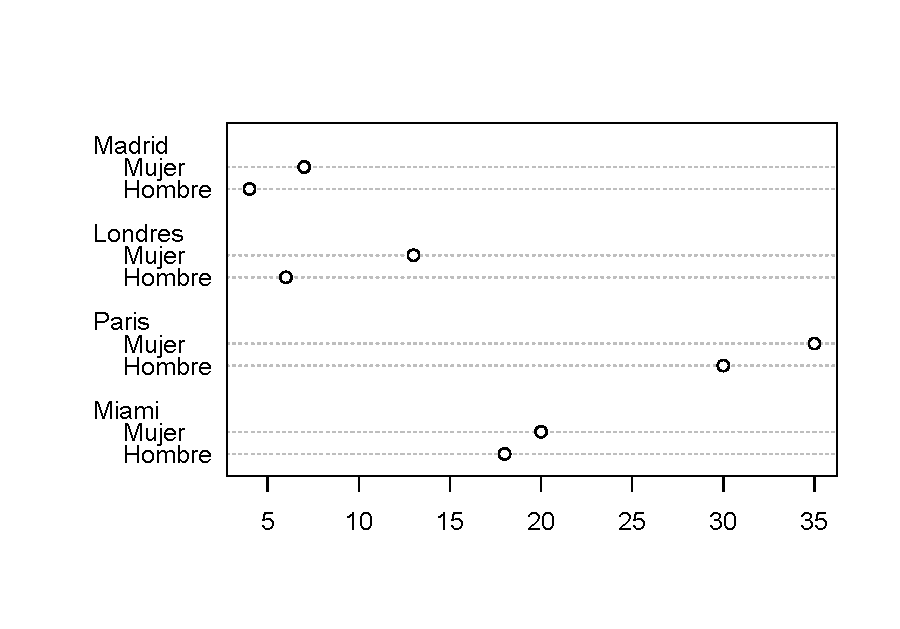
\includegraphics{Graficos_con_R_files/figure-latex/dotchart2-1.pdf}
\caption{\label{fig:dotchart2}Gráfico de puntos para una tabla de
contingencia de 2 variables.}
\end{figure}

El gráfico de puntos presentado en la Figura \ref{fig:dotchart2} se
puede mejorar usando los otros argumentos disponibles en la función
\texttt{dotchart}, a continuación el código y en la Figura
\ref{fig:dotchart3} el resultado.

\begin{Shaded}
\begin{Highlighting}[]
\KeywordTok{dotchart}\NormalTok{(}\DataTypeTok{x=}\NormalTok{x,}
         \DataTypeTok{pt.cex=}\DecValTok{2}\NormalTok{, }\DataTypeTok{pch=}\KeywordTok{c}\NormalTok{(}\DecValTok{8}\NormalTok{, }\DecValTok{21}\NormalTok{), }\DataTypeTok{color=}\KeywordTok{c}\NormalTok{(}\StringTok{'blue'}\NormalTok{, }\StringTok{'red'}\NormalTok{),}
         \DataTypeTok{lcolor=}\StringTok{'black'}\NormalTok{, }
         \DataTypeTok{xlab=}\StringTok{'Número de personas'}\NormalTok{)}
\end{Highlighting}
\end{Shaded}

\begin{figure}
\centering
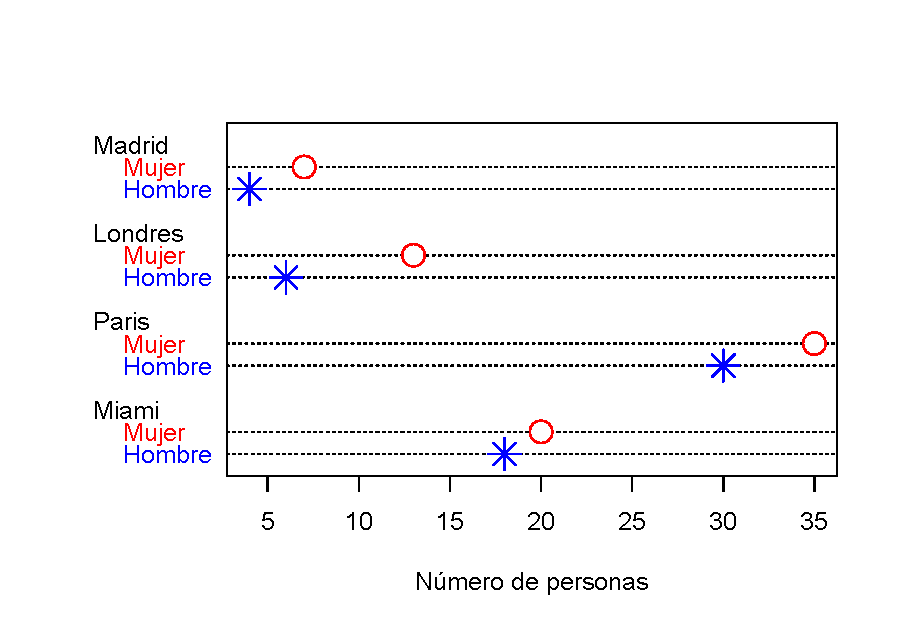
\includegraphics{Graficos_con_R_files/figure-latex/dotchart3-1.pdf}
\caption{\label{fig:dotchart3}Gráfico de puntos mejorado para una tabla de
contingencia de 2 variables.}
\end{figure}

\section*{EJERCICIOS}\label{ejercicios}


Use funciones o procedimientos (varias líneas) de \proglang{R} para
responder cada una de las siguientes preguntas.

Todas las preguntas siguientes están relacionadas con la base de datos
sobre
\href{https://raw.githubusercontent.com/fhernanb/datos/master/aptos2015}{apartamentos}
usados en la ciudad de Medellín.

\begin{enumerate}
\def\labelenumi{\arabic{enumi}.}
\tightlist
\item
  Construya un diagrama de barras para representar las frecuencias
  ABSOLUTAS de la variable ubicación.
\item
  Vuelva a construir el mismo diagrama de barras anterior pero de forma
  horizontal y agregando números de color azul para indicar las
  frecuencias.
\item
  Construya una tabla de dos vías para las variables ubicación y
  parqueadero.
\item
  Construya una tabla de frecuencias relativas para ver cómo se comporta
  la variable parqueadero dentro de cada ubicación.
\item
  Dibuje un diagrama de barras para la tabla de frecuencias del punto
  anterior.
\end{enumerate}

\chapter{\texorpdfstring{Función
\texttt{par}}{Función par}}\label{funcion-par}

En este capítulo se presentan las posibilidades que ofrece la función
\texttt{par} para la elaboración de gráficos. La función \texttt{par}
tiene 72 parámetros y a continuación se muestran.

\begin{Shaded}
\begin{Highlighting}[]
\KeywordTok{par}\NormalTok{(xlog, ylog, adj, ann, ask, bg, bty, cex, cex.axis, cex.lab,}
\NormalTok{    cex.main, cex.sub, cin, col, col.axis, col.lab, col.main,}
\NormalTok{    col.sub, cra, crt, csi, cxy, din, err, family, fg, fig, fin,}
\NormalTok{    font, font.axis, font.lab, font.main, font.sub, lab, las, }
\NormalTok{    lend, lheight, ljoin, lmitre, lty, lwd, mai, mar, mex, mfcol,}
\NormalTok{    mfg, mfrow, mgp, mkh, new, oma, omd, omi, page, pch, pin, }
\NormalTok{    plt, ps, pty, smo, srt, tck, tcl, usr, xaxp, xaxs, xaxt, xpd, }
\NormalTok{    yaxp, yaxs, yaxt, ylbias)}
\end{Highlighting}
\end{Shaded}

Para conocer los valores que tienen por defecto cada uno de estos
parámetros se puede utilizar el siguiente código.

\begin{Shaded}
\begin{Highlighting}[]
\KeywordTok{par}\NormalTok{()}
\end{Highlighting}
\end{Shaded}

Al ejecutar el código anterior se obtendrá una lista con 72 objetos en
la cual se tendrán los valores que cada uno de los parámetros asume
inicialmente en una sesión de \proglang{R}. Luego de modificar uno o
alguno de los parámetros de la función \texttt{par}, todos los gráficos
que se construyan de ahí en adelante estarán afectados por el cambio
realizado.

\BeginKnitrBlock{rmdnote}
Una buena práctica para retornar a los valores iniciales del objeto
\texttt{par()} es cerrar la ventana gráfica.
\EndKnitrBlock{rmdnote}

La utilidad de cada uno de los parámetros para personalizar los gráficos
se mostrará por medio de ejemplos.

\section{\texorpdfstring{Parámetro \texttt{ann}
\index{nombre de los ejes}
\index{ann}}{Parámetro ann  }}\label{parametro-ann}

Este parámetro sirve para indicar si se quiere un gráfico con nombres en
los ejes y título principal, por defecto asume el valor \texttt{TRUE}.

\subsection*{Ejemplo}\label{ejemplo-31}


Dibujar la densidad para una distribución \(\chi^2_1\) usando
\texttt{ann=FALSE} dentro de la función \texttt{par}.

El código necesario para obtener la figura se muestra a continuación.
Note que a pesar de haber solicitado título principal y nombres de los
ejes, éstos no aparecen en el resultado final porque se usó antes
\texttt{par(ann=FALSE)}. En la Figura \ref{fig:ann} se muestra el
gráfico solicitado.

\begin{Shaded}
\begin{Highlighting}[]
\KeywordTok{par}\NormalTok{(}\DataTypeTok{ann=}\OtherTok{FALSE}\NormalTok{)}
\KeywordTok{curve}\NormalTok{(}\KeywordTok{dchisq}\NormalTok{(x, }\DataTypeTok{df=}\DecValTok{1}\NormalTok{), }\DataTypeTok{col=}\StringTok{'salmon1'}\NormalTok{, }\DataTypeTok{lwd=}\DecValTok{4}\NormalTok{,}
      \DataTypeTok{main=}\StringTok{'Chi cuadrada'}\NormalTok{,}
      \DataTypeTok{xlab=}\StringTok{'x'}\NormalTok{, }\DataTypeTok{ylab=}\StringTok{'Densidad'}\NormalTok{)}
\end{Highlighting}
\end{Shaded}

\begin{figure}
\centering
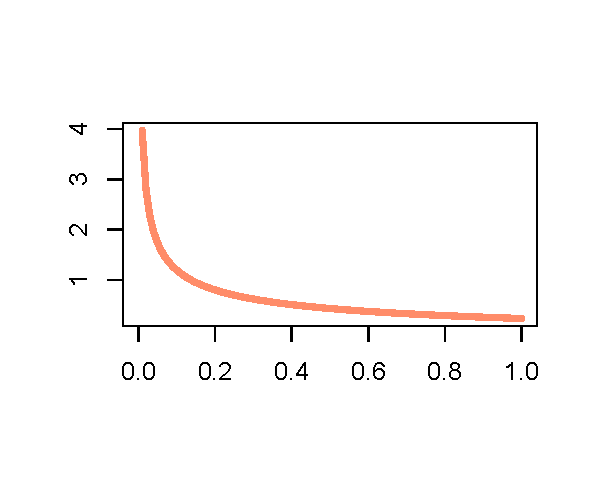
\includegraphics{Graficos_con_R_files/figure-latex/ann-1.pdf}
\caption{\label{fig:ann}Efecto del parámetro \texttt{ann}.}
\end{figure}

\BeginKnitrBlock{rmdnote}
La opción \texttt{ann=FALSE} es muy útil para gráficos sin nombres en
los ejes y sin título principal. Esta opción evita el uso de
\texttt{xlab=\textquotesingle{}\textquotesingle{},\ ylab=\textquotesingle{}\textquotesingle{},\ main=\textquotesingle{}\textquotesingle{}}
dentro de las funciones gráficas.
\EndKnitrBlock{rmdnote}

\section{\texorpdfstring{Parámetro \texttt{adj}
\index{justitificación del texto}
\index{adj}}{Parámetro adj  }}\label{parametro-adj}

Este parámetro sirve para modificar la justificación del texto cuando se
usan las funciones \texttt{text}, \texttt{mtext} y \texttt{title}. Su
valor por defecto es 0.5 que indica que el texto debe quedar centrado en
las coordenadas x e y indicadas, un valor de 0 significa justificación a
izquierda mientras que 1 significa justificación a derecha.

\subsection*{Ejemplo}\label{ejemplo-32}


Dibujar un gráfico vacío, ubicar las palabra \emph{hola mi mundo}
horizontalmente en el gráfico y explorar el efecto del parámetro
\texttt{adj}.

El código necesario para obtener lo solicitado se muestra a
continuación. Se agregaron líneas a trazos de color azul para indicar el
sitio exacto donde se quería el texto. Observando la Figura
\ref{fig:adj} se nota claramente que cuando \texttt{adj=0.5} la palabra
queda centrada mientras que con otros valores cambia la justificación
del texto.

\begin{Shaded}
\begin{Highlighting}[]
\KeywordTok{plot}\NormalTok{(}\OtherTok{NULL}\NormalTok{, }\DataTypeTok{xlim=}\KeywordTok{c}\NormalTok{(}\DecValTok{0}\NormalTok{, }\FloatTok{0.6}\NormalTok{), }\DataTypeTok{ylim=}\KeywordTok{c}\NormalTok{(}\DecValTok{0}\NormalTok{, }\DecValTok{1}\NormalTok{))}

\KeywordTok{par}\NormalTok{(}\DataTypeTok{adj=}\DecValTok{0}\NormalTok{)  }\CommentTok{# Para justificar a izquierda}
\KeywordTok{text}\NormalTok{(}\DataTypeTok{x=}\FloatTok{0.1}\NormalTok{, }\DataTypeTok{y=}\FloatTok{0.6}\NormalTok{, }\StringTok{'hola'}\NormalTok{, }\DataTypeTok{cex=}\DecValTok{3}\NormalTok{)}

\KeywordTok{par}\NormalTok{(}\DataTypeTok{adj=}\FloatTok{0.5}\NormalTok{)  }\CommentTok{# Para justificar centrado}
\KeywordTok{text}\NormalTok{(}\DataTypeTok{x=}\FloatTok{0.3}\NormalTok{, }\DataTypeTok{y=}\FloatTok{0.6}\NormalTok{, }\StringTok{'mi'}\NormalTok{, }\DataTypeTok{cex=}\DecValTok{3}\NormalTok{)}

\KeywordTok{par}\NormalTok{(}\DataTypeTok{adj=}\DecValTok{1}\NormalTok{)  }\CommentTok{# Para justificar a derecha}
\KeywordTok{text}\NormalTok{(}\DataTypeTok{x=}\FloatTok{0.5}\NormalTok{, }\DataTypeTok{y=}\FloatTok{0.6}\NormalTok{, }\StringTok{'mundo'}\NormalTok{, }\DataTypeTok{cex=}\DecValTok{3}\NormalTok{)}

\KeywordTok{abline}\NormalTok{(}\DataTypeTok{h=}\FloatTok{0.6}\NormalTok{, }\DataTypeTok{v=}\KeywordTok{c}\NormalTok{(}\FloatTok{0.1}\NormalTok{, }\FloatTok{0.3}\NormalTok{, }\FloatTok{0.5}\NormalTok{),}
       \DataTypeTok{lty=}\DecValTok{3}\NormalTok{, }\DataTypeTok{col=}\StringTok{'deepskyblue3'}\NormalTok{)}
\end{Highlighting}
\end{Shaded}

\begin{figure}
\centering
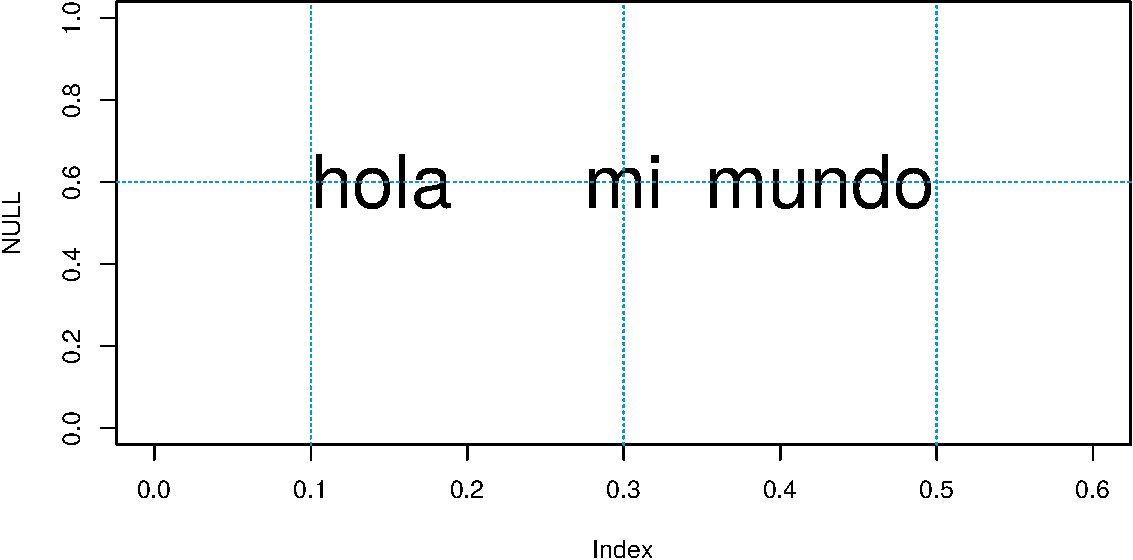
\includegraphics{Graficos_con_R_files/figure-latex/adj-1.pdf}
\caption{\label{fig:adj}Efecto del parámetro \texttt{adj}.}
\end{figure}

\section{\texorpdfstring{Parámetro \texttt{bg} \index{color del fondo}
\index{bg}}{Parámetro bg  }}\label{parametro-bg}

Este parámetro sirve para modificar el color del fondo donde se va a
dibujar.

\subsection*{Ejemplo}\label{ejemplo-33}


Dibujar la densidad de una normal estándar usando un color verde para el
fondo.

A continuación el código necesario para modficar el color del fondo. En
esta
\href{http://www.stat.columbia.edu/~tzheng/files/Rcolor.pdf}{página} se
puede encontrar una paleta de colores disponibles en \proglang{R}. En la
Figura \ref{fig:bg} se muestra el resultado, el color de fondo está por
toda la ventana gráfica.

\begin{Shaded}
\begin{Highlighting}[]
\KeywordTok{par}\NormalTok{(}\DataTypeTok{bg=}\StringTok{'darkseagreen1'}\NormalTok{)}
\KeywordTok{curve}\NormalTok{(dnorm, }\DataTypeTok{lwd=}\DecValTok{6}\NormalTok{, }\DataTypeTok{col=}\StringTok{'blue'}\NormalTok{, }\DataTypeTok{xlim=}\KeywordTok{c}\NormalTok{(}\OperatorTok{-}\DecValTok{4}\NormalTok{, }\DecValTok{4}\NormalTok{))}
\end{Highlighting}
\end{Shaded}

\begin{figure}
\centering
\includegraphics{Graficos_con_R_files/figure-latex/bg-1.pdf}
\caption{\label{fig:bg}Efecto del parámetro \texttt{bg}.}
\end{figure}

\section{\texorpdfstring{Parámetro \texttt{mfrow}
\index{partición ventana gráfica}
\index{mfrow}}{Parámetro mfrow  }}\label{parametro-mfrow}

Este parámetro sirve para dividir la ventana gráfica en forma de matriz
para almacenar en cada celda un gráfico diferente. La forma para
modificar este parámetro es \texttt{mfrow=c(nf,\ nc)}, donde \texttt{nf}
es el número de filas y \texttt{nc} el número de columnas en las cuales
se va a dividir la ventana gráfica.

\subsection*{Ejemplo}\label{ejemplo-34}


Dibujar la distribución de probabilidad para una distribución Poisson
con \(\lambda=1, 3, 7, 15\).

Note que el objetivo es repetir el mismo gráfico para 4 valores
diferentes del paramétro \(\lambda\), por lo tanto se escribirá una sola
vez el código de interés pero se repetirá automáticamente 4 veces para
cada valor de \(\lambda\). Para construir el gráfico solicitado
iniciamos partiendo la ventana gráfica en una matriz de \(2 \times 2\)
usando \texttt{par(mfrow=c(2,\ 2))}. Luego se construye el vector
\texttt{lambdas} con los valores de \(\lambda\) y por último se coloca
el \texttt{plot} de interés dentro de una sentencia \texttt{for}. Abajo
el código utilizado.

\begin{Shaded}
\begin{Highlighting}[]
\KeywordTok{par}\NormalTok{(}\DataTypeTok{mfrow=}\KeywordTok{c}\NormalTok{(}\DecValTok{2}\NormalTok{, }\DecValTok{2}\NormalTok{))}

\NormalTok{lambdas <-}\StringTok{ }\KeywordTok{c}\NormalTok{(}\DecValTok{1}\NormalTok{, }\DecValTok{3}\NormalTok{, }\DecValTok{7}\NormalTok{, }\DecValTok{15}\NormalTok{)}

\ControlFlowTok{for}\NormalTok{ (i }\ControlFlowTok{in} \DecValTok{1}\OperatorTok{:}\DecValTok{4}\NormalTok{) \{}
  \KeywordTok{plot}\NormalTok{(}\KeywordTok{dpois}\NormalTok{(}\DataTypeTok{x=}\DecValTok{0}\OperatorTok{:}\DecValTok{30}\NormalTok{, }\DataTypeTok{lambda=}\NormalTok{lambdas[i]), }\DataTypeTok{lwd=}\DecValTok{4}\NormalTok{,}
       \DataTypeTok{type=}\StringTok{'h'}\NormalTok{, }\DataTypeTok{xlab=}\StringTok{'x'}\NormalTok{, }\DataTypeTok{ylab=}\StringTok{'Probabilidad'}\NormalTok{)}
  \KeywordTok{title}\NormalTok{(}\KeywordTok{bquote}\NormalTok{(}\OperatorTok{~}\StringTok{ }\NormalTok{lambda }\OperatorTok{==}\StringTok{ }\NormalTok{.(lambdas[i])))}
\NormalTok{\} }
\end{Highlighting}
\end{Shaded}

\begin{figure}
\centering
\includegraphics{Graficos_con_R_files/figure-latex/mfrow-1.pdf}
\caption{\label{fig:mfrow}Efecto del parámetro \texttt{mfrow}.}
\end{figure}

En la Figura \ref{fig:mfrow} se muestra la distribución de probabilidad
para cada uno de los 4 valores de \(\lambda\) en la misma figura.

\BeginKnitrBlock{rmdnote}
La función \texttt{bquote} sirve para construir mensajes que sean una
mezcla de texto, expresiones matemáticas y valores de un objeto.
\EndKnitrBlock{rmdnote}

\section{\texorpdfstring{Parámetro \texttt{bty} \index{tipo de caja}
\index{bty}}{Parámetro bty  }}\label{parametro-bty}

Este parámetro sirve para modficar la caja alrededor del gráfico
construído. Los posibles valores para este parámetro son:
\texttt{\textquotesingle{}o\textquotesingle{}} valor por defecto para
obtener la caja usual; se pueden usar también los símboloes
\texttt{\textquotesingle{}l\textquotesingle{}},
\texttt{\textquotesingle{}7\textquotesingle{}},
\texttt{\textquotesingle{}c\textquotesingle{}},
\texttt{\textquotesingle{}u\textquotesingle{}} o
\texttt{\textquotesingle{}{]}\textquotesingle{}}, el resultado será una
caja con la forma del símbolo; se puede usar
\texttt{\textquotesingle{}n\textquotesingle{}} para suprimir la caja.

\subsection*{Ejemplo}\label{ejemplo-35}


Dibujar la densidad de una \(\chi^2_5\) modificando el parámetro
\texttt{bty} de \texttt{par}.

A continuación el código para dibujar la misma densidad 4 veces
modificando el valor para \texttt{bty}. En la Figura \ref{fig:par2} se
muestra el efecto que tienen los valores elegidos. Observe que, además
de los ejes, hay una caja cuya forma depende el valor seleccionado,
cuando \texttt{bty=\textquotesingle{}u\textquotesingle{}} el resultado
es una caja con esa misma forma.

\begin{Shaded}
\begin{Highlighting}[]
\KeywordTok{par}\NormalTok{(}\DataTypeTok{bty=}\StringTok{'n'}\NormalTok{, }\DataTypeTok{mfrow=}\KeywordTok{c}\NormalTok{(}\DecValTok{2}\NormalTok{, }\DecValTok{2}\NormalTok{))}
\KeywordTok{curve}\NormalTok{(}\KeywordTok{dchisq}\NormalTok{(x, }\DataTypeTok{df=}\DecValTok{5}\NormalTok{), }\DataTypeTok{xlim=}\KeywordTok{c}\NormalTok{(}\DecValTok{0}\NormalTok{, }\DecValTok{20}\NormalTok{))}
\KeywordTok{title}\NormalTok{(}\StringTok{"Usando bty='n'"}\NormalTok{)}
\KeywordTok{par}\NormalTok{(}\DataTypeTok{bty=}\StringTok{'o'}\NormalTok{)}
\KeywordTok{curve}\NormalTok{(}\KeywordTok{dchisq}\NormalTok{(x, }\DataTypeTok{df=}\DecValTok{5}\NormalTok{), }\DataTypeTok{xlim=}\KeywordTok{c}\NormalTok{(}\DecValTok{0}\NormalTok{, }\DecValTok{20}\NormalTok{))}
\KeywordTok{title}\NormalTok{(}\StringTok{"Usando bty='o'"}\NormalTok{)}
\KeywordTok{par}\NormalTok{(}\DataTypeTok{bty=}\StringTok{'u'}\NormalTok{)}
\KeywordTok{curve}\NormalTok{(}\KeywordTok{dchisq}\NormalTok{(x, }\DataTypeTok{df=}\DecValTok{5}\NormalTok{), }\DataTypeTok{xlim=}\KeywordTok{c}\NormalTok{(}\DecValTok{0}\NormalTok{, }\DecValTok{20}\NormalTok{))}
\KeywordTok{title}\NormalTok{(}\StringTok{"Usando bty='u'"}\NormalTok{)}
\KeywordTok{par}\NormalTok{(}\DataTypeTok{bty=}\StringTok{'l'}\NormalTok{)}
\KeywordTok{curve}\NormalTok{(}\KeywordTok{dchisq}\NormalTok{(x, }\DataTypeTok{df=}\DecValTok{5}\NormalTok{), }\DataTypeTok{xlim=}\KeywordTok{c}\NormalTok{(}\DecValTok{0}\NormalTok{, }\DecValTok{20}\NormalTok{))}
\KeywordTok{title}\NormalTok{(}\StringTok{"Usando bty='l'"}\NormalTok{)}
\end{Highlighting}
\end{Shaded}

\begin{figure}
\centering
\includegraphics{Graficos_con_R_files/figure-latex/par2-1.pdf}
\caption{\label{fig:par2}Efecto del parámetro \texttt{bty}.}
\end{figure}

\section{\texorpdfstring{Parámetro \texttt{cex}
\index{tamaño de símbolos}
\index{cex}}{Parámetro cex  }}\label{parametro-cex}

Este parámetro sirve para modificar el tamaño de los símbolos, nombres
de los ejes, marcas de los ejes y títulos. El valor por defecto es
\texttt{cex=1}, valores mayores a uno generan gráficos con símbolos,
títulos y marcas grandes, incluso desproporcionados; valores pequeños de
este parámetro permiten obtener mejores figuras. A continuación un
ejemplo para ver el efecto que tiene este parámetro sobre las figuras
obtenidas.

\subsection*{Ejemplo}\label{ejemplo-36}


Hacer un gráfico de dispersión sencillo para explorar el efecto del
parámetro \texttt{cex}.

Se construirá un gráfico de dispersión dos veces, en la primera con
parámetro \texttt{cex=1} y en la segunda ocasión usando
\texttt{cex=0.6}. Abajo el código utilizado. En el pánel izquierdo de la
Figura \ref{fig:cex} está el diagrama de dispersión obtenido con
\texttt{cex=1.4} mientras que el de la derecha fue obtenido con
\texttt{cex=0.6}. Observe cómo se modificaron los nombres de los ejes,
título principal, marcas de los ejes y tamaño del símbolo.

\begin{Shaded}
\begin{Highlighting}[]
\NormalTok{x <-}\StringTok{ }\OperatorTok{-}\DecValTok{3}\OperatorTok{:}\DecValTok{3}
\KeywordTok{par}\NormalTok{(}\DataTypeTok{mfrow=}\KeywordTok{c}\NormalTok{(}\DecValTok{1}\NormalTok{, }\DecValTok{2}\NormalTok{), }\DataTypeTok{cex=}\FloatTok{1.4}\NormalTok{)}
\KeywordTok{plot}\NormalTok{(}\DataTypeTok{x=}\NormalTok{x, }\DataTypeTok{y=}\NormalTok{x, }\DataTypeTok{main=}\StringTok{'Usando }\CharTok{\textbackslash{}n}\StringTok{ cex=1.4'}\NormalTok{)}

\KeywordTok{par}\NormalTok{(}\DataTypeTok{cex=}\FloatTok{0.6}\NormalTok{)}
\KeywordTok{plot}\NormalTok{(}\DataTypeTok{x=}\NormalTok{x, }\DataTypeTok{y=}\NormalTok{x, }\DataTypeTok{main=}\StringTok{'Usando }\CharTok{\textbackslash{}n}\StringTok{ cex=0.6'}\NormalTok{)}
\end{Highlighting}
\end{Shaded}

\begin{figure}
\centering
\includegraphics{Graficos_con_R_files/figure-latex/cex-1.pdf}
\caption{\label{fig:cex}Efecto del parámetro \texttt{cex}.}
\end{figure}

El parámetro \texttt{cex} tiene un efecto importante en las figuras, se
recomienda al usuario que cada vez que construya una figura explore
diferentes opciones para obtener una figura que exprese la esencia de lo
que desea comunicar.

\section{\texorpdfstring{Parámetros \texttt{cex.axis}, \texttt{cex.lab},
\texttt{cex.main} y \texttt{cex.sub} \index{cex.axis} \index{cex.lab}
\index{cex.main}
\index{cex.sub}}{Parámetros cex.axis, cex.lab, cex.main y cex.sub    }}\label{parametros-cex.axis-cex.lab-cex.main-y-cex.sub}

Los parámetros \texttt{cex.axis}, \texttt{cex.lab}, \texttt{cex.main} y
\texttt{cex.sub} sirven para modificar el tamaño de las marcas en los
ejes, el tamaño de los nombres de los ejes, el tamaño del título
principal y el tamaño del subtítulo respectivamente. El parámetro
\texttt{cex} explicado en la sección anterior, modifica el tamaño de los
anteriores elementos simultáneamente mientras que los parámetros
explicados en esta sección modifican cada uno de los elementos por
aparte.

\subsection*{Ejemplo}\label{ejemplo-37}


Hacer un gráfico cualquiera y modificar los parámetros
\texttt{cex.axis}, \texttt{cex.lab}, \texttt{cex.main} y
\texttt{cex.sub} de la función \texttt{par} con el objetivo de ver el
efecto que ellos tiene sobre el gráfico.

A continuación se construye un gráfico simple y se modifican todos los
paramétros \texttt{cex.algo} para ver el efecto que ellos tienen sobre
el gráfico resultante, abajo el código usado.

En la Figura \ref{fig:cexs} se muestra el resultado. Observe que las
marcas y números en los ejes quedaron grandes debido a que se usó
\texttt{cex.axis=1.8}, los nombres que identifican los ejes casi no se
ven porque se usó \texttt{cex.lab=0.3}. El título principal quedó muy
pequeño debido a que \texttt{cex.main=0.7} mientras que el subtítulo
quedó demasiado grande porque se usó \texttt{cex.sub=2}. Este ejemplo
muestra que el usuario tiene todo el control para construir gráficos
personalizados en \proglang{R}.

\begin{Shaded}
\begin{Highlighting}[]
\NormalTok{x <-}\StringTok{ }\OperatorTok{-}\DecValTok{3}\OperatorTok{:}\DecValTok{3}
\KeywordTok{par}\NormalTok{(}\DataTypeTok{cex.axis=}\FloatTok{1.8}\NormalTok{, }\DataTypeTok{cex.lab=}\FloatTok{0.3}\NormalTok{, }\DataTypeTok{cex.main=}\FloatTok{0.7}\NormalTok{, }\DataTypeTok{cex.sub=}\FloatTok{2.0}\NormalTok{)}
\KeywordTok{plot}\NormalTok{(}\DataTypeTok{x=}\NormalTok{x, }\DataTypeTok{y=}\NormalTok{x,}
     \DataTypeTok{xlab=}\StringTok{'Valores de x'}\NormalTok{, }\DataTypeTok{ylab=}\StringTok{'Valores de y'}\NormalTok{,}
     \DataTypeTok{main=}\StringTok{'Título principal'}\NormalTok{,}
     \DataTypeTok{sub=}\StringTok{'Subtítulo'}\NormalTok{)}
\end{Highlighting}
\end{Shaded}

\begin{figure}
\centering
\includegraphics{Graficos_con_R_files/figure-latex/cexs-1.pdf}
\caption{\label{fig:cexs}Efecto de los parámetros \texttt{cex.axis},
\texttt{cex.lab}, \texttt{cex.main} y \texttt{cex.sub}.}
\end{figure}

\section{\texorpdfstring{Parámetro \texttt{col}, \texttt{col.axis},
\texttt{col.lab}, \texttt{col.main} y \texttt{col.sub} \index{color}
\index{col}}{Parámetro col, col.axis, col.lab, col.main y col.sub  }}\label{parametro-col-col.axis-col.lab-col.main-y-col.sub}

Estos parámetros sirven para definir el color a usar en los ejes, en los
nombres de los ejes, en el título y en el subtítulo.

\subsection*{Ejemplo}\label{ejemplo-38}


Hacer un gráfico cualquiera y modificar los parámetros \texttt{col},
\texttt{col.axis}, \texttt{col.lab}, \texttt{col.main} y
\texttt{col.sub} de la función \texttt{par} con el objetivo de ver el
efecto que ellos tiene sobre el gráfico.

A continuación se construye un gráfico simple y se modifican todos los
paramétros para ver el efecto que ellos tienen sobre el gráfico
resultante, abajo el código usado.

\begin{Shaded}
\begin{Highlighting}[]
\KeywordTok{par}\NormalTok{(}\DataTypeTok{col=}\StringTok{'blue'}\NormalTok{, }\DataTypeTok{col.axis=}\StringTok{'red'}\NormalTok{, }\DataTypeTok{col.lab=}\StringTok{'orange'}\NormalTok{,}
    \DataTypeTok{col.main=}\StringTok{'darkgreen'}\NormalTok{, }\DataTypeTok{col.sub=}\StringTok{'purple'}\NormalTok{, }\DataTypeTok{bty=}\StringTok{'n'}\NormalTok{)}
\KeywordTok{plot}\NormalTok{(}\DecValTok{1}\OperatorTok{:}\DecValTok{10}\NormalTok{, }\DataTypeTok{pch=}\DecValTok{20}\NormalTok{, }\DataTypeTok{cex=}\DecValTok{2}\NormalTok{, }\DataTypeTok{las=}\DecValTok{1}\NormalTok{,}
     \DataTypeTok{main=}\StringTok{'Título'}\NormalTok{, }\DataTypeTok{xlab=}\StringTok{'Nombre eje X'}\NormalTok{,}
     \DataTypeTok{ylab=}\StringTok{'Nombre eje Y'}\NormalTok{, }\DataTypeTok{sub=}\StringTok{'Subtítulo'}\NormalTok{)}
\end{Highlighting}
\end{Shaded}

\begin{figure}
\centering
\includegraphics{Graficos_con_R_files/figure-latex/cols-1.pdf}
\caption{\label{fig:cols}Efecto de los parámetros \texttt{col},
\texttt{col.axis}, \texttt{col.lab}, \texttt{col.main} y
\texttt{col.sub}.}
\end{figure}

En la Figura \ref{fig:cols} se muestra el efecto de los parámetros
\texttt{col}, \texttt{col.axis}, \texttt{col.lab}, \texttt{col.main} y
\texttt{col.sub} de la función \texttt{par}.

\chapter{Funciones auxiliares}\label{funciones-auxiliares}

En este capítulo se presentan funciones auxiliares que son útiles para
complementar los gráficos generados en \proglang{R}.

\section{\texorpdfstring{Función \texttt{segments} \index{segments}
\index{segmentos}}{Función segments  }}\label{funcion-segments}

Esta función es muy útil para digujar segmentos. La estructura de la
función se muestra a continuación.

\begin{Shaded}
\begin{Highlighting}[]
\KeywordTok{segments}\NormalTok{(x0, y0, }\DataTypeTok{x1 =}\NormalTok{ x0, }\DataTypeTok{y1 =}\NormalTok{ y0, ...)}
\end{Highlighting}
\end{Shaded}

Los argumentos de la función son:

\begin{itemize}
\tightlist
\item
  \texttt{xo,\ yo}: coordenadas del punto de inicio del segmento.
\item
  \texttt{x1,\ y1}: coordenadas del punto de fin del segmento.
\item
  \texttt{...}: otros parámetros gráficos.
\end{itemize}

A continuación de muestra el código para dibujar con segmentos la sigla
de la Universidad Nacional de Colombia (UN), en la Figura \ref{fig:seg1}
se puede ver el resultado.

\begin{Shaded}
\begin{Highlighting}[]
\KeywordTok{plot}\NormalTok{(}\KeywordTok{c}\NormalTok{(}\OperatorTok{-}\DecValTok{11}\NormalTok{, }\DecValTok{3}\NormalTok{), }\KeywordTok{c}\NormalTok{(}\OperatorTok{-}\DecValTok{10}\NormalTok{, }\DecValTok{10}\NormalTok{), }\DataTypeTok{type=}\StringTok{"n"}\NormalTok{, }\DataTypeTok{xlab=}\StringTok{""}\NormalTok{, }\DataTypeTok{ylab=}\StringTok{""}\NormalTok{)}
\KeywordTok{grid}\NormalTok{()}

\KeywordTok{segments}\NormalTok{(}\OperatorTok{-}\DecValTok{9}\NormalTok{, }\DecValTok{9}\NormalTok{, }\OperatorTok{-}\DecValTok{9}\NormalTok{, }\OperatorTok{-}\DecValTok{9}\NormalTok{, }\DataTypeTok{lwd=}\DecValTok{4}\NormalTok{, }\DataTypeTok{col=}\DecValTok{3}\NormalTok{)}
\KeywordTok{segments}\NormalTok{(}\OperatorTok{-}\DecValTok{9}\NormalTok{, }\OperatorTok{-}\DecValTok{9}\NormalTok{, }\OperatorTok{-}\DecValTok{5}\NormalTok{, }\OperatorTok{-}\DecValTok{9}\NormalTok{, }\DataTypeTok{lwd=}\DecValTok{4}\NormalTok{, }\DataTypeTok{col=}\DecValTok{3}\NormalTok{)}
\KeywordTok{segments}\NormalTok{(}\OperatorTok{-}\DecValTok{5}\NormalTok{, }\OperatorTok{-}\DecValTok{9}\NormalTok{, }\OperatorTok{-}\DecValTok{5}\NormalTok{, }\DecValTok{9}\NormalTok{, }\DataTypeTok{lwd=}\DecValTok{4}\NormalTok{, }\DataTypeTok{col=}\DecValTok{3}\NormalTok{)}

\KeywordTok{segments}\NormalTok{(}\OperatorTok{-}\DecValTok{4}\NormalTok{, }\OperatorTok{-}\DecValTok{9}\NormalTok{, }\OperatorTok{-}\DecValTok{4}\NormalTok{, }\DecValTok{9}\NormalTok{, }\DataTypeTok{lwd=}\DecValTok{4}\NormalTok{)}
\KeywordTok{segments}\NormalTok{(}\OperatorTok{-}\DecValTok{4}\NormalTok{, }\DecValTok{9}\NormalTok{, }\DecValTok{0}\NormalTok{, }\OperatorTok{-}\DecValTok{9}\NormalTok{, }\DataTypeTok{lwd=}\DecValTok{4}\NormalTok{)}
\KeywordTok{segments}\NormalTok{(}\DecValTok{0}\NormalTok{, }\OperatorTok{-}\DecValTok{9}\NormalTok{, }\DecValTok{0}\NormalTok{, }\DecValTok{9}\NormalTok{, }\DataTypeTok{lwd=}\DecValTok{4}\NormalTok{)}
\end{Highlighting}
\end{Shaded}

\begin{figure}
\centering
\includegraphics{Graficos_con_R_files/figure-latex/seg1-1.pdf}
\caption{\label{fig:seg1}Ejemplos de segmentos.}
\end{figure}

\section{\texorpdfstring{Función \texttt{rect} \index{rect}
\index{rectángulos}}{Función rect  }}\label{funcion-rect}

Esta función es muy útil para digujar rectángulos. La estructura de la
función se muestra a continuación.

\begin{Shaded}
\begin{Highlighting}[]
\KeywordTok{rect}\NormalTok{(xleft, ybottom, xright, ytop,}
     \DataTypeTok{density =} \OtherTok{NULL}\NormalTok{, }\DataTypeTok{angle =} \DecValTok{45}\NormalTok{, ...)}
\end{Highlighting}
\end{Shaded}

Los argumentos de la función son:

\begin{itemize}
\tightlist
\item
  \texttt{xleft}: vector o escalar con la posición de x a izquierda.
\item
  \texttt{ybottom}: vector o escalar con la posición de y abajo.
\item
  \texttt{xright}: vector o escalar con la posición de x a derecha.
\item
  \texttt{ytop}: vector o escalar con la posición de y arriba.
\item
  \texttt{density}: número de líneas por pulgada con la cuales se
  rellenará el rectángulo.
\item
  \texttt{angle}: ángulo de inclinación de la líneas de relleno.
\item
  \texttt{col}: color para el fondo del rectángulo.
\item
  \texttt{border}: color para el borde del rectángulo, un valor posible
  es \texttt{\textquotesingle{}transparent\textquotesingle{}} cuando no
  se desea borde.
\item
  \texttt{...}: otros parámetros gráficos.
\end{itemize}

En la Figura \ref{fig:rect1} se muestran 7 rectángulos de ejemplo que
fueron obtenidos al variar los parámetros de la función \texttt{rect}, a
continuación el código usado para obtener esa figura.

\begin{Shaded}
\begin{Highlighting}[]
\KeywordTok{plot}\NormalTok{(}\OtherTok{NA}\NormalTok{, }\DataTypeTok{xlim=}\KeywordTok{c}\NormalTok{(}\DecValTok{10}\NormalTok{, }\DecValTok{20}\NormalTok{), }\DataTypeTok{ylim=}\KeywordTok{c}\NormalTok{(}\DecValTok{10}\NormalTok{, }\DecValTok{30}\NormalTok{), }\DataTypeTok{las=}\DecValTok{1}\NormalTok{, }\DataTypeTok{xlab=}\StringTok{''}\NormalTok{, }\DataTypeTok{ylab=}\StringTok{''}\NormalTok{)}
\KeywordTok{rect}\NormalTok{(}\DecValTok{10}\NormalTok{, }\DecValTok{28}\NormalTok{, }\DecValTok{12}\NormalTok{, }\DecValTok{30}\NormalTok{)}
\KeywordTok{rect}\NormalTok{(}\DecValTok{11}\NormalTok{, }\DecValTok{25}\NormalTok{, }\DecValTok{13}\NormalTok{, }\DecValTok{27}\NormalTok{, }\DataTypeTok{col=}\StringTok{'red'}\NormalTok{)}
\KeywordTok{rect}\NormalTok{(}\DecValTok{12}\NormalTok{, }\DecValTok{22}\NormalTok{, }\DecValTok{14}\NormalTok{, }\DecValTok{24}\NormalTok{, }\DataTypeTok{density=}\DecValTok{5}\NormalTok{)}
\KeywordTok{rect}\NormalTok{(}\DecValTok{13}\NormalTok{, }\DecValTok{19}\NormalTok{, }\DecValTok{15}\NormalTok{, }\DecValTok{21}\NormalTok{, }\DataTypeTok{density=}\DecValTok{5}\NormalTok{, }\DataTypeTok{angle=}\DecValTok{15}\NormalTok{)}
\KeywordTok{rect}\NormalTok{(}\DecValTok{14}\NormalTok{, }\DecValTok{16}\NormalTok{, }\DecValTok{16}\NormalTok{, }\DecValTok{18}\NormalTok{, }\DataTypeTok{col=}\StringTok{'pink'}\NormalTok{, }\DataTypeTok{border=}\StringTok{'blue'}\NormalTok{)}
\KeywordTok{rect}\NormalTok{(}\DecValTok{15}\NormalTok{, }\DecValTok{13}\NormalTok{, }\DecValTok{17}\NormalTok{, }\DecValTok{15}\NormalTok{, }\DataTypeTok{lty=}\StringTok{'dashed'}\NormalTok{)}
\KeywordTok{rect}\NormalTok{(}\DecValTok{16}\NormalTok{, }\DecValTok{10}\NormalTok{, }\DecValTok{18}\NormalTok{, }\DecValTok{12}\NormalTok{, }\DataTypeTok{lwd=}\DecValTok{3}\NormalTok{)}

\KeywordTok{text}\NormalTok{(}\DecValTok{14}\NormalTok{, }\DecValTok{26}\NormalTok{, }\StringTok{"col='red'"}\NormalTok{)}
\KeywordTok{text}\NormalTok{(}\DecValTok{15}\NormalTok{, }\DecValTok{23}\NormalTok{, }\StringTok{"density=5"}\NormalTok{)}
\KeywordTok{text}\NormalTok{(}\DecValTok{17}\NormalTok{, }\DecValTok{20}\NormalTok{, }\StringTok{"density=5, angle=15"}\NormalTok{)}
\KeywordTok{text}\NormalTok{(}\FloatTok{18.2}\NormalTok{, }\DecValTok{17}\NormalTok{, }\StringTok{"col='pink', border='blue'"}\NormalTok{)}
\KeywordTok{text}\NormalTok{(}\FloatTok{18.2}\NormalTok{, }\DecValTok{14}\NormalTok{, }\StringTok{"lty='dashed'"}\NormalTok{)}
\KeywordTok{text}\NormalTok{(}\FloatTok{18.8}\NormalTok{, }\DecValTok{11}\NormalTok{, }\StringTok{"lwd=3"}\NormalTok{)}
\end{Highlighting}
\end{Shaded}

\begin{figure}
\centering
\includegraphics{Graficos_con_R_files/figure-latex/rect1-1.pdf}
\caption{\label{fig:rect1}Ejemplos de rectángulos.}
\end{figure}

El código mostrado abajo pertenece a la ayuda de la función
\texttt{rect} y el resultado es la Figura \ref{fig:rect2}. De esta
figura se observa que es posible dibujar varios rectángulos ingresando
las coordenadas como vectores.

\begin{Shaded}
\begin{Highlighting}[]
\NormalTok{## set up the plot region:}
\KeywordTok{plot}\NormalTok{(}\KeywordTok{c}\NormalTok{(}\DecValTok{100}\NormalTok{, }\DecValTok{250}\NormalTok{), }\KeywordTok{c}\NormalTok{(}\DecValTok{300}\NormalTok{, }\DecValTok{450}\NormalTok{), }\DataTypeTok{type=}\StringTok{"n"}\NormalTok{, }\DataTypeTok{xlab=}\StringTok{""}\NormalTok{, }\DataTypeTok{ylab=}\StringTok{""}\NormalTok{,}
     \DataTypeTok{main=}\StringTok{"2 x 11 rectangles; 'rect(100+i,300+i, 150+i,380+i)'"}\NormalTok{)}
\NormalTok{i <-}\StringTok{ }\DecValTok{4}\OperatorTok{*}\NormalTok{(}\DecValTok{0}\OperatorTok{:}\DecValTok{10}\NormalTok{)}
\NormalTok{## draw rectangles with bottom left (100, 300)+i}
\NormalTok{## and top right (150, 380)+i}
\KeywordTok{rect}\NormalTok{(}\DecValTok{100}\OperatorTok{+}\NormalTok{i, }\DecValTok{300}\OperatorTok{+}\NormalTok{i, }\DecValTok{150}\OperatorTok{+}\NormalTok{i, }\DecValTok{380}\OperatorTok{+}\NormalTok{i, }\DataTypeTok{col=}\KeywordTok{rainbow}\NormalTok{(}\DecValTok{11}\NormalTok{, }\DataTypeTok{start=}\FloatTok{0.7}\NormalTok{, }\DataTypeTok{end=}\FloatTok{0.1}\NormalTok{))}
\KeywordTok{rect}\NormalTok{(}\DecValTok{240}\OperatorTok{-}\NormalTok{i, }\DecValTok{320}\OperatorTok{+}\NormalTok{i, }\DecValTok{250}\OperatorTok{-}\NormalTok{i, }\DecValTok{410}\OperatorTok{+}\NormalTok{i, }\DataTypeTok{col=}\KeywordTok{heat.colors}\NormalTok{(}\DecValTok{11}\NormalTok{), }\DataTypeTok{lwd=}\NormalTok{i}\OperatorTok{/}\DecValTok{5}\NormalTok{)}
\end{Highlighting}
\end{Shaded}

\begin{figure}
\centering
\includegraphics{Graficos_con_R_files/figure-latex/rect2-1.pdf}
\caption{\label{fig:rect2}Ejemplo de rectángulos obtenidos con
\texttt{rect}.}
\end{figure}

\section{\texorpdfstring{Función \texttt{polygon} \index{polygon}
\index{polígonos}}{Función polygon  }}\label{funcion-polygon}

Esta función es muy útil para dibujar polígonos. La estructura de la
función se muestra a continuación.

\begin{Shaded}
\begin{Highlighting}[]
\KeywordTok{polygon}\NormalTok{(x, y, }\DataTypeTok{density =} \OtherTok{NULL}\NormalTok{, }\DataTypeTok{angle =} \DecValTok{45}\NormalTok{,}
\NormalTok{        border, col, lty, ...)}
\end{Highlighting}
\end{Shaded}

Los argumentos de la función son:

\begin{itemize}
\tightlist
\item
  \texttt{x,\ y}: vectores con las coordenadas de ubicación de los
  puntos que forman el polígono.
\item
  \texttt{density}: número de líneas por pulgada con la cuales se
  rellenará el polígono.
\item
  \texttt{angle}: ángulo de inclinación de la líneas de relleno.
\item
  \texttt{border}: color para el borde del polígono, un valor posible es
  \texttt{\textquotesingle{}transparent\textquotesingle{}} cuando no se
  desea borde.
\item
  \texttt{col}: color para el fondo del rectángulo.
\item
  \texttt{lty}: tipo de línea a usar para el borde.
\item
  \texttt{...}: otros parámetros gráficos.
\end{itemize}

A continuación se muestra como usar la función \texttt{polygon} para
dibujar un triángulo y un cuadrilátero. En la Figura \ref{fig:poly1} se
muestran las figuras obtenidas.

\begin{Shaded}
\begin{Highlighting}[]
\KeywordTok{plot}\NormalTok{(}\DecValTok{0}\OperatorTok{:}\DecValTok{5}\NormalTok{, }\DecValTok{0}\OperatorTok{:}\DecValTok{5}\NormalTok{, }\DataTypeTok{type=}\StringTok{"n"}\NormalTok{, }\DataTypeTok{xlab=}\StringTok{""}\NormalTok{, }\DataTypeTok{ylab=}\StringTok{""}\NormalTok{)}
\KeywordTok{abline}\NormalTok{(}\DataTypeTok{v=}\DecValTok{0}\OperatorTok{:}\DecValTok{5}\NormalTok{, }\DataTypeTok{h=}\DecValTok{0}\OperatorTok{:}\DecValTok{5}\NormalTok{, }\DataTypeTok{col=}\KeywordTok{gray}\NormalTok{(}\FloatTok{0.8}\NormalTok{), }\DataTypeTok{lty=}\StringTok{'dashed'}\NormalTok{)}

\KeywordTok{polygon}\NormalTok{(}\DataTypeTok{x=}\KeywordTok{c}\NormalTok{(}\DecValTok{0}\NormalTok{, }\DecValTok{1}\NormalTok{, }\DecValTok{2}\NormalTok{), }\DataTypeTok{y=}\KeywordTok{c}\NormalTok{(}\DecValTok{1}\NormalTok{, }\DecValTok{5}\NormalTok{, }\DecValTok{2}\NormalTok{),         }\CommentTok{# Para el triangulo}
        \DataTypeTok{col=}\StringTok{'blue'}\NormalTok{, }\DataTypeTok{border=}\StringTok{'red'}\NormalTok{, }\DataTypeTok{lwd=}\DecValTok{4}\NormalTok{)}

\KeywordTok{polygon}\NormalTok{(}\DataTypeTok{x=}\KeywordTok{c}\NormalTok{(}\DecValTok{3}\NormalTok{, }\DecValTok{5}\NormalTok{, }\DecValTok{5}\NormalTok{, }\DecValTok{2}\NormalTok{), }\DataTypeTok{y=}\KeywordTok{c}\NormalTok{(}\DecValTok{5}\NormalTok{, }\DecValTok{4}\NormalTok{, }\DecValTok{1}\NormalTok{, }\DecValTok{1}\NormalTok{), }\CommentTok{# Para el cuadrilatero}
        \DataTypeTok{col=}\StringTok{'orange'}\NormalTok{, }\DataTypeTok{border=}\StringTok{'darkgreen'}\NormalTok{, }\DataTypeTok{lwd=}\DecValTok{4}\NormalTok{)}
\end{Highlighting}
\end{Shaded}

\begin{figure}
\centering
\includegraphics{Graficos_con_R_files/figure-latex/poly1-1.pdf}
\caption{\label{fig:poly1}Ejemplo de formas obtenidas con \texttt{polygon}.}
\end{figure}

\section{\texorpdfstring{Función \texttt{abline}
\index{abline}}{Función abline }}\label{funcion-abline}

Esta función es muy útil para dibujar líneas rectas dada la ecuación
\(y=a+bx\), donde \(a\) representa el intercepto y \(b\) la pendiente de
la recta. La estructura de la función se muestra a continuación.

\begin{Shaded}
\begin{Highlighting}[]
\KeywordTok{abline}\NormalTok{(}\DataTypeTok{a =} \OtherTok{NULL}\NormalTok{, }\DataTypeTok{b =} \OtherTok{NULL}\NormalTok{, }\DataTypeTok{h =} \OtherTok{NULL}\NormalTok{, }\DataTypeTok{v =} \OtherTok{NULL}\NormalTok{, }\DataTypeTok{reg =} \OtherTok{NULL}\NormalTok{,}
       \DataTypeTok{coef =} \OtherTok{NULL}\NormalTok{, }\DataTypeTok{untf =} \OtherTok{FALSE}\NormalTok{, ...)}
\end{Highlighting}
\end{Shaded}

Los argumentos de la función son:

\begin{itemize}
\tightlist
\item
  \texttt{a,\ b}: son los coeficientes de la ecuación, \texttt{a}
  representa el intercepto y \texttt{b} la pendiente.
\item
  \texttt{h}: es el valor del eje Y por donde queremos que pase una
  \textbf{recta horizontal}.
\item
  \texttt{v}: es el valor del eje X por donde queremos que pase una
  \textbf{recta vertical}.
\item
  \texttt{coef}: vector de dos elementos con el intercepto y pendiente.
\item
  \texttt{reg}: objeto de clase \texttt{lm} resultante de haber usado la
  función \texttt{lm}.
\item
  \texttt{...}: otros parámetros gráficos.
\end{itemize}

A continuación de muestra el código para dibujar la recta \(y=-5+3x\).
En la Figura \ref{fig:abline1} se puede ver el resultado.

\begin{Shaded}
\begin{Highlighting}[]
\KeywordTok{plot}\NormalTok{(}\DataTypeTok{x=}\KeywordTok{c}\NormalTok{(}\OperatorTok{-}\DecValTok{5}\NormalTok{, }\DecValTok{5}\NormalTok{), }\DataTypeTok{y=}\KeywordTok{c}\NormalTok{(}\OperatorTok{-}\DecValTok{10}\NormalTok{, }\DecValTok{10}\NormalTok{),    }\CommentTok{# Para crear el lienzo}
     \DataTypeTok{xlab=}\StringTok{""}\NormalTok{, }\DataTypeTok{ylab=}\StringTok{""}\NormalTok{, }\DataTypeTok{type=}\StringTok{'n'}\NormalTok{)  }\CommentTok{# donde se ubicará la recta}

\KeywordTok{abline}\NormalTok{(}\DataTypeTok{a=}\OperatorTok{-}\DecValTok{5}\NormalTok{, }\DataTypeTok{b=}\DecValTok{3}\NormalTok{, }\DataTypeTok{lwd=}\DecValTok{3}\NormalTok{, }\DataTypeTok{col=}\StringTok{'blue'}\NormalTok{)}
\end{Highlighting}
\end{Shaded}

\begin{figure}
\centering
\includegraphics{Graficos_con_R_files/figure-latex/abline1-1.pdf}
\caption{\label{fig:abline1}Ejemplo de una recta con la función abline.}
\end{figure}

A continuación de muestra el código para dibujar tres rectas, la de
color verde debe ser horizontal y pasar por \(y=5\), la de color rojo
debe ser horizontal y pasar por \(y=-3\) y la última debe ser vertical,
de color naranja y pasar por \(x=2\). En la Figura \ref{fig:abline2} se
puede ver el resultado.

\begin{Shaded}
\begin{Highlighting}[]
\KeywordTok{plot}\NormalTok{(}\DataTypeTok{x=}\KeywordTok{c}\NormalTok{(}\OperatorTok{-}\DecValTok{5}\NormalTok{, }\DecValTok{5}\NormalTok{), }\DataTypeTok{y=}\KeywordTok{c}\NormalTok{(}\OperatorTok{-}\DecValTok{10}\NormalTok{, }\DecValTok{10}\NormalTok{),    }\CommentTok{# Para crear el lienzo}
     \DataTypeTok{xlab=}\StringTok{""}\NormalTok{, }\DataTypeTok{ylab=}\StringTok{""}\NormalTok{, }\DataTypeTok{type=}\StringTok{'n'}\NormalTok{)  }\CommentTok{# donde se ubicará la recta}

\KeywordTok{abline}\NormalTok{(}\DataTypeTok{h=}\KeywordTok{c}\NormalTok{(}\DecValTok{5}\NormalTok{, }\OperatorTok{-}\DecValTok{3}\NormalTok{), }\DataTypeTok{v=}\DecValTok{2}\NormalTok{,}
       \DataTypeTok{col=}\KeywordTok{c}\NormalTok{(}\StringTok{'darkgreen'}\NormalTok{, }\StringTok{'red'}\NormalTok{, }\StringTok{'orange'}\NormalTok{), }\DataTypeTok{lwd=}\DecValTok{5}\NormalTok{)}
\end{Highlighting}
\end{Shaded}

\begin{figure}
\centering
\includegraphics{Graficos_con_R_files/figure-latex/abline2-1.pdf}
\caption{\label{fig:abline2}Ejemplo de una recta con la función abline.}
\end{figure}

\section{\texorpdfstring{Para dibujar un círculo
\index{círculos}}{Para dibujar un círculo }}\label{para-dibujar-un-circulo}

En la base de \proglang{R} no hay una función específica para crear
círculos, sin embargo, es posible usar unas pocas líneas para obtener el
círculo con un radio y centro deseado por medio de la función
\texttt{polygon}. A continuación se muestra el código para dibujar un
círculo de radio 7 unidades con centro en el punto (-2, 1) con fondo
azul claro y borde de color azul obscuro. En la Figura \ref{fig:circ1}
se muestra el círculo solicitado.

\begin{Shaded}
\begin{Highlighting}[]
\NormalTok{rad     <-}\StringTok{ }\DecValTok{7}   \CommentTok{# Valor del radio}
\NormalTok{xcenter <-}\StringTok{ }\OperatorTok{-}\DecValTok{2}  \CommentTok{# Coordenada en x del centro}
\NormalTok{ycenter <-}\StringTok{ }\DecValTok{1}   \CommentTok{# Coordenada en y del centro}

\KeywordTok{plot}\NormalTok{(}\KeywordTok{c}\NormalTok{(}\OperatorTok{-}\DecValTok{10}\NormalTok{, }\DecValTok{10}\NormalTok{), }\KeywordTok{c}\NormalTok{(}\OperatorTok{-}\DecValTok{10}\NormalTok{, }\DecValTok{10}\NormalTok{), }\DataTypeTok{type=}\StringTok{"n"}\NormalTok{, }\DataTypeTok{xlab=}\StringTok{""}\NormalTok{, }\DataTypeTok{ylab=}\StringTok{""}\NormalTok{)}
\NormalTok{theta <-}\StringTok{ }\KeywordTok{seq}\NormalTok{(}\DecValTok{0}\NormalTok{, }\DecValTok{2} \OperatorTok{*}\StringTok{ }\NormalTok{pi, }\DataTypeTok{length =} \DecValTok{200}\NormalTok{)}
\KeywordTok{polygon}\NormalTok{(}\DataTypeTok{x=}\NormalTok{rad }\OperatorTok{*}\StringTok{ }\KeywordTok{cos}\NormalTok{(theta) }\OperatorTok{+}\StringTok{ }\NormalTok{xcenter, }\DataTypeTok{y=}\NormalTok{rad }\OperatorTok{*}\StringTok{ }\KeywordTok{sin}\NormalTok{(theta) }\OperatorTok{+}\StringTok{ }\NormalTok{ycenter,}
      \DataTypeTok{lwd=}\DecValTok{3}\NormalTok{, }\DataTypeTok{col=}\StringTok{'steelblue1'}\NormalTok{, }\DataTypeTok{border=}\StringTok{'steelblue4'}\NormalTok{)}
\KeywordTok{grid}\NormalTok{()  }\CommentTok{# Para incluir una cuadrícula de guía}
\end{Highlighting}
\end{Shaded}

\begin{figure}
\centering
\includegraphics{Graficos_con_R_files/figure-latex/circ1-1.pdf}
\caption{\label{fig:circ1}Ejemplo de un círculo.}
\end{figure}

\section{\texorpdfstring{Función \texttt{arrows} \index{arrows}
\index{flechas}}{Función arrows  }}\label{funcion-arrows}

Esta función es muy útil para incluir flechas en una figura. La
estructura de la función se muestra a continuación.

\begin{Shaded}
\begin{Highlighting}[]
\KeywordTok{arrows}\NormalTok{(x0, y0, }\DataTypeTok{x1=}\NormalTok{x0, }\DataTypeTok{y1=}\NormalTok{y0, }\DataTypeTok{length=}\FloatTok{0.25}\NormalTok{, }\DataTypeTok{angle=}\DecValTok{30}\NormalTok{, ...)}
\end{Highlighting}
\end{Shaded}

Los argumentos de la función son:

\begin{itemize}
\tightlist
\item
  \texttt{x0,\ y0}: coordenadas de inicio de la flecha.
\item
  \texttt{x1,\ y1}: coordenadas de fin de la flecha.
\item
  \texttt{length}: longitud (en pulgadas) de los bordes de punta de la
  flecha, el valor por defecto es 0.25.
\item
  \texttt{angle}: ángulo para la punta de la flecha, a mayor ángulo más
  abiertas las puntas.
\item
  \texttt{code}: número entero para indicar el tipo de flecha a dibujar.
  El valor de 0 para una flecha sin punta (entonces no sería una
  flecha), el valor de 1 para una flecha apuntando al revés (no es
  frecuente), el valor de 2 (valor por defecto) para una flecha usual y
  valor de 3 para colocar puntas a ambos lados de la flecha. El valor
  por defecto son 30 grados.
\item
  \texttt{...}: otros parámetros gráficos.
\end{itemize}

En la Figura \ref{fig:arrow1} se muestran los cuatro tipos de flechas
que se obtienen al variar el parámetro \texttt{code} de la función
\texttt{arrows}. Note que la flecha de la derecha fue construída
subiendo, pero como \texttt{code=1} ella quedó bajando.

\begin{Shaded}
\begin{Highlighting}[]
\KeywordTok{plot}\NormalTok{(}\OtherTok{NA}\NormalTok{, }\DataTypeTok{xlab=}\StringTok{'X'}\NormalTok{, }\DataTypeTok{ylab=}\StringTok{'Y'}\NormalTok{,      }\CommentTok{# Para crear un gráfico vacío}
     \DataTypeTok{xlim=}\KeywordTok{c}\NormalTok{(}\DecValTok{0}\NormalTok{, }\DecValTok{6}\NormalTok{), }\DataTypeTok{ylim=}\KeywordTok{c}\NormalTok{(}\DecValTok{0}\NormalTok{, }\DecValTok{5}\NormalTok{))}
\KeywordTok{arrows}\NormalTok{(}\DataTypeTok{x0=}\DecValTok{2}\NormalTok{, }\DataTypeTok{y0=}\DecValTok{1}\NormalTok{, }\DataTypeTok{x1=}\DecValTok{4}\NormalTok{, }\DataTypeTok{y1=}\DecValTok{1}\NormalTok{, }\DataTypeTok{code=}\DecValTok{0}\NormalTok{)}
\KeywordTok{arrows}\NormalTok{(}\DataTypeTok{x0=}\DecValTok{5}\NormalTok{, }\DataTypeTok{y0=}\DecValTok{1}\NormalTok{, }\DataTypeTok{x1=}\DecValTok{5}\NormalTok{, }\DataTypeTok{y1=}\DecValTok{4}\NormalTok{, }\DataTypeTok{code=}\DecValTok{1}\NormalTok{)}
\KeywordTok{arrows}\NormalTok{(}\DataTypeTok{x0=}\DecValTok{2}\NormalTok{, }\DataTypeTok{y0=}\DecValTok{4}\NormalTok{, }\DataTypeTok{x1=}\DecValTok{4}\NormalTok{, }\DataTypeTok{y1=}\DecValTok{4}\NormalTok{, }\DataTypeTok{code=}\DecValTok{2}\NormalTok{)}
\KeywordTok{arrows}\NormalTok{(}\DataTypeTok{x0=}\DecValTok{1}\NormalTok{, }\DataTypeTok{y0=}\DecValTok{1}\NormalTok{, }\DataTypeTok{x1=}\DecValTok{1}\NormalTok{, }\DataTypeTok{y1=}\DecValTok{4}\NormalTok{, }\DataTypeTok{code=}\DecValTok{3}\NormalTok{)}
\KeywordTok{text}\NormalTok{(}\DecValTok{3}\NormalTok{, }\FloatTok{0.8}\NormalTok{, }\StringTok{'code=0'}\NormalTok{)}
\KeywordTok{text}\NormalTok{(}\FloatTok{5.4}\NormalTok{, }\FloatTok{2.5}\NormalTok{, }\StringTok{'code=1'}\NormalTok{)}
\KeywordTok{text}\NormalTok{(}\DecValTok{3}\NormalTok{, }\FloatTok{4.2}\NormalTok{, }\StringTok{'code=2'}\NormalTok{)}
\KeywordTok{text}\NormalTok{(}\FloatTok{0.6}\NormalTok{, }\FloatTok{2.5}\NormalTok{, }\StringTok{'code=3'}\NormalTok{)}
\end{Highlighting}
\end{Shaded}

\begin{figure}
\centering
\includegraphics{Graficos_con_R_files/figure-latex/arrow1-1.pdf}
\caption{\label{fig:arrow1}Ejemplos de flechas variando el parámetro
\texttt{code}.}
\end{figure}

En la Figura \ref{fig:arrow2} se muestran 4 flechas para varios valores
del parámetro \texttt{angle}, de la figura se observa que entre mayor el
ángulo, la punta de la fecha es más achatada.

\begin{Shaded}
\begin{Highlighting}[]
\KeywordTok{plot}\NormalTok{(}\OtherTok{NA}\NormalTok{, }\DataTypeTok{xlab=}\StringTok{'X'}\NormalTok{, }\DataTypeTok{ylab=}\StringTok{'Y'}\NormalTok{,      }\CommentTok{# Para crear un gráfico vacío}
     \DataTypeTok{xlim=}\KeywordTok{c}\NormalTok{(}\DecValTok{0}\NormalTok{, }\DecValTok{6}\NormalTok{), }\DataTypeTok{ylim=}\KeywordTok{c}\NormalTok{(}\DecValTok{0}\NormalTok{, }\DecValTok{5}\NormalTok{))}

\KeywordTok{arrows}\NormalTok{(}\DataTypeTok{x0=}\DecValTok{1}\NormalTok{, }\DataTypeTok{y0=}\DecValTok{4}\NormalTok{, }\DataTypeTok{x1=}\DecValTok{4}\NormalTok{, }\DataTypeTok{y1=}\DecValTok{4}\NormalTok{)}
\KeywordTok{arrows}\NormalTok{(}\DataTypeTok{x0=}\DecValTok{1}\NormalTok{, }\DataTypeTok{y0=}\DecValTok{3}\NormalTok{, }\DataTypeTok{x1=}\DecValTok{4}\NormalTok{, }\DataTypeTok{y1=}\DecValTok{3}\NormalTok{, }\DataTypeTok{angle=}\DecValTok{45}\NormalTok{)}
\KeywordTok{arrows}\NormalTok{(}\DataTypeTok{x0=}\DecValTok{1}\NormalTok{, }\DataTypeTok{y0=}\DecValTok{2}\NormalTok{, }\DataTypeTok{x1=}\DecValTok{4}\NormalTok{, }\DataTypeTok{y1=}\DecValTok{2}\NormalTok{, }\DataTypeTok{angle=}\DecValTok{60}\NormalTok{)}
\KeywordTok{arrows}\NormalTok{(}\DataTypeTok{x0=}\DecValTok{1}\NormalTok{, }\DataTypeTok{y0=}\DecValTok{1}\NormalTok{, }\DataTypeTok{x1=}\DecValTok{4}\NormalTok{, }\DataTypeTok{y1=}\DecValTok{1}\NormalTok{, }\DataTypeTok{angle=}\DecValTok{90}\NormalTok{)}
\KeywordTok{text}\NormalTok{(}\FloatTok{4.5}\NormalTok{, }\DecValTok{3}\NormalTok{, }\StringTok{'angle=45'}\NormalTok{)}
\KeywordTok{text}\NormalTok{(}\FloatTok{4.5}\NormalTok{, }\DecValTok{2}\NormalTok{, }\StringTok{'angle=60'}\NormalTok{)}
\KeywordTok{text}\NormalTok{(}\FloatTok{4.5}\NormalTok{, }\DecValTok{1}\NormalTok{, }\StringTok{'angle=90'}\NormalTok{)}
\end{Highlighting}
\end{Shaded}

\begin{figure}
\centering
\includegraphics{Graficos_con_R_files/figure-latex/arrow2-1.pdf}
\caption{\label{fig:arrow2}Ejemplos de flechas variando el parámetro
\texttt{angle}.}
\end{figure}

\section{\texorpdfstring{Función \texttt{grid} \index{grid}
\label{grid}}{Función grid  }}\label{funcion-grid}

La función \texttt{grid} es muy útil para construir rejillas sobre un
gráfico, estas rejillas se pueden usar como referencia para facilitar la
interpretación o como guía para ubicar elementos en un dibujo.

La estructura de la función se muestra a continuación.

\begin{Shaded}
\begin{Highlighting}[]
\KeywordTok{grid}\NormalTok{(}\DataTypeTok{nx =} \OtherTok{NULL}\NormalTok{, }\DataTypeTok{ny =}\NormalTok{ nx, }\DataTypeTok{col =} \StringTok{"lightgray"}\NormalTok{, }\DataTypeTok{lty =} \StringTok{"dotted"}\NormalTok{,}
     \DataTypeTok{lwd =} \KeywordTok{par}\NormalTok{(}\StringTok{"lwd"}\NormalTok{), }\DataTypeTok{equilogs =} \OtherTok{TRUE}\NormalTok{)}
\end{Highlighting}
\end{Shaded}

Los argumentos de la función son:

\begin{itemize}
\tightlist
\item
  \texttt{nx,\ ny}: número de celdas a dibujar tanto en el eje
  horizontal y vertical.
\item
  \texttt{col}: color de la rejilla.
\item
  \texttt{lty}: tipo de línea a usar.
\item
  \texttt{lwd}: grosor de la rejilla.
\end{itemize}

A continuación se muestran dos ejemplos de como usar \texttt{grid}. En
el primer ejemplo se dibuja un gráfico vacío y se le agrega la rejila
estándar que se puede obtener con \texttt{grid()} sin definir ningún
parámetro. En el segundo ejemplo se tiene una rejilla que divide en 4
partes el eje horizontal (\texttt{nx=3}), en 4 partes el eje vertical
(\texttt{ny=4}), de color rosado, grosor 2 y con guiones largos. Abajo
el código utilizado y en la Figura \ref{fig:grid1} se observan los
resultados.

\begin{Shaded}
\begin{Highlighting}[]
\KeywordTok{par}\NormalTok{(}\DataTypeTok{mfrow=}\KeywordTok{c}\NormalTok{(}\DecValTok{1}\NormalTok{, }\DecValTok{2}\NormalTok{), }\DataTypeTok{mar=}\KeywordTok{c}\NormalTok{(}\DecValTok{2}\NormalTok{, }\DecValTok{2}\NormalTok{, }\DecValTok{0}\NormalTok{, }\DecValTok{0}\NormalTok{), }\DataTypeTok{cex=}\FloatTok{0.5}\NormalTok{)}
\KeywordTok{plot}\NormalTok{(}\KeywordTok{c}\NormalTok{(}\OperatorTok{-}\DecValTok{10}\NormalTok{, }\DecValTok{10}\NormalTok{), }\KeywordTok{c}\NormalTok{(}\OperatorTok{-}\DecValTok{10}\NormalTok{, }\DecValTok{10}\NormalTok{), }\DataTypeTok{type=}\StringTok{"n"}\NormalTok{, }\DataTypeTok{xlab=}\StringTok{""}\NormalTok{, }\DataTypeTok{ylab=}\StringTok{""}\NormalTok{)}
\KeywordTok{grid}\NormalTok{()}

\KeywordTok{plot}\NormalTok{(}\KeywordTok{c}\NormalTok{(}\OperatorTok{-}\DecValTok{10}\NormalTok{, }\DecValTok{10}\NormalTok{), }\KeywordTok{c}\NormalTok{(}\OperatorTok{-}\DecValTok{10}\NormalTok{, }\DecValTok{10}\NormalTok{), }\DataTypeTok{type=}\StringTok{"n"}\NormalTok{, }\DataTypeTok{xlab=}\StringTok{""}\NormalTok{, }\DataTypeTok{ylab=}\StringTok{""}\NormalTok{)}
\KeywordTok{grid}\NormalTok{(}\DataTypeTok{nx=}\DecValTok{3}\NormalTok{, }\DataTypeTok{ny=}\DecValTok{4}\NormalTok{, }\DataTypeTok{col=}\StringTok{"pink"}\NormalTok{, }\DataTypeTok{lwd=}\DecValTok{2}\NormalTok{, }\DataTypeTok{lty=}\StringTok{"longdash"}\NormalTok{)}
\end{Highlighting}
\end{Shaded}

\begin{figure}
\centering
\includegraphics{Graficos_con_R_files/figure-latex/grid1-1.pdf}
\caption{\label{fig:grid1}Ejemplos de rejillas con \texttt{grid}.}
\end{figure}

\BeginKnitrBlock{rmdtip}
Para dibujar rejillas en puntos seleccionados por el usuario se puede
utilizar el procedimiento explicado en la sección \ref{rejper}.
\EndKnitrBlock{rmdtip}

\section{\texorpdfstring{Función \texttt{points} \index{points}
\index{puntos}}{Función points  }}\label{funcion-points}

Esta función es útil para agregar puntos a una figura ya creada. La
estructura de la función es la siguiente.

\begin{Shaded}
\begin{Highlighting}[]
\KeywordTok{points}\NormalTok{(x, y, pch, col, cex)}
\end{Highlighting}
\end{Shaded}

Los argumentos de la función son:

\begin{itemize}
\tightlist
\item
  \texttt{x,\ y}: vectores con las coordenadas de ubicación de los
  puntos.
\item
  \texttt{pch}: valor o vector numérico con el tipo de punto a usar, por
  defecto \texttt{pch=1}.
\item
  \texttt{col}: vector con los colores para cada punto.
\item
  \texttt{cex}: número para modificar el tamaño de los puntos, por
  defecto es \texttt{cex=1} y al aumentar su valor aumenta el tamaño de
  los puntos.
\end{itemize}

Los diferentes tipos de puntos que se pueden obtener al variar el
parámetro \texttt{pch} se muestran en la Figura \ref{fig:point1}.

\begin{figure}
\centering
\includegraphics{Graficos_con_R_files/figure-latex/point1-1.pdf}
\caption{\label{fig:point1}Ejemplos de los tipos de puntos obtenidos al
variar \texttt{pch}.}
\end{figure}

Es posible usar otros símbolos personalizados en el parámetro
\texttt{pch}, a continuación se muestra el código para incluir 5 puntos
usando los símbolos @, ., \$, \% y w. En la Figura \ref{fig:point2} se
observan los 5 puntos con los símbolos usados. Observe que cuando se usó
\texttt{pch=\textquotesingle{}.\textquotesingle{}} aparece un pequeño
punto, casi imperceptible, esta opción es muy usada cuando se tiene
muchos puntos que se traslapan entre si.

\begin{Shaded}
\begin{Highlighting}[]
\KeywordTok{par}\NormalTok{(}\DataTypeTok{mar=}\KeywordTok{c}\NormalTok{(}\DecValTok{2}\NormalTok{, }\DecValTok{2}\NormalTok{, }\DecValTok{0}\NormalTok{, }\DecValTok{0}\NormalTok{))}
\KeywordTok{plot}\NormalTok{(}\KeywordTok{c}\NormalTok{(}\FloatTok{0.5}\NormalTok{, }\FloatTok{5.5}\NormalTok{), }\KeywordTok{c}\NormalTok{(}\FloatTok{0.5}\NormalTok{, }\FloatTok{5.5}\NormalTok{), }\DataTypeTok{xlab=}\StringTok{""}\NormalTok{, }\DataTypeTok{ylab=}\StringTok{""}\NormalTok{, }\DataTypeTok{type=}\StringTok{'n'}\NormalTok{)}
\KeywordTok{points}\NormalTok{(}\DataTypeTok{x=}\DecValTok{1}\OperatorTok{:}\DecValTok{5}\NormalTok{, }\DataTypeTok{y=}\DecValTok{1}\OperatorTok{:}\DecValTok{5}\NormalTok{,}
       \DataTypeTok{pch=}\KeywordTok{c}\NormalTok{(}\StringTok{'@'}\NormalTok{, }\StringTok{'.'}\NormalTok{, }\StringTok{'$'}\NormalTok{, }\StringTok{'%'}\NormalTok{, }\StringTok{'w'}\NormalTok{),}
       \DataTypeTok{col=}\DecValTok{1}\OperatorTok{:}\DecValTok{5}\NormalTok{)}
\end{Highlighting}
\end{Shaded}

\begin{figure}
\centering
\includegraphics{Graficos_con_R_files/figure-latex/point2-1.pdf}
\caption{\label{fig:point2}Ejemplos de símbolos personalizados con
\texttt{pch}.}
\end{figure}

\section{\texorpdfstring{Función \texttt{curve} \index{curve}
\index{curve}}{Función curve  }}\label{funcion-curve}

Esta función sirve para dibujar una curva en un intervalo dado. La
estructura de la función es la siguiente.

\begin{Shaded}
\begin{Highlighting}[]
\KeywordTok{curve}\NormalTok{(expr, }\DataTypeTok{from =} \OtherTok{NULL}\NormalTok{, }\DataTypeTok{to =} \OtherTok{NULL}\NormalTok{, }\DataTypeTok{n =} \DecValTok{101}\NormalTok{, }\DataTypeTok{add =} \OtherTok{FALSE}\NormalTok{,}
      \DataTypeTok{type =} \StringTok{"l"}\NormalTok{, }\DataTypeTok{log =} \OtherTok{NULL}\NormalTok{, }\DataTypeTok{xlim =} \OtherTok{NULL}\NormalTok{, ...)}
\end{Highlighting}
\end{Shaded}

Los argumentos de la función son:

\begin{itemize}
\tightlist
\item
  \texttt{expr}: nombre de la función que se desea evaluar.
\item
  \texttt{from,\ to}: valores mínimo y máximo donde se va a evaluar la
  función.
\item
  \texttt{n}: número de puntos en los cuales se va a evaluar la función,
  su valor por defecto es 101.
\item
  \texttt{add}: valor lógico para indicar que se desea agregar la curva
  a un gráfico ya existente.
\item
  \texttt{type}: tipo de representación para la función, se disponen de
  9 opciones que se pueden consultar en descripción de \texttt{type}
  para la función \texttt{plot} en la sección \ref{type}.
\item
  \texttt{xlim}: intervalo para construir la ventana gráfica, no
  confundir con \texttt{from} y \texttt{to}.
\end{itemize}

\subsection*{Ejemplo}\label{ejemplo-39}


Dibujar las funciones \(f_1\), \(f_2\) y \(f_3\) usando la función
\texttt{curve}, las ecuaciones para las funciones son:

\begin{align}
f_1(x) &= x^2-10 \\
f_2(x) &= \begin{cases} x^2-10, & \mbox{si } x < 1 \\ 5 x, & \mbox{si } x \geq 1 \end{cases} \\
f_3(x) &=15-4x
\end{align}

Dibujar \(f_1\) en el intervalo {[}-2, 7{]}, \(f_2\) en el intervalo
{[}-2, 4{]} y \(f_3\) en el intervalo {[}-5, 0{]}.

El código necesario para definir las dos funciones se muestra a
continuación. Para dibujar \(f_2\) y \(f_3\) se usó \texttt{add=TRUE}
con el objetivo de que quedaran en la misma ventana gráfica de \(f_1\).
Note que se usó \texttt{xlim=c(-5,\ 10)} para indicar que se deseaba una
ventana gráfica en ese intervalo para el eje horizontal. En la Figura
\ref{fig:curve1} se muestra el dibujo de las tres funciones.

\begin{Shaded}
\begin{Highlighting}[]
\NormalTok{f1 <-}\StringTok{ }\ControlFlowTok{function}\NormalTok{(x) x}\OperatorTok{^}\DecValTok{2} \OperatorTok{-}\StringTok{ }\DecValTok{10}
\NormalTok{f2 <-}\StringTok{ }\ControlFlowTok{function}\NormalTok{(x) }\KeywordTok{ifelse}\NormalTok{(x }\OperatorTok{<}\StringTok{ }\DecValTok{1}\NormalTok{, }\OperatorTok{-}\NormalTok{x}\OperatorTok{^}\DecValTok{2}\NormalTok{, }\DecValTok{5}\OperatorTok{*}\NormalTok{x)}
\NormalTok{f3 <-}\StringTok{ }\ControlFlowTok{function}\NormalTok{(x) }\DecValTok{15} \OperatorTok{-}\StringTok{ }\DecValTok{4} \OperatorTok{*}\StringTok{ }\NormalTok{x}

\KeywordTok{curve}\NormalTok{(}\DataTypeTok{expr=}\NormalTok{f1, }\DataTypeTok{from=}\OperatorTok{-}\DecValTok{2}\NormalTok{, }\DataTypeTok{to=}\DecValTok{7}\NormalTok{, }\DataTypeTok{type=}\StringTok{"l"}\NormalTok{,}
      \DataTypeTok{col=}\StringTok{"blue"}\NormalTok{, }\DataTypeTok{lwd=}\DecValTok{4}\NormalTok{, }\DataTypeTok{ylab=}\StringTok{'f(x)'}\NormalTok{, }\DataTypeTok{xlim=}\KeywordTok{c}\NormalTok{(}\OperatorTok{-}\DecValTok{5}\NormalTok{, }\DecValTok{10}\NormalTok{))}

\KeywordTok{curve}\NormalTok{(}\DataTypeTok{expr=}\NormalTok{f2, }\DataTypeTok{from=}\OperatorTok{-}\DecValTok{2}\NormalTok{, }\DataTypeTok{to=}\DecValTok{4}\NormalTok{, }\DataTypeTok{type=}\StringTok{"p"}\NormalTok{,}
      \DataTypeTok{col=}\StringTok{"green4"}\NormalTok{, }\DataTypeTok{add=}\OtherTok{TRUE}\NormalTok{)}

\KeywordTok{curve}\NormalTok{(}\DataTypeTok{expr=}\NormalTok{f3, }\DataTypeTok{from=}\OperatorTok{-}\DecValTok{5}\NormalTok{, }\DataTypeTok{to=}\DecValTok{0}\NormalTok{, }\DataTypeTok{type=}\StringTok{"b"}\NormalTok{,}
      \DataTypeTok{col=}\StringTok{'red'}\NormalTok{, }\DataTypeTok{add=}\OtherTok{TRUE}\NormalTok{, }\DataTypeTok{n=}\DecValTok{5}\NormalTok{)}

\KeywordTok{text}\NormalTok{(}\DataTypeTok{x=}\DecValTok{7}\NormalTok{, }\DataTypeTok{y=}\DecValTok{9}\NormalTok{, }\StringTok{"f1(x) usando type='l'"}\NormalTok{, }\DataTypeTok{col=}\StringTok{"blue"}\NormalTok{)}
\KeywordTok{text}\NormalTok{(}\DataTypeTok{x=}\OperatorTok{-}\DecValTok{2}\NormalTok{, }\DataTypeTok{y=}\DecValTok{4}\NormalTok{, }\StringTok{"f2(x) usando type='p'"}\NormalTok{, }\DataTypeTok{col=}\StringTok{"green4"}\NormalTok{)}
\KeywordTok{text}\NormalTok{(}\DataTypeTok{x=}\OperatorTok{-}\DecValTok{1}\NormalTok{, }\DataTypeTok{y=}\DecValTok{30}\NormalTok{, }\StringTok{"f3(x) usando type='b' y n=5"}\NormalTok{, }\DataTypeTok{col=}\StringTok{"red"}\NormalTok{)}
\end{Highlighting}
\end{Shaded}

\begin{figure}
\centering
\includegraphics{Graficos_con_R_files/figure-latex/curve1-1.pdf}
\caption{\label{fig:curve1}Dibujo de varias funciones en una misma ventana.}
\end{figure}

\subsection*{Ejemplo}\label{ejemplo-40}


Dibujar la figura de la relación entre las variables \(x\) y \(y\) dada
por la siguiente expresión paramétrica:

\begin{align}
x &= 16 \cos^3(t) \\
y &= 13 \cos(t)-5 \cos(2t)-2 \cos(3t)- \cos(4t)
\end{align}

El código para realizar la Figura \ref{fig:curve2} fue tomado de
\href{http://stackoverflow.com/questions/8082429/plot-a-heart-in-r}{Stackoverflow}
y se muestra a continuación.

\begin{Shaded}
\begin{Highlighting}[]
\NormalTok{dat <-}\StringTok{ }\KeywordTok{data.frame}\NormalTok{(}\DataTypeTok{t=}\KeywordTok{seq}\NormalTok{(}\DecValTok{0}\NormalTok{, }\DecValTok{2}\OperatorTok{*}\NormalTok{pi, }\DataTypeTok{by=}\FloatTok{0.1}\NormalTok{))}
\NormalTok{xhrt <-}\StringTok{ }\ControlFlowTok{function}\NormalTok{(t) }\DecValTok{16}\OperatorTok{*}\KeywordTok{sin}\NormalTok{(t)}\OperatorTok{^}\DecValTok{3}
\NormalTok{yhrt <-}\StringTok{ }\ControlFlowTok{function}\NormalTok{(t) }\DecValTok{13}\OperatorTok{*}\KeywordTok{cos}\NormalTok{(t)}\OperatorTok{-}\DecValTok{5}\OperatorTok{*}\KeywordTok{cos}\NormalTok{(}\DecValTok{2}\OperatorTok{*}\NormalTok{t)}\OperatorTok{-}\DecValTok{2}\OperatorTok{*}\KeywordTok{cos}\NormalTok{(}\DecValTok{3}\OperatorTok{*}\NormalTok{t)}\OperatorTok{-}\KeywordTok{cos}\NormalTok{(}\DecValTok{4}\OperatorTok{*}\NormalTok{t)}
\NormalTok{dat}\OperatorTok{$}\NormalTok{y <-}\StringTok{ }\KeywordTok{yhrt}\NormalTok{(dat}\OperatorTok{$}\NormalTok{t)}
\NormalTok{dat}\OperatorTok{$}\NormalTok{x <-}\StringTok{ }\KeywordTok{xhrt}\NormalTok{(dat}\OperatorTok{$}\NormalTok{t)}
\KeywordTok{with}\NormalTok{(dat, }\KeywordTok{plot}\NormalTok{(x,y, }\DataTypeTok{type=}\StringTok{"l"}\NormalTok{, }\DataTypeTok{lwd=}\DecValTok{10}\NormalTok{))}
\KeywordTok{with}\NormalTok{(dat, }\KeywordTok{polygon}\NormalTok{(x, y, }\DataTypeTok{col=}\StringTok{"hotpink"}\NormalTok{))}
\end{Highlighting}
\end{Shaded}

\begin{figure}
\centering
\includegraphics{Graficos_con_R_files/figure-latex/curve2-1.pdf}
\caption{\label{fig:curve2}Dibujo de un cardiode.}
\end{figure}

\section*{EJERCICIOS}\label{ejercicios-1}


\begin{enumerate}
\def\labelenumi{\arabic{enumi}.}
\item
  Crear un gráfico vacío de manera que el eje horizontal tome valores
  desde 0 a 30 y el eje vertical valores de 0 a 20, usar los pasos de la
  sección \ref{emptygraph} para construir el gráfico solicitado.
\item
  Para el gráfico vacío creado en el paso anterior, agregar una rejilla
  o cuadrícula que pase por los valores enteros, use los pasos de la
  sección \ref{rejper} para incluir la rejilla en los valores
  solicitados. El gráfico resultante de los ejercicios 1 y 2 debe ser
  similar al presentando en la Figura \ref{fig:plantilla}.
\end{enumerate}

\begin{figure}
\centering
\includegraphics{Graficos_con_R_files/figure-latex/plantilla-1.pdf}
\caption{\label{fig:plantilla}Plantilla para el dibujo.}
\end{figure}

\begin{enumerate}
\def\labelenumi{\arabic{enumi}.}
\setcounter{enumi}{2}
\tightlist
\item
  Incluir en el gráfico vacío y con rejillas anterior el dibujo mostrado
  en la Figura \ref{fig:casita}. Use las funciones vistas en este
  capítulo para replicar el dibujo del paisaje e incluya colores para
  mejorar la apariencia del paisaje.
\end{enumerate}

\begin{figure}

{\centering \includegraphics{images/casita} 

}

\caption{Paisaje a dibujar.}\label{fig:casita}
\end{figure}

\begin{enumerate}
\def\labelenumi{\arabic{enumi}.}
\setcounter{enumi}{3}
\tightlist
\item
  Dibujar las siguientes dos líneas en un mismo gráfico, la primera de
  color azul y la segunda de color verde.

  \begin{align*} 
  2x - 5y &=  8 \\ 
  3x + 9y &=  -12
  \end{align*}
\item
  Dibujar la siguiente figura dada en forma parametrica.

  \begin{align*} 
  x &=  \cos(t) \\ 
  y &=  \sen(t)
  \end{align*}
\end{enumerate}

\chapter{Respuestas a preguntas
frecuentes}\label{respuestas-a-preguntas-frecuentes}

En este capítulo se presentan las respuestas a preguntas frecuentes que
tienen los usuarios de \proglang{R} sobre la construcción de gráficos
personalizados.

\section{\texorpdfstring{¿Cómo crear un gráfico vacío?
\label{emptygraph}}{¿Cómo crear un gráfico vacío? }}\label{como-crear-un-grafico-vacio}

Es muy frecuente que se necesite crear un gráfico vacío para luego
agregar ciertos elementos y construir un nuevo gráfico de forma
incremental. Hacer esto en \proglang{R} es muy sencillo, solo se debe
dibujar el gráfico con \texttt{plot} incluyendo
\texttt{type=\textquotesingle{}n\textquotesingle{}} para que no dibuje
nada.

A continuación se presenta el código para crear un gráfico vacío con
valores de X entre -5 y 5, valores de Y entre 0 y 1, sin nombres en los
ejes. En el pánel izquierdo de la Figura \ref{fig:empty1} se muestra el
gráfico resultante, no se observa nada adentro porque esa era la idea,
un gráfico vacío. Es posible crear un gráfico más vacío aún, sin ejes ni
la caja alrededor del gráfico. En el pánel derecho de la Figura
\ref{fig:empty1} se muestra el gráfico resultante con un mensaje para
alertar que no es un error en la figura.

\begin{Shaded}
\begin{Highlighting}[]
\KeywordTok{par}\NormalTok{(}\DataTypeTok{mfrow=}\KeywordTok{c}\NormalTok{(}\DecValTok{1}\NormalTok{, }\DecValTok{2}\NormalTok{))}
\KeywordTok{plot}\NormalTok{(}\KeywordTok{c}\NormalTok{(}\OperatorTok{-}\DecValTok{5}\NormalTok{, }\DecValTok{5}\NormalTok{), }\KeywordTok{c}\NormalTok{(}\DecValTok{0}\NormalTok{, }\DecValTok{1}\NormalTok{), }\DataTypeTok{xlab=}\StringTok{""}\NormalTok{, }\DataTypeTok{ylab=}\StringTok{""}\NormalTok{, }\DataTypeTok{type=}\StringTok{'n'}\NormalTok{)}

\KeywordTok{plot}\NormalTok{(}\KeywordTok{c}\NormalTok{(}\OperatorTok{-}\DecValTok{5}\NormalTok{, }\DecValTok{5}\NormalTok{), }\KeywordTok{c}\NormalTok{(}\DecValTok{0}\NormalTok{, }\DecValTok{1}\NormalTok{), }\DataTypeTok{xlab=}\StringTok{""}\NormalTok{, }\DataTypeTok{ylab=}\StringTok{""}\NormalTok{, }\DataTypeTok{type=}\StringTok{'n'}\NormalTok{,}
     \DataTypeTok{xaxt=}\StringTok{'n'}\NormalTok{, }\DataTypeTok{yaxt=}\StringTok{'n'}\NormalTok{, }\DataTypeTok{bty=}\StringTok{'n'}\NormalTok{)}
\KeywordTok{text}\NormalTok{(}\DataTypeTok{x=}\DecValTok{0}\NormalTok{, }\DataTypeTok{y=}\FloatTok{0.5}\NormalTok{,}
     \DataTypeTok{label=}\StringTok{'Gráfico completamente vacío.'}\NormalTok{)}
\end{Highlighting}
\end{Shaded}

\begin{figure}
\centering
\includegraphics{Graficos_con_R_files/figure-latex/empty1-1.pdf}
\caption{\label{fig:empty1}Ejemplo de gráfico vacío.}
\end{figure}

\section{¿Cómo personalizar los valores a mostrar en los
ejes?}\label{como-personalizar-los-valores-a-mostrar-en-los-ejes}

Supongamos que tenemos un gráfico de dispersión y que queremos que el
eje horizontal presente sólo tres marcas en los valores 2, 6 y 10, y que
el eje vertical presente también tres marcas en los valores 0, 15 y 25.

Para realizar esto construimos el diagrama de dispersión de la forma
usual con la función \texttt{plot} pero le agregamos dentro lo siguiente
\texttt{xaxt=\textquotesingle{}n\textquotesingle{},\ yaxt=\textquotesingle{}n\textquotesingle{}},
esto se agrega para evitar que \texttt{plot} coloque marcas en los ejes.
Luego se usa la función \texttt{axis(side,\ at,\ labels)} para colocar
las marcas en cada uno de los ejes. Los parámetros básicos de la función
\texttt{axis} son:

\begin{itemize}
\tightlist
\item
  \texttt{side}: número para indicar el eje a completar, 1 para eje
  horizontal inferior, 2 para el eje vertical izquierdo, 3 para el eje
  horizontal superior y 4 para el eje vertical a la derecha.
\item
  \texttt{at}: vector con los puntos donde se desean las marcas.
\item
  \texttt{labels}: vector con las etiquetas a colocar en las marcas.
\end{itemize}

A continuación se muestra un ejemplo de cómo colocar tres marcas tanto
en el eje horizontal como vertical. En la Figura \ref{fig:faq1} se
muestra el resultado, a la izquierda está el diagrama obtenido por
defecto y a la derecha el mismo diagrama pero con las tres marcas en los
ejes.

\begin{Shaded}
\begin{Highlighting}[]
\NormalTok{x <-}\StringTok{ }\DecValTok{1}\OperatorTok{:}\DecValTok{10}          \CommentTok{# Los datos para el dibujo}
\NormalTok{y <-}\StringTok{ }\NormalTok{(x }\OperatorTok{-}\StringTok{ }\DecValTok{5}\NormalTok{) }\OperatorTok{^}\StringTok{ }\DecValTok{2}   \CommentTok{# Los datos para el dibujo}

\KeywordTok{par}\NormalTok{(}\DataTypeTok{mfrow=}\KeywordTok{c}\NormalTok{(}\DecValTok{1}\NormalTok{, }\DecValTok{2}\NormalTok{)) }\CommentTok{# Para dividir la ventana gráfica}
\KeywordTok{plot}\NormalTok{(}\DataTypeTok{x=}\NormalTok{x, }\DataTypeTok{y=}\NormalTok{y, }\DataTypeTok{main=}\StringTok{'Dibujo por defecto'}\NormalTok{)  }\CommentTok{# Dibujo por defecto}
\KeywordTok{plot}\NormalTok{(}\DataTypeTok{x=}\NormalTok{x, }\DataTypeTok{y=}\NormalTok{y, }\DataTypeTok{xaxt=}\StringTok{'n'}\NormalTok{, }\DataTypeTok{yaxt=}\StringTok{'n'}\NormalTok{,}
     \DataTypeTok{main=}\StringTok{'Con marcas personalizadas'}\NormalTok{)  }\CommentTok{# Sin marcas}
\KeywordTok{axis}\NormalTok{(}\DataTypeTok{side=}\DecValTok{1}\NormalTok{, }\DataTypeTok{at=}\KeywordTok{c}\NormalTok{(}\DecValTok{2}\NormalTok{, }\DecValTok{6}\NormalTok{, }\DecValTok{10}\NormalTok{), }\DataTypeTok{labels=}\KeywordTok{c}\NormalTok{(}\DecValTok{2}\NormalTok{, }\DecValTok{6}\NormalTok{, }\DecValTok{10}\NormalTok{))}
\KeywordTok{axis}\NormalTok{(}\DataTypeTok{side=}\DecValTok{2}\NormalTok{, }\DataTypeTok{at=}\KeywordTok{c}\NormalTok{(}\DecValTok{0}\NormalTok{, }\DecValTok{15}\NormalTok{, }\DecValTok{25}\NormalTok{), }\DataTypeTok{labels=}\KeywordTok{c}\NormalTok{(}\DecValTok{0}\NormalTok{, }\DecValTok{15}\NormalTok{, }\DecValTok{25}\NormalTok{))}
\end{Highlighting}
\end{Shaded}

\begin{figure}
\centering
\includegraphics{Graficos_con_R_files/figure-latex/faq1-1.pdf}
\caption{\label{fig:faq1}Personalizando los valores a mostrar en los ejes.}
\end{figure}

\section{¿Cómo dibujar varios QQplot en una misma
figura?}\label{como-dibujar-varios-qqplot-en-una-misma-figura}

Para colocar varios QQplot en una misma figura lo primero que se debe
hacer es aplicar la función \texttt{qqnorm} a los datos pero usando
\texttt{plot.it=FALSE} para que no se dibuje nada, luego se almacenan
los resultados en un objeto. Ese objeto resultante será una lista con
las coordenadas de ubicación de los puntos. Se hace un gráfico vacío y
sobre éste se colocar los puntos y las líneas de referencia.

Supongamos que tenemos dos muestras aleatorias \texttt{m1} y \texttt{m2}
para las cuales queremos dibujar QQplots. El código para construir el
gráfico solicitado se muestra a continuación y el resultado es la Figura
\ref{fig:faq2}.

\begin{Shaded}
\begin{Highlighting}[]
\NormalTok{m1 <-}\StringTok{ }\KeywordTok{rnorm}\NormalTok{(}\DataTypeTok{n=}\DecValTok{15}\NormalTok{, }\DataTypeTok{mean=}\DecValTok{170}\NormalTok{, }\DataTypeTok{sd=}\DecValTok{10}\NormalTok{)  }\CommentTok{# Simulando las muestras}
\NormalTok{m2 <-}\StringTok{ }\KeywordTok{rnorm}\NormalTok{(}\DataTypeTok{n=}\DecValTok{20}\NormalTok{, }\DataTypeTok{mean=}\DecValTok{160}\NormalTok{, }\DataTypeTok{sd=}\DecValTok{15}\NormalTok{)}

\NormalTok{q1 <-}\StringTok{ }\KeywordTok{qqnorm}\NormalTok{(m1, }\DataTypeTok{plot.it=}\OtherTok{FALSE}\NormalTok{)}
\NormalTok{q2 <-}\StringTok{ }\KeywordTok{qqnorm}\NormalTok{(m2, }\DataTypeTok{plot.it=}\OtherTok{FALSE}\NormalTok{)}
\KeywordTok{plot}\NormalTok{(}\KeywordTok{range}\NormalTok{(q1}\OperatorTok{$}\NormalTok{x, q2}\OperatorTok{$}\NormalTok{x), }\KeywordTok{range}\NormalTok{(q1}\OperatorTok{$}\NormalTok{y, q2}\OperatorTok{$}\NormalTok{y), }\DataTypeTok{type=}\StringTok{'n'}\NormalTok{, }\DataTypeTok{las=}\DecValTok{1}\NormalTok{,}
     \DataTypeTok{xlab=}\StringTok{'Theoretical Quantiles'}\NormalTok{, }\DataTypeTok{ylab=}\StringTok{'Sample Quantiles'}\NormalTok{)}
\KeywordTok{points}\NormalTok{(q1, }\DataTypeTok{pch=}\DecValTok{19}\NormalTok{, }\DataTypeTok{col=}\StringTok{'slateblue3'}\NormalTok{)}
\KeywordTok{points}\NormalTok{(q2, }\DataTypeTok{pch=}\DecValTok{19}\NormalTok{, }\DataTypeTok{col=}\StringTok{'seagreen4'}\NormalTok{)}
\KeywordTok{qqline}\NormalTok{(m1, }\DataTypeTok{col=}\StringTok{'slateblue3'}\NormalTok{)}
\KeywordTok{qqline}\NormalTok{(m2, }\DataTypeTok{col=}\StringTok{'seagreen4'}\NormalTok{)}
\KeywordTok{legend}\NormalTok{(}\StringTok{'topleft'}\NormalTok{, }\DataTypeTok{legend=}\KeywordTok{c}\NormalTok{(}\StringTok{'Muestra 1'}\NormalTok{, }\StringTok{'Muestra 2'}\NormalTok{), }\DataTypeTok{bty=}\StringTok{'n'}\NormalTok{,}
       \DataTypeTok{col=}\KeywordTok{c}\NormalTok{(}\StringTok{'slateblue3'}\NormalTok{, }\StringTok{'seagreen4'}\NormalTok{), }\DataTypeTok{pch=}\DecValTok{19}\NormalTok{)}
\end{Highlighting}
\end{Shaded}

\begin{figure}
\centering
\includegraphics{Graficos_con_R_files/figure-latex/faq2-1.pdf}
\caption{\label{fig:faq2}QQplots simultáneos.}
\end{figure}

\section{¿Cómo dibujar varias densidades en una misma
figura?}\label{como-dibujar-varias-densidades-en-una-misma-figura}

Para dibujar varias densidades en una misma figura se procede de forma
similar al ejemplo anterior. Se construyen las densidades pero sin
dibujarlas, luego se crea un gráfico y se van agregando una a una las
densidades. Abajo el código para dibujar dos densidades a partir de dos
muestras aleatorias \texttt{m1} y \texttt{m2}. En la Figura
\ref{fig:faq3} se muestran las dos densidades.

\begin{Shaded}
\begin{Highlighting}[]
\NormalTok{m1 <-}\StringTok{ }\KeywordTok{rnorm}\NormalTok{(}\DataTypeTok{n=}\DecValTok{100}\NormalTok{, }\DataTypeTok{mean=}\DecValTok{3}\NormalTok{, }\DataTypeTok{sd=}\DecValTok{1}\NormalTok{)        }\CommentTok{# Generando los datos}
\NormalTok{m2 <-}\StringTok{ }\KeywordTok{rgamma}\NormalTok{(}\DataTypeTok{n=}\DecValTok{100}\NormalTok{, }\DataTypeTok{shape=}\DecValTok{2}\NormalTok{, }\DataTypeTok{scale=}\DecValTok{1}\NormalTok{)}

\NormalTok{f1 <-}\StringTok{ }\KeywordTok{density}\NormalTok{(m1)  }\CommentTok{# Calculando las densidades}
\NormalTok{f2 <-}\StringTok{ }\KeywordTok{density}\NormalTok{(m2)}

\KeywordTok{plot}\NormalTok{(f1, }\DataTypeTok{main=}\StringTok{''}\NormalTok{, }\DataTypeTok{las=}\DecValTok{1}\NormalTok{, }\DataTypeTok{lwd=}\DecValTok{2}\NormalTok{,}
     \DataTypeTok{xlim=}\KeywordTok{range}\NormalTok{(f1}\OperatorTok{$}\NormalTok{x, f2}\OperatorTok{$}\NormalTok{x), }\DataTypeTok{ylim=}\KeywordTok{range}\NormalTok{(f1}\OperatorTok{$}\NormalTok{y, f2}\OperatorTok{$}\NormalTok{y),}
     \DataTypeTok{xlab=}\StringTok{'Variable'}\NormalTok{, }\DataTypeTok{ylab=}\StringTok{'Densidad'}\NormalTok{)}
\KeywordTok{lines}\NormalTok{(f2, }\DataTypeTok{lwd=}\DecValTok{2}\NormalTok{, }\DataTypeTok{col=}\StringTok{'red'}\NormalTok{)  }\CommentTok{# Para agregar f2}
\KeywordTok{legend}\NormalTok{(}\StringTok{'topright'}\NormalTok{, }\DataTypeTok{col=}\KeywordTok{c}\NormalTok{(}\StringTok{'black'}\NormalTok{, }\StringTok{'red'}\NormalTok{),}
       \DataTypeTok{lwd=}\DecValTok{2}\NormalTok{, }\DataTypeTok{bty=}\StringTok{'n'}\NormalTok{, }\DataTypeTok{legend=}\KeywordTok{c}\NormalTok{(}\StringTok{'Muestra 1'}\NormalTok{, }\StringTok{'Muestra2'}\NormalTok{))}
\end{Highlighting}
\end{Shaded}

\begin{figure}
\centering
\includegraphics{Graficos_con_R_files/figure-latex/faq3-1.pdf}
\caption{\label{fig:faq3}Densidades simultáneas.}
\end{figure}

\section{\texorpdfstring{¿Cómo incluir una rejilla a una figura en
ciertos puntos?
\label{rejper}}{¿Cómo incluir una rejilla a una figura en ciertos puntos? }}\label{como-incluir-una-rejilla-a-una-figura-en-ciertos-puntos}

La función \texttt{grid} explicada en la sección \ref{grid} se usa para
incluir una cuadrícula o rejilla, sin embargo, no se le puede indicar
los sitios donde queremos que aparezcan las líneas de referencia. La
función \texttt{abline} es útil en este caso.

A continuación se muestra el código de ejemplo para construir una
rejilla que pase por los puntos -9, -6, -3, 0, 3, 6 y 9 del eje
horizontal, y que pase por los puntos -10,-5, 0, 5 y 10 del eje
vertical. Los parámetros \texttt{v} y \texttt{h} se usan para colocar el
vector con las posiciones donde se desea la rejilla. El color de la
rejilla se puede personalizar con el parámetro \texttt{col} y el tipo de
línea a dibujar con \texttt{lty}. En la Figura \ref{fig:rejilla} se
observa el resultado.

\begin{Shaded}
\begin{Highlighting}[]
\KeywordTok{plot}\NormalTok{(}\KeywordTok{c}\NormalTok{(}\OperatorTok{-}\DecValTok{10}\NormalTok{, }\DecValTok{10}\NormalTok{), }\KeywordTok{c}\NormalTok{(}\OperatorTok{-}\DecValTok{10}\NormalTok{, }\DecValTok{10}\NormalTok{), }\DataTypeTok{type=}\StringTok{"n"}\NormalTok{, }\DataTypeTok{xlab=}\StringTok{""}\NormalTok{, }\DataTypeTok{ylab=}\StringTok{""}\NormalTok{)}
\KeywordTok{abline}\NormalTok{(}\DataTypeTok{v=}\KeywordTok{c}\NormalTok{(}\OperatorTok{-}\DecValTok{9}\NormalTok{, }\OperatorTok{-}\DecValTok{6}\NormalTok{, }\OperatorTok{-}\DecValTok{3}\NormalTok{, }\DecValTok{0}\NormalTok{, }\DecValTok{3}\NormalTok{, }\DecValTok{6}\NormalTok{, }\DecValTok{9}\NormalTok{),}
       \DataTypeTok{h=}\KeywordTok{c}\NormalTok{(}\OperatorTok{-}\DecValTok{10}\NormalTok{,}\OperatorTok{-}\DecValTok{5}\NormalTok{, }\DecValTok{0}\NormalTok{, }\DecValTok{5}\NormalTok{, }\DecValTok{10}\NormalTok{), }\DataTypeTok{col=}\KeywordTok{gray}\NormalTok{(}\FloatTok{0.8}\NormalTok{), }\DataTypeTok{lty=}\StringTok{'dashed'}\NormalTok{)}
\end{Highlighting}
\end{Shaded}

\begin{figure}
\centering
\includegraphics{Graficos_con_R_files/figure-latex/rejilla-1.pdf}
\caption{\label{fig:rejilla}Rejilla personalizada.}
\end{figure}

\section{¿Cómo incluir en un gráfico valores en forma
automática?}\label{como-incluir-en-un-grafico-valores-en-forma-automatica}

Es frecuente que se necesite crear un gráfico en el que se incluya de
forma automática el valor de un parámetro. Para estos casos se puede
usar la función \texttt{bquote}.

Vamos a simular 1000 observaciones de una distribución Poisson con
\(\lambda=10\) y luego a crear un diagrama de barras para los valores de
la muestra. El objetivo es colocar en el título \(\lambda=10\) de forma
automática. El código para generar los datos y crear la figura se
muestran a continuación. Observe que en \texttt{main} se coloca
\texttt{bquote(lambda\ ==\ .(media))} para indicar que se desea escribir
la expresión con \(\lambda\) y que sea igual al valor almacenado en
\texttt{media}.

\begin{Shaded}
\begin{Highlighting}[]
\NormalTok{media <-}\StringTok{ }\DecValTok{10}
\NormalTok{x <-}\StringTok{ }\KeywordTok{rpois}\NormalTok{(}\DataTypeTok{n=}\DecValTok{1000}\NormalTok{, }\DataTypeTok{lambda=}\NormalTok{media)}
\KeywordTok{barplot}\NormalTok{(}\KeywordTok{table}\NormalTok{(x), }\DataTypeTok{main=}\KeywordTok{bquote}\NormalTok{(lambda }\OperatorTok{==}\StringTok{ }\NormalTok{.(media)))}
\end{Highlighting}
\end{Shaded}

\begin{figure}
\centering
\includegraphics{Graficos_con_R_files/figure-latex/faq4-1.pdf}
\caption{\label{fig:faq4}Ejemplo 1 con bquote.}
\end{figure}

El mismo título se hubiese conseguido con
\texttt{main=expression(lambda\ ==\ 10)} pero la idea era que el valor
de \(\lambda\) apareciera de forma automática.

\section{¿Cómo incluir en un gráfico varios valores en forma
automática?}\label{como-incluir-en-un-grafico-varios-valores-en-forma-automatica}

Al igual que en el caso anterior se puede usar la función
\texttt{bquote} para evaluar valores dentro de una expresión.

Vamos a dibujar la densidad para una distribución \(N(150, 9)\). El
objetivo es colocar en el título el nombre de la distribución y los
valores de los parámetros de forma automática. El código para generar
los datos y crear la figura se muestran a continuación. Observe que en
\texttt{main} se usa \texttt{bquote} para crear la expresión y
\texttt{paste} para juntar lo que se evaluará con \texttt{bquote}, el
texto fijo se encierra dentro de comillas \texttt{"\ "}.

\begin{Shaded}
\begin{Highlighting}[]
\NormalTok{mu <-}\StringTok{ }\DecValTok{150}
\NormalTok{vari <-}\StringTok{ }\DecValTok{9}

\KeywordTok{curve}\NormalTok{(}\KeywordTok{dnorm}\NormalTok{(x, }\DataTypeTok{mean=}\NormalTok{mu, }\DataTypeTok{sd=}\KeywordTok{sqrt}\NormalTok{(vari)), }\DataTypeTok{from=}\DecValTok{130}\NormalTok{, }\DataTypeTok{to=}\DecValTok{170}\NormalTok{,}
      \DataTypeTok{lwd=}\DecValTok{4}\NormalTok{, }\DataTypeTok{ylab=}\StringTok{'Density'}\NormalTok{,}
      \DataTypeTok{main=}\KeywordTok{bquote}\NormalTok{(}\KeywordTok{paste}\NormalTok{(}\StringTok{"Pdf for a normal with "}\NormalTok{,}
\NormalTok{                  mu, }\StringTok{"="}\NormalTok{, .(mu),}
                  \StringTok{" and "}\NormalTok{,}
\NormalTok{                  sigma}\OperatorTok{^}\DecValTok{2}\NormalTok{, }\StringTok{"="}\NormalTok{, .(vari))))}
\end{Highlighting}
\end{Shaded}

\begin{figure}
\centering
\includegraphics{Graficos_con_R_files/figure-latex/faq5-1.pdf}
\caption{\label{fig:faq5}Ejemplo 2 con bquote.}
\end{figure}

\section{¿Cómo incluir colores dependiendo de los valores de una
variable
cualitativa?}\label{como-incluir-colores-dependiendo-de-los-valores-de-una-variable-cualitativa}

Esta pregunta es muy frecuente cuando se construyen diagramas de
dispersión y el usuario desea colorear o diferenciar los puntos
dependiendo de una variable cualitativa.

Como ejemplo vamos a construir un diagrama de dispersión para la
longitud del sépalo y del pétalo de un grupo de flores con la
información de la base de datos \texttt{iris}. Se desea también que los
puntos se puedan diferenciar con colores según la especie (setosa,
versicolor y virginica) a la que pertenecen. Como son tres especies se
eligen tres colores y luego se le indica a \proglang{R} que repita la
secuencia de colores según la información almacenada en
\texttt{Species}, esto se consigue por medio del siguiente código:
\texttt{c(\textquotesingle{}red\textquotesingle{},\ \textquotesingle{}blue\textquotesingle{},\ \textquotesingle{}green3\textquotesingle{}){[}Species{]}},
luego esto se coloca en el parámetro \texttt{col} de la función
\texttt{plot}. A continuación el código completo para construir la
Figura \ref{fig:faq6}.

\begin{Shaded}
\begin{Highlighting}[]
\KeywordTok{par}\NormalTok{(}\DataTypeTok{mar=}\KeywordTok{c}\NormalTok{(}\FloatTok{1.8}\NormalTok{, }\FloatTok{1.8}\NormalTok{, }\DecValTok{1}\NormalTok{, }\DecValTok{1}\NormalTok{), }\DataTypeTok{cex.axis=}\FloatTok{0.5}\NormalTok{)}
\KeywordTok{with}\NormalTok{(iris, }\KeywordTok{plot}\NormalTok{(}\DataTypeTok{x=}\NormalTok{Sepal.Length, }\DataTypeTok{y=}\NormalTok{Petal.Length, }\DataTypeTok{pch=}\DecValTok{19}\NormalTok{,}
                \DataTypeTok{col=}\KeywordTok{c}\NormalTok{(}\StringTok{'red'}\NormalTok{, }\StringTok{'blue'}\NormalTok{, }\StringTok{'green3'}\NormalTok{)[Species]))}
\KeywordTok{legend}\NormalTok{(}\StringTok{'topleft'}\NormalTok{, }\DataTypeTok{legend=}\KeywordTok{levels}\NormalTok{(iris}\OperatorTok{$}\NormalTok{Species), }\DataTypeTok{cex=}\FloatTok{0.5}\NormalTok{,}
       \DataTypeTok{col=}\KeywordTok{c}\NormalTok{(}\StringTok{'red'}\NormalTok{, }\StringTok{'blue'}\NormalTok{, }\StringTok{'green3'}\NormalTok{), }\DataTypeTok{pch=}\DecValTok{19}\NormalTok{)}
\end{Highlighting}
\end{Shaded}

\begin{figure}
\centering
\includegraphics{Graficos_con_R_files/figure-latex/faq6-1.pdf}
\caption{\label{fig:faq6}Ejemplo para incluir colores dependiendo de los
valores de una variable cualitativa.}
\end{figure}

\chapter{Extras}\label{extras}

\begin{Shaded}
\begin{Highlighting}[]
\NormalTok{datos <-}\StringTok{ }\KeywordTok{matrix}\NormalTok{(}\KeywordTok{sample}\NormalTok{(}\DecValTok{0}\OperatorTok{:}\DecValTok{7}\NormalTok{,}\DecValTok{10000}\NormalTok{,}
                       \DataTypeTok{prob=}\KeywordTok{c}\NormalTok{(}\DecValTok{260}\NormalTok{, }\DecValTok{354}\NormalTok{, }\DecValTok{200}\NormalTok{, }\DecValTok{100}\NormalTok{, }\DecValTok{60}\NormalTok{, }\DecValTok{20}\NormalTok{, }\DecValTok{5}\NormalTok{, }\DecValTok{1}\NormalTok{),}
                       \DataTypeTok{replace=}\NormalTok{T), }\DataTypeTok{ncol=}\DecValTok{20}\NormalTok{)}
\NormalTok{medias<-}\KeywordTok{apply}\NormalTok{(datos, }\DecValTok{1}\NormalTok{, mean)}

\KeywordTok{library}\NormalTok{(MASS)}
\NormalTok{resu1 <-}\StringTok{ }\KeywordTok{fitdistr}\NormalTok{(}\DataTypeTok{x=}\NormalTok{medias, }\DataTypeTok{densfun=}\StringTok{'gamma'}\NormalTok{)}\OperatorTok{$}\NormalTok{estimate}
\NormalTok{resu1}

\KeywordTok{hist}\NormalTok{(medias, }\DataTypeTok{col=}\StringTok{'yellow'}\NormalTok{, }\DataTypeTok{freq=}\NormalTok{F, }\DataTypeTok{las=}\DecValTok{1}\NormalTok{,}
     \DataTypeTok{main=}\StringTok{'Distribución A priori Aproximada del Parámetro'}\NormalTok{,}
     \DataTypeTok{ylab=}\StringTok{'Densidad'}\NormalTok{, }\DataTypeTok{xlab=}\KeywordTok{expression}\NormalTok{(lambda))}
\NormalTok{xx <-}\StringTok{ }\KeywordTok{seq}\NormalTok{(}\DecValTok{0}\NormalTok{,}\DecValTok{3}\NormalTok{,}\DataTypeTok{length=}\DecValTok{100}\NormalTok{)}
\NormalTok{yy <-}\StringTok{ }\KeywordTok{dgamma}\NormalTok{(xx, resu1[}\DecValTok{1}\NormalTok{], }\DataTypeTok{rate=}\NormalTok{resu1[}\DecValTok{2}\NormalTok{])}
\KeywordTok{points}\NormalTok{(xx, yy, }\DataTypeTok{type=}\StringTok{'l'}\NormalTok{)}
\KeywordTok{legend}\NormalTok{(}\FloatTok{1.8}\NormalTok{, }\FloatTok{1.2}\NormalTok{, }\DataTypeTok{bty=}\StringTok{'n'}\NormalTok{,}
       \KeywordTok{c}\NormalTok{(}\KeywordTok{expression}\NormalTok{(alpha),}\KeywordTok{expression}\NormalTok{(beta)))}
\KeywordTok{legend}\NormalTok{(}\FloatTok{1.87}\NormalTok{, }\FloatTok{1.2}\NormalTok{, }\KeywordTok{c}\NormalTok{(}\StringTok{'='}\NormalTok{,}\StringTok{'='}\NormalTok{), }\DataTypeTok{bty=}\StringTok{'n'}\NormalTok{)}
\NormalTok{resu11 <-}\StringTok{ }\KeywordTok{format}\NormalTok{(resu1, }\DataTypeTok{digits=}\DecValTok{6}\NormalTok{) }\CommentTok{# Función format() }
\KeywordTok{legend}\NormalTok{(}\FloatTok{1.91}\NormalTok{, }\FloatTok{1.2}\NormalTok{, resu11, }\DataTypeTok{bty=}\StringTok{'n'}\NormalTok{)}
\end{Highlighting}
\end{Shaded}

\bibliography{book.bib,packages.bib}

\backmatter
\printindex

\end{document}
